
\chapter{Detector Layout and Technologies}




\section{Overall structure of the detector}
\writer{Claude Vallee, Karsten Buesser}{1}

The geometrical structure of the ILD detector and the individual layouts of subdetectors were described in details in the ILD LOI [ref] and DBD [ref]. This section shortly reminds the main characteristics with emphasis on the recent evolutions and open options. The main design changes implemented since the DBD take into account continuous progress in detection technologies and the new optics of the ILC interaction region (chapter 3). In the following all dimensions are given for the large version of the detector (see section 4.2 for reduction factors of the small ILD).

\vspace{2cm}

\subsection{Global structure and parameters}
\writer{Claude Vallee, Karsten Buesser}{1}

%\textit{Reminder of the global structure of the ILD detector, focusing details on the main changes since DBD, and mentioning remaining open options like anti-DID.}

\begin{figure}[t!]
\centering
%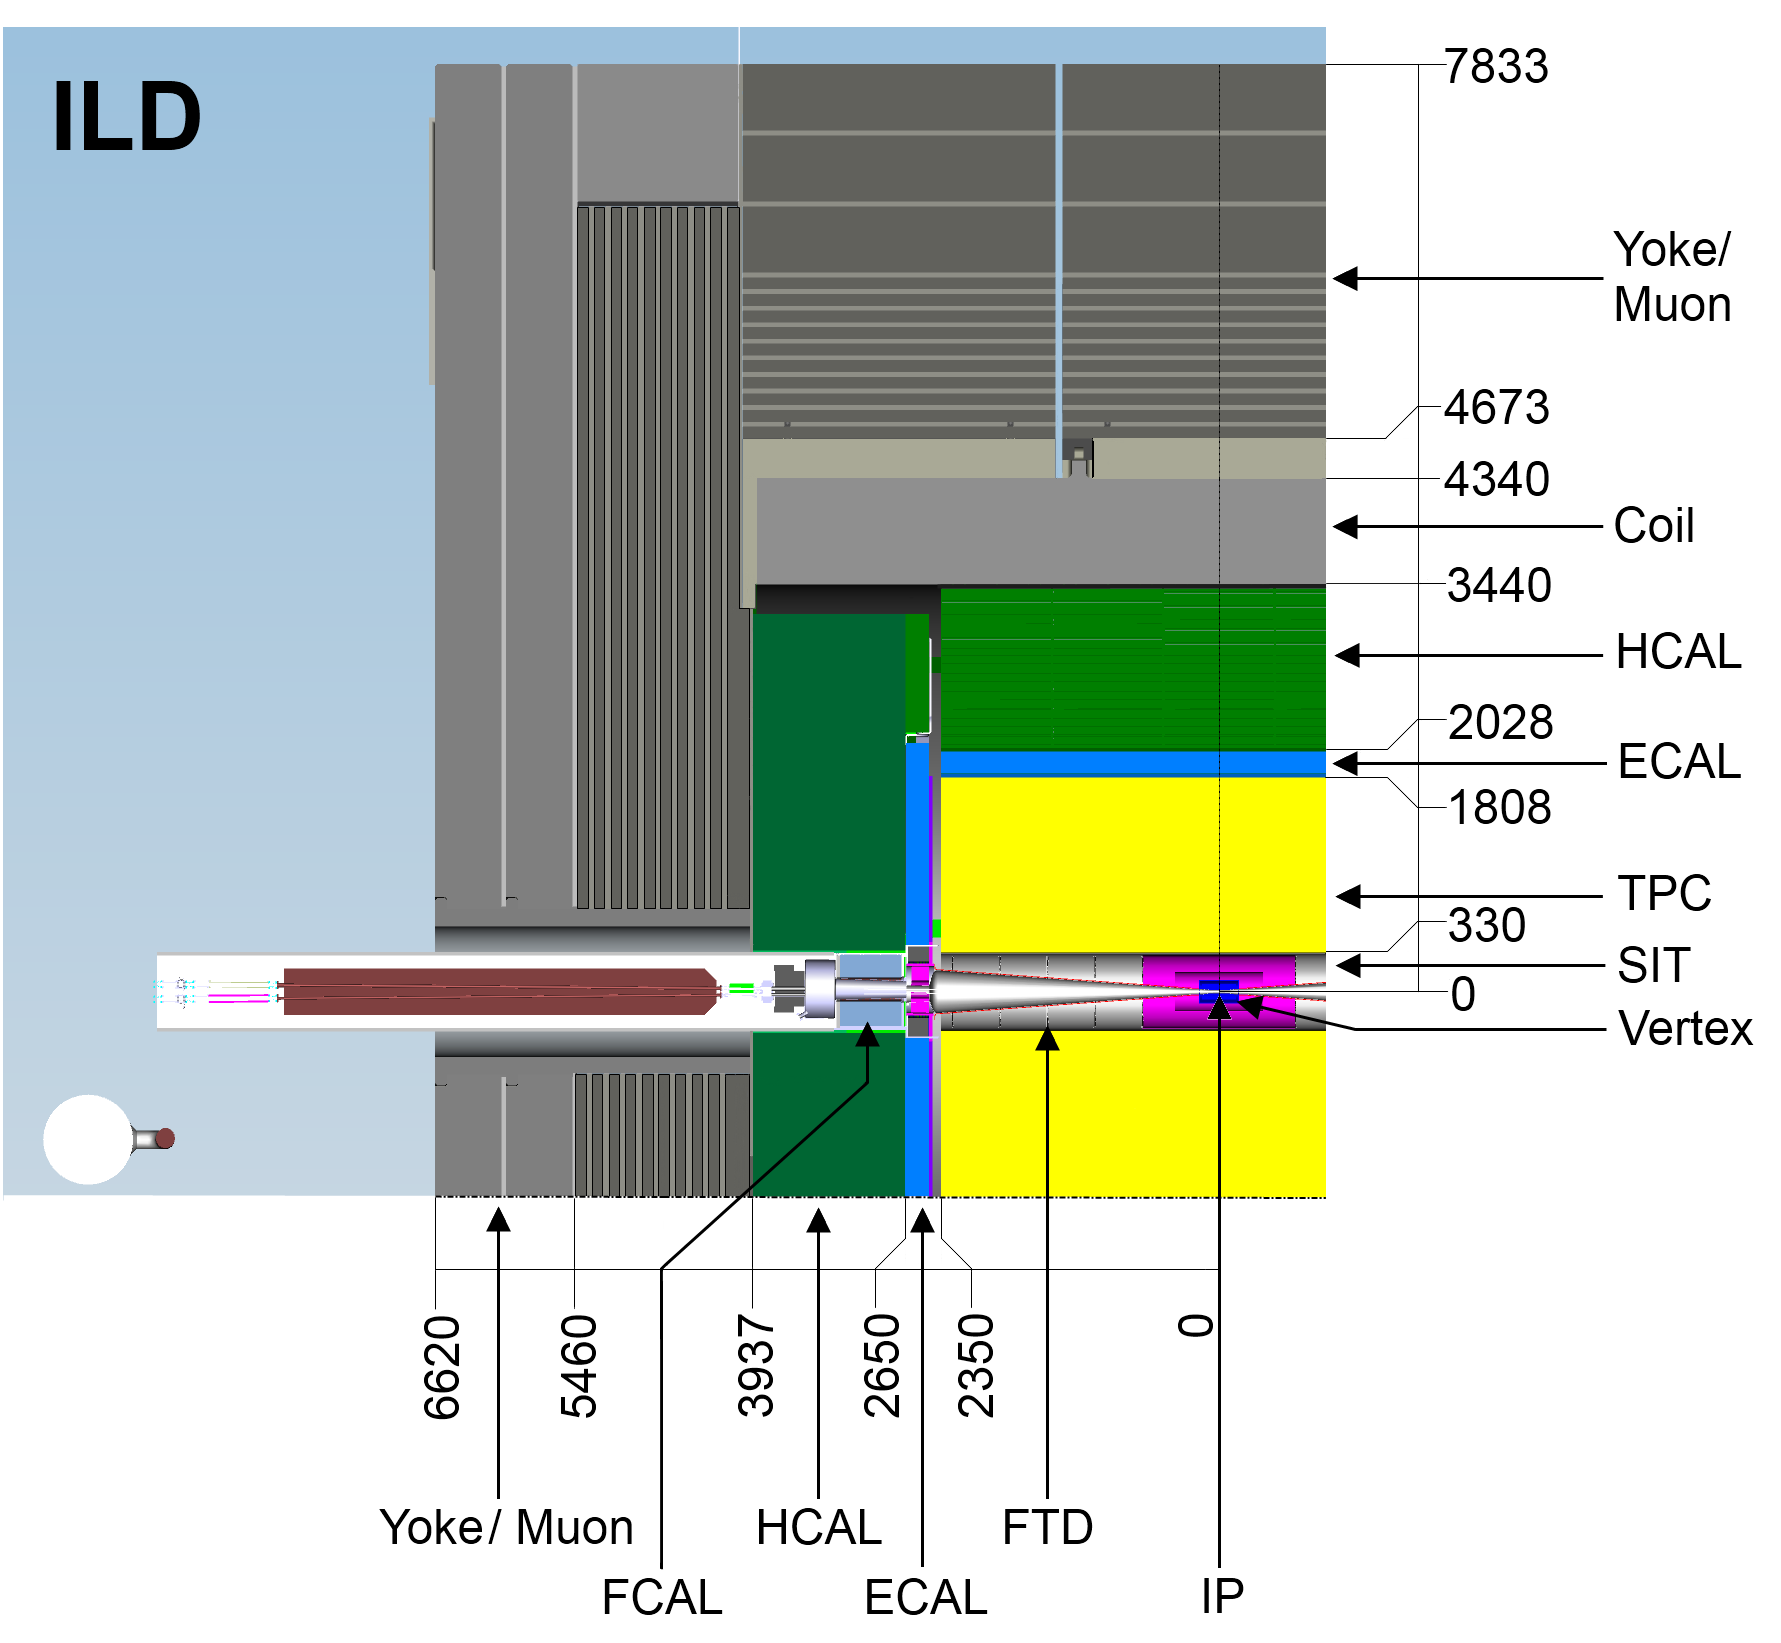
\includegraphics[width=0.8\hsize]{Detector/fig/ILD_quadrant_2.png}
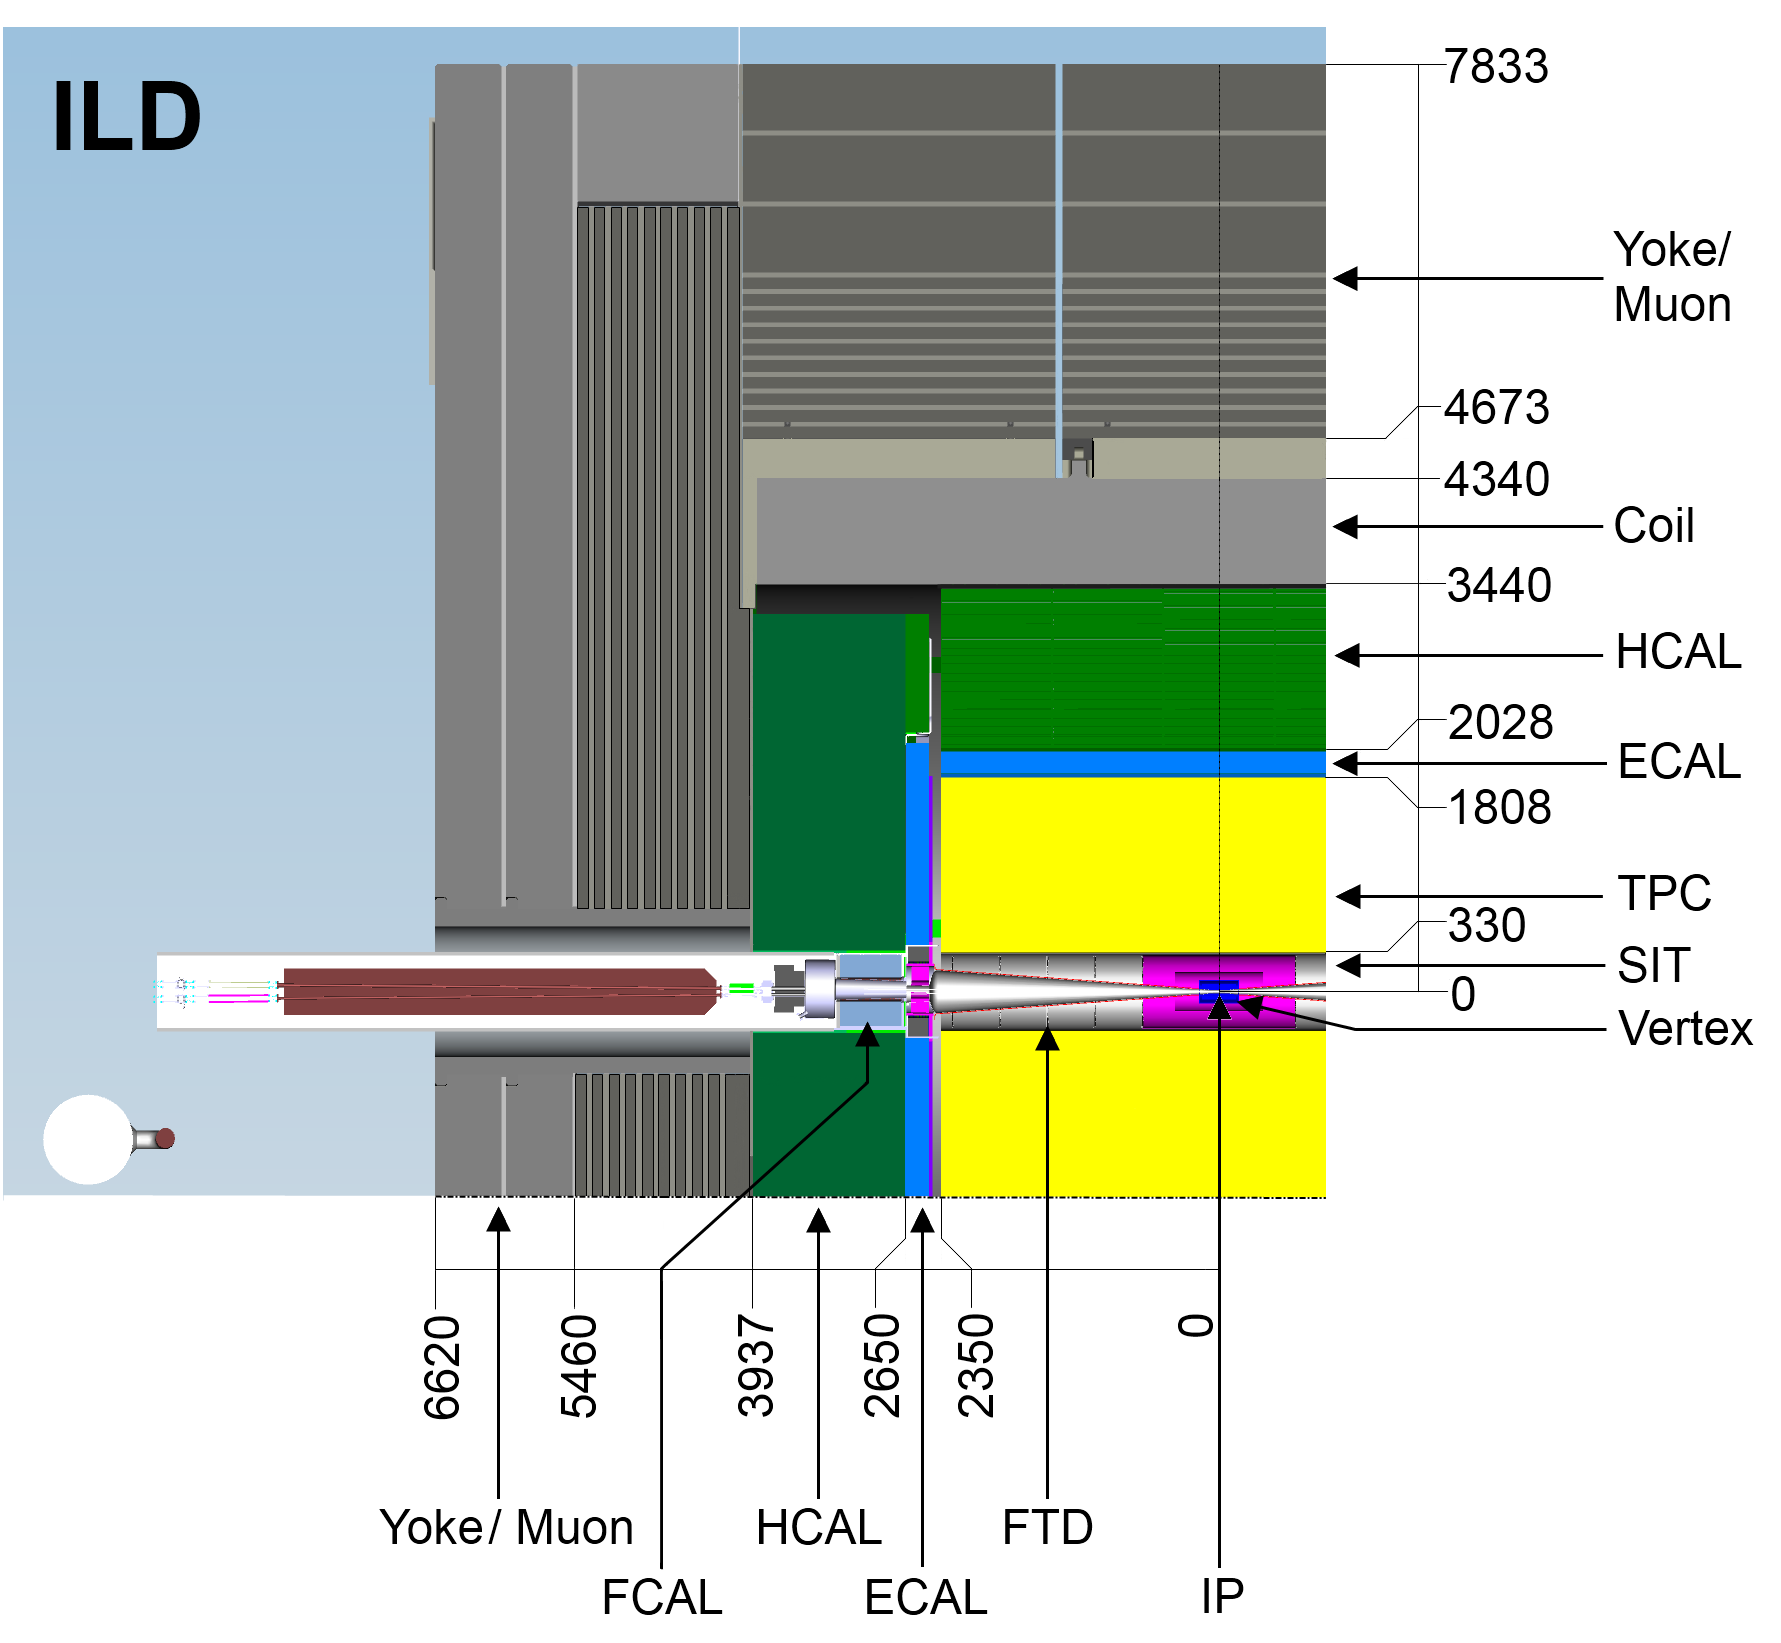
\includegraphics[width=0.6\hsize]{Detector/fig/ILD_quadrant_2.png}
\caption{r-z structure of an ILD quadrant.}
\label{fig:det:quad}
\end{figure}

The overall ILD detector structure is shown in figure ~\ref{fig:det:quad}: a high precision vertex detector positioned very close to the interaction point is followed by a hybrid tracking layout, realised as a combination of silicon tracking with a time projection chamber, and a calorimeter system. The complete system is located inside a large solenoid providing a nominal magnetic field of 3.5T (large ILD) or 4T(small ILD) . On the outside of the coil, the iron return yoke is instrumented as a muon system and as a tail catcher calorimeter. 
The main geometrical parameters are summarised in table~\ref{ild:tab:barrelpara} and table~\ref{ild:tab:endcappara}.
%\begin{sidewaystable}[thb]
\begin{table}\hspace*{-0cm}\small
%\begin{tabular}{|l|p{0.8cm}p{0.8cm}p{1.0cm}|p{2.5cm}p{3.0cm}p{3.0cm}|}
%\begin{tabular}{|l|p{0.06\textwidth}p{0.06\textwidth}p{0.07\textwidth}|p{0.25\textwidth}p{0.20\textwidth}p{0.20\textwidth}|}
\begin{tabular}{ l p{0.05\hsize}p{0.04\hsize}p{0.04\hsize} p{0.20\hsize}p{0.20\hsize}p{0.20\hsize} }
%\hline
\toprule
\multicolumn{7}{l}{{\bf Barrel system}}\\
%\hline
\midrule
System & R(in) & R(out) & z & \multicolumn{3}{l}{comments}\\
       & \multicolumn{3}{c}{[mm]}   &&&\\
%\hline
\midrule
VTX    & 16         & 60        & 125 & 3 double layers &  Silicon pixel sensors, & \\
       &            &           &           & layer 1: & layer 2: & layer 3-6 \\
       &            &           &           & $\sigma<3 \mu m$ & $\sigma < 6 \mu m$ & $\sigma < 4 \mu m$ \\
Silicon &           &           & &&&\\
- SIT   & 153       & 300       & 644   & 2 silicon strip layers & $\sigma = 7 \mu m$& \\
- SET   & 1811      &           & 2300   & 2 silicon strip layers & $\sigma = 7 \mu m$& \\
- TPC   & 330       & 1808      & 2350   & MPGD readout & $1 \times 6 $mm$^2$ pads & $\sigma=60 \mu m$ at zero drift \\
%\hline
\midrule
ECAL    & 1843      & 2028      & 2350   & W absorber  & SiECAL & 30 Silicon sensor layers, $5 \times 5$ mm$^2$ cells \\
        &           &           &        &             & ScECAL & 30 Scintillator layers,  $ 5\times 45$ mm$^2$ strips \\
HCAL    & 2058      & 3410      & 2350   & Fe absorber & AHCAL & 48 Scintillator layers, $3 \times 3$cm$^2$ cells, analogue \\
        &           &           &         &            & SDHCAL & 48 Gas RPC layers, $1\times 1$ cm$^2$ cells, semi-digital\\
%\hline
\midrule
Coil    & 3440      & 4400      & 3950    & 3.5 T field & $ 2 \lambda $& \\
Muon    & 4450      & 7755      & 2800    & 14 scintillator layers& &\\
%\hline
\bottomrule
\end{tabular}
\caption{\label{ild:tab:barrelpara}List of the main parameters of the ILD detector for the barrel part.}
\end{table}

\begin{table}\hspace*{-0cm}\small
%\begin{tabular}{|l|p{0.8cm}p{0.8cm}p{1.0cm}|p{2.5cm}p{3.0cm}p{3.0cm}|}
\begin{tabular}{ l p{0.05\hsize}p{0.04\hsize}p{0.04\hsize} p{0.20\hsize}p{0.20\hsize}p{0.20\hsize} }

%\hline
\toprule
\multicolumn{7}{ l }{{\bf End cap system}}\\
\midrule
System & z(min) & z(max) & r(min), r(max) & \multicolumn{3}{l}{comments}\\
       & \multicolumn{3}{c}{[mm]}   &&&\\
\midrule

FTD    & 220     & 371    &      & 2 pixel disks & $\sigma=2-6 \mu m$ &\\
       &         &        &      & 5 strip disks & $\sigma = 7 \mu m$& \\
ETD    & 2420    & 2445   & 419-1822 & 2 silicon strip layers & $\sigma=7 \mu m$ & \\
\midrule
ECAL   & 2450    & 2635   &      & W-absorber & SiECAL & Si readout layers \\
       &         &        &      &            & ScECAL & Scintillator layers \\
HCAL   & 2650    & 3937   & 335-3190& Fe absorber & AHCAL & 48 Scintillator layers $3 \times 3 $cm$^2$ cells, analogue\\
       &         &        &      &              & SDHCAL & 48 gas RPC layers $1\times 1$cm$^2$ cells, semi-digital \\
BeamCal & 3595   & 3715   & 20-150  & W absorber& 30 GaAs readout layers & \\
Lumical & 2500   & 2634   & 76-280 & W absorber & 30 Silicon layers & \\
LHCAL   & 2680   & 3205   & 93-331 & W absorber &&\\
\midrule
Muon    & 2560   &        & 300-7755 & 12 scintillator layers&&\\
\bottomrule
\end{tabular}
\caption{\label{ild:tab:endcappara}List of the main parameters of the ILD detector for the end cap part.}

\end{table}

A key characteristics of the detector is the amount of material crossed by the particles: particle flow requires a thin tracker to minimise interactions before the calorimeters, and thick calorimeters to fully absorb the showers and measure neutral hadrons. Figure~\ref{fig:det:material} shows the amount of radiation lengths of the trackers material and the total interaction lengths including the calorimeter system. 

\thisfloatsetup{floatwidth=\SfigwFull,capposition=beside}
\begin{figure}[t!]
\begin{tabular}{cc}
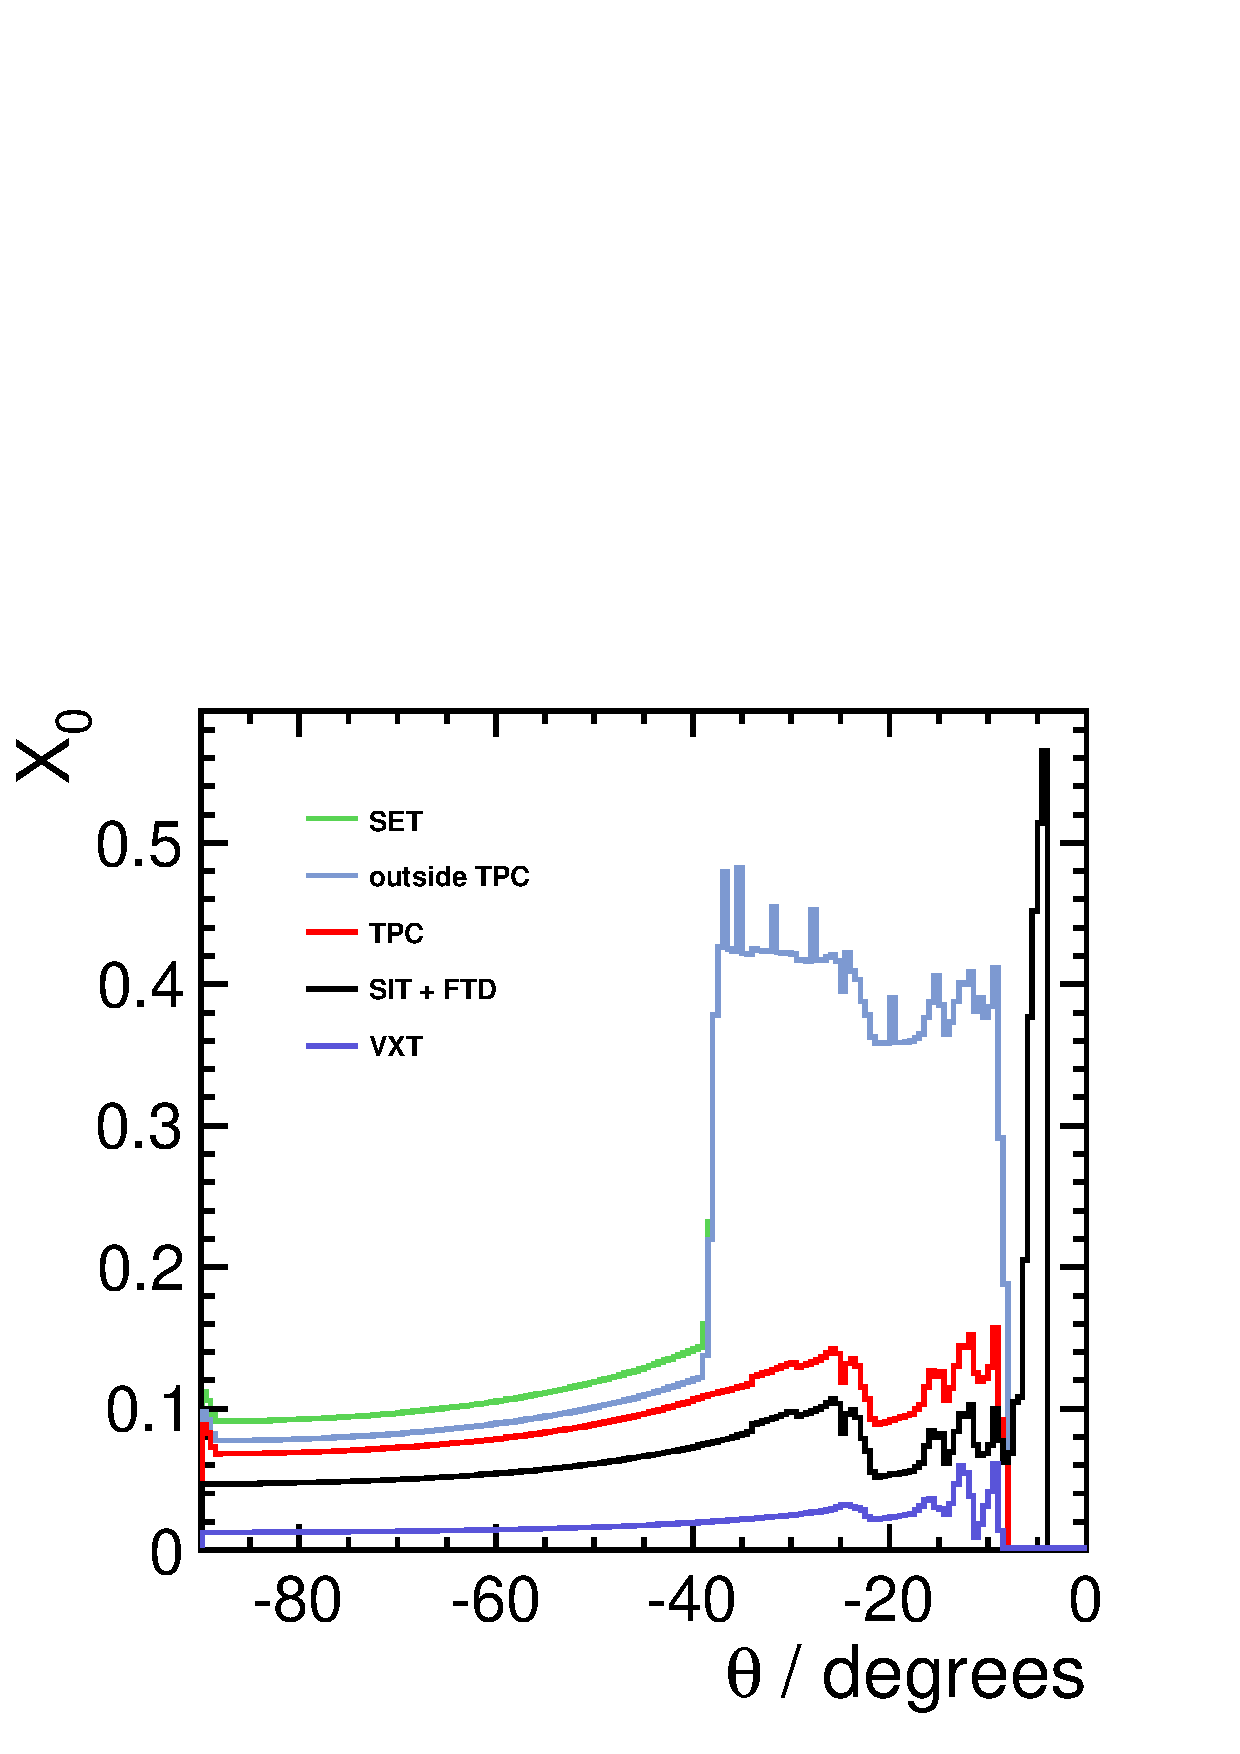
\includegraphics[width=0.52\hsize,viewport={0 -10 600 500},clip]{Detector/fig/material-budget-new.pdf} &
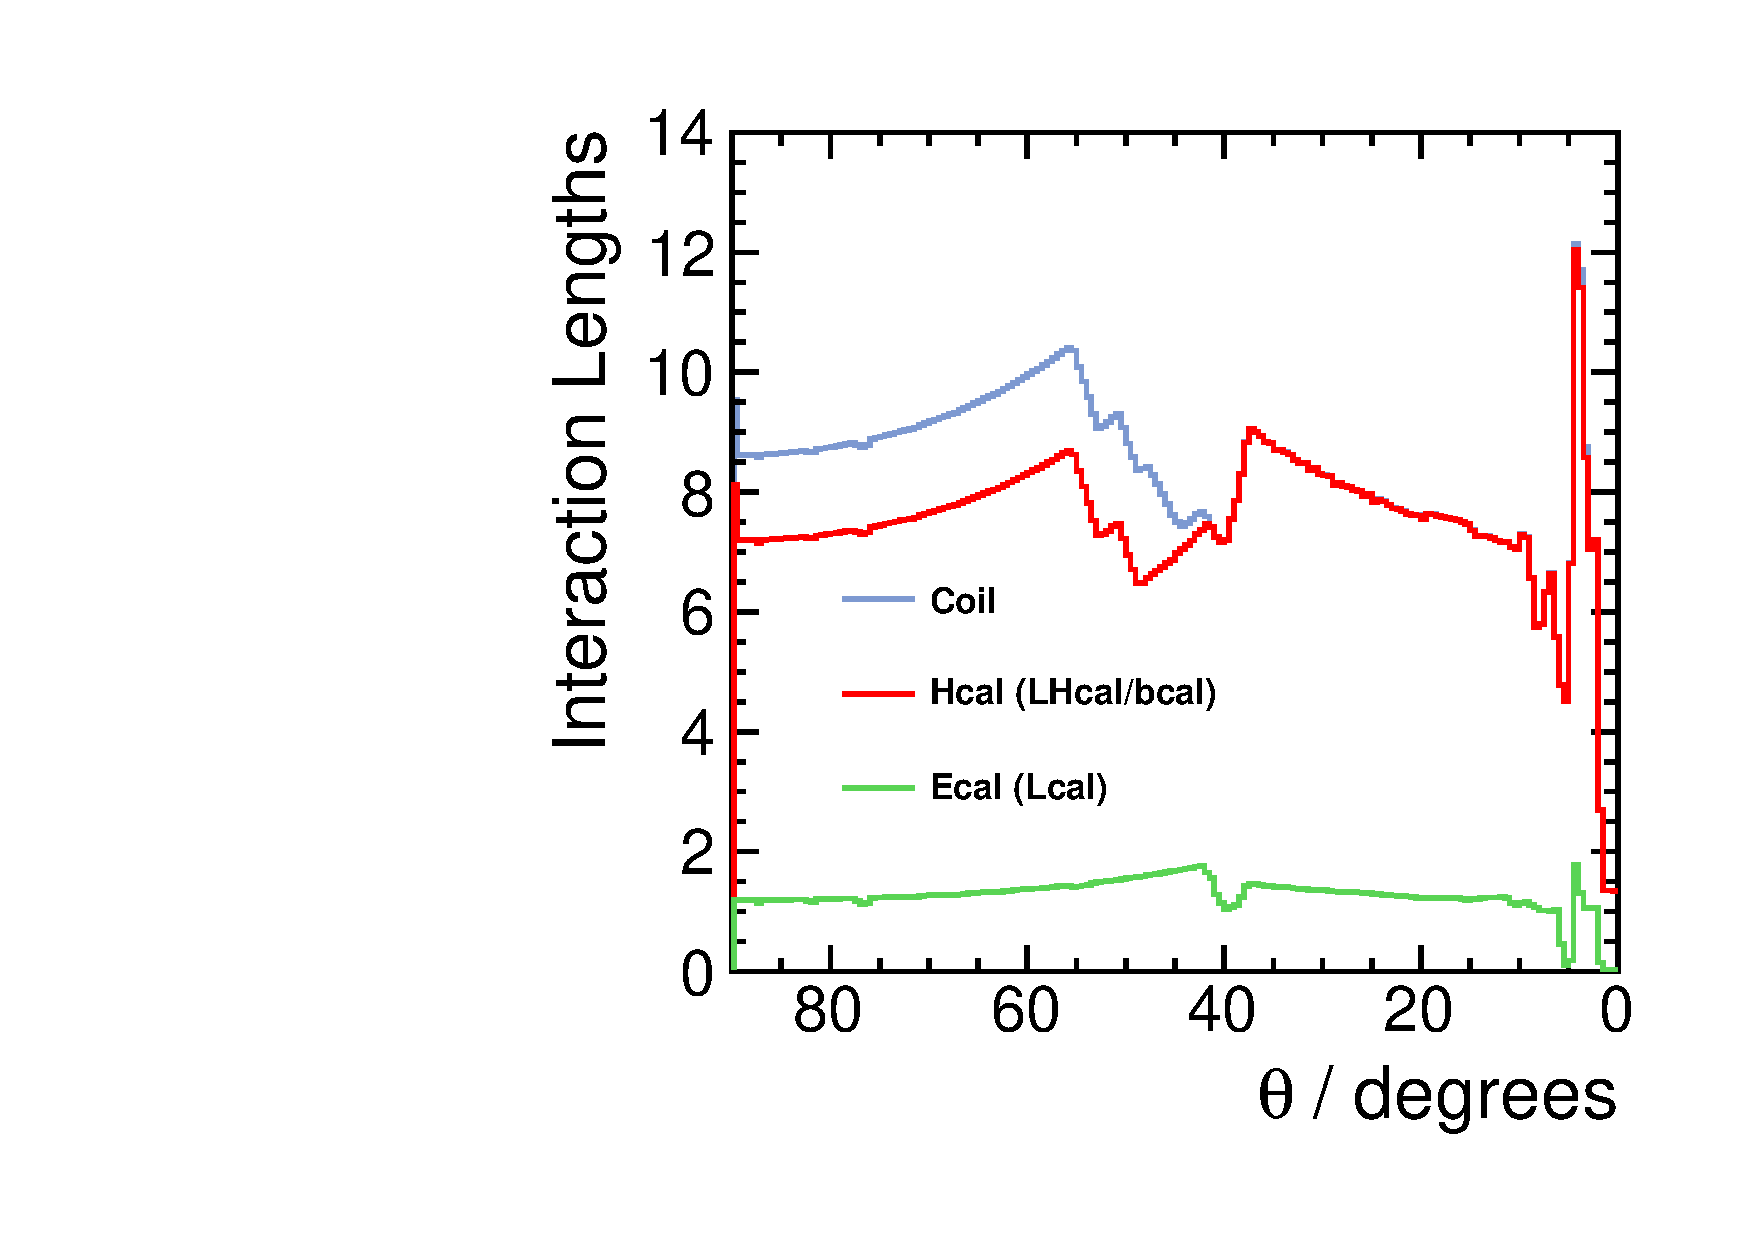
\includegraphics[width=0.5\hsize]{Detector/fig/intlen_ILD_o1_v05.pdf}
\end{tabular}
\caption[Material in the ILD detector]{Left: Average total radiation length of the trackers material as a function of polar angle. Right: Total interaction length seen up to the end of the electromagnetic calorimeter, the hadronic calorimeter and the solenoid coil, respectively.}
%\end{figure}
\label{fig:det:material}
%\begin{tabular}{cc}

\end{figure}

\vspace{2cm}
\subsection{Subdetector layouts}
\writer{Subdetector technical conveners}{4}

The current design of subdetectors is presented including open options and critical aspects, as well as prospects for enhanced capabilities in the future. The most recent progress and status of each detection technology will be summarized in section 5.2.

\vspace{1cm}
\subparagraph*{\bf Vertex detector}
\textit{(Besson, Ishikawa, Vos)}

The vertex detector (VTX, Figure~\ref{fig:det:vertex}) is realised as a multi-layer pixel detector with three double-layers. The detector has a pure barrel geometry. To minimise the occupancy from background hits,
the first double-layer is only half as long as the outer two. 



\begin{figure}[t!]
\centering
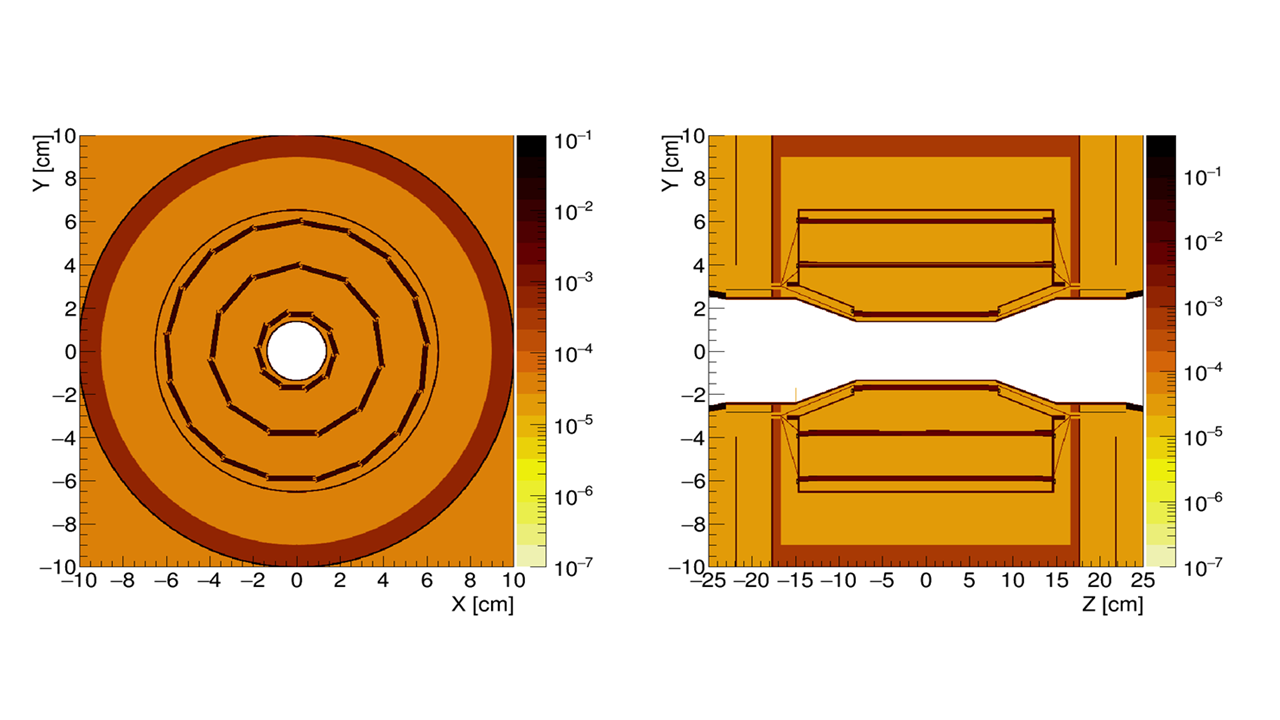
\includegraphics[width=0.6\hsize]{Detector/fig/vertex.png}
\caption{layout of the vertex detector.}
\label{fig:det:vertex}
\end{figure}

Critical parameters of the VTX optimisation are the point resolution for secondary vertex tagging and the material thickness for minimal multiple scattering. Three main technologies are under consideration to achieve the required goals:
\begin{itemize}
    \item {\bf CMOS pixels:} this well-established technology offers the advantages of high granularity with fully monolythic pixel digital electronics available from industrial processes. The most critical points of focus of current R\&D are the readout speed for bunch crossing tagging, the power consumption and the overall material budget of the layers.
    \item {\bf DEPFET pixels:} this technology offers the advantage of high granularity with a small layer material thickness, the digital electronics being shifted at the end of the ladders. Critical aspects are the industrialisation of the fabrication process and the integration of large detector surfaces.
    \item{\bf Fine Pixel CCD (FPCCD):} CCD's offer the prospects for the highest granularities associated with low power consumption. Another advantage is the minimal material budget of the detector layer, however counter-balanced by the need of a cryostat to ensure low-temperature operation. Critical aspects under study are the readout speed and the resistance to radiation.  
\end{itemize}

\vspace{0.5cm}
The CMOS and DEPFET pixels have typical sizes of 20 microns and are readout in a continuous mode during bunch trains. The readout speed determines the capability to resolve individual bunches. The FPCCD pixels accumulate hits during one bunch train before readout and reset in-between trains. Their occupancy is kept acceptable thanks to a small pixel size of order 5 microns.  


\vspace{1cm}
\subparagraph*{\bf Silicon trackers}
\textit{(Besson, Vos, Vila)}

A system of silicon trackers surrounds the VTX detector. In the barrel, two layers of silicon detectors (SIT) are arranged to bridge the gap between the VTX and the TPC, and one silicon outer layer (SET) is foreseen inbetween the TPC and the ECAL. In the forward region, a system of seven silicon disks (FTD) provides low angle tracking coverage (Figure~\ref{fig:det:FTD}).

\begin{figure}[t!]
\centering
%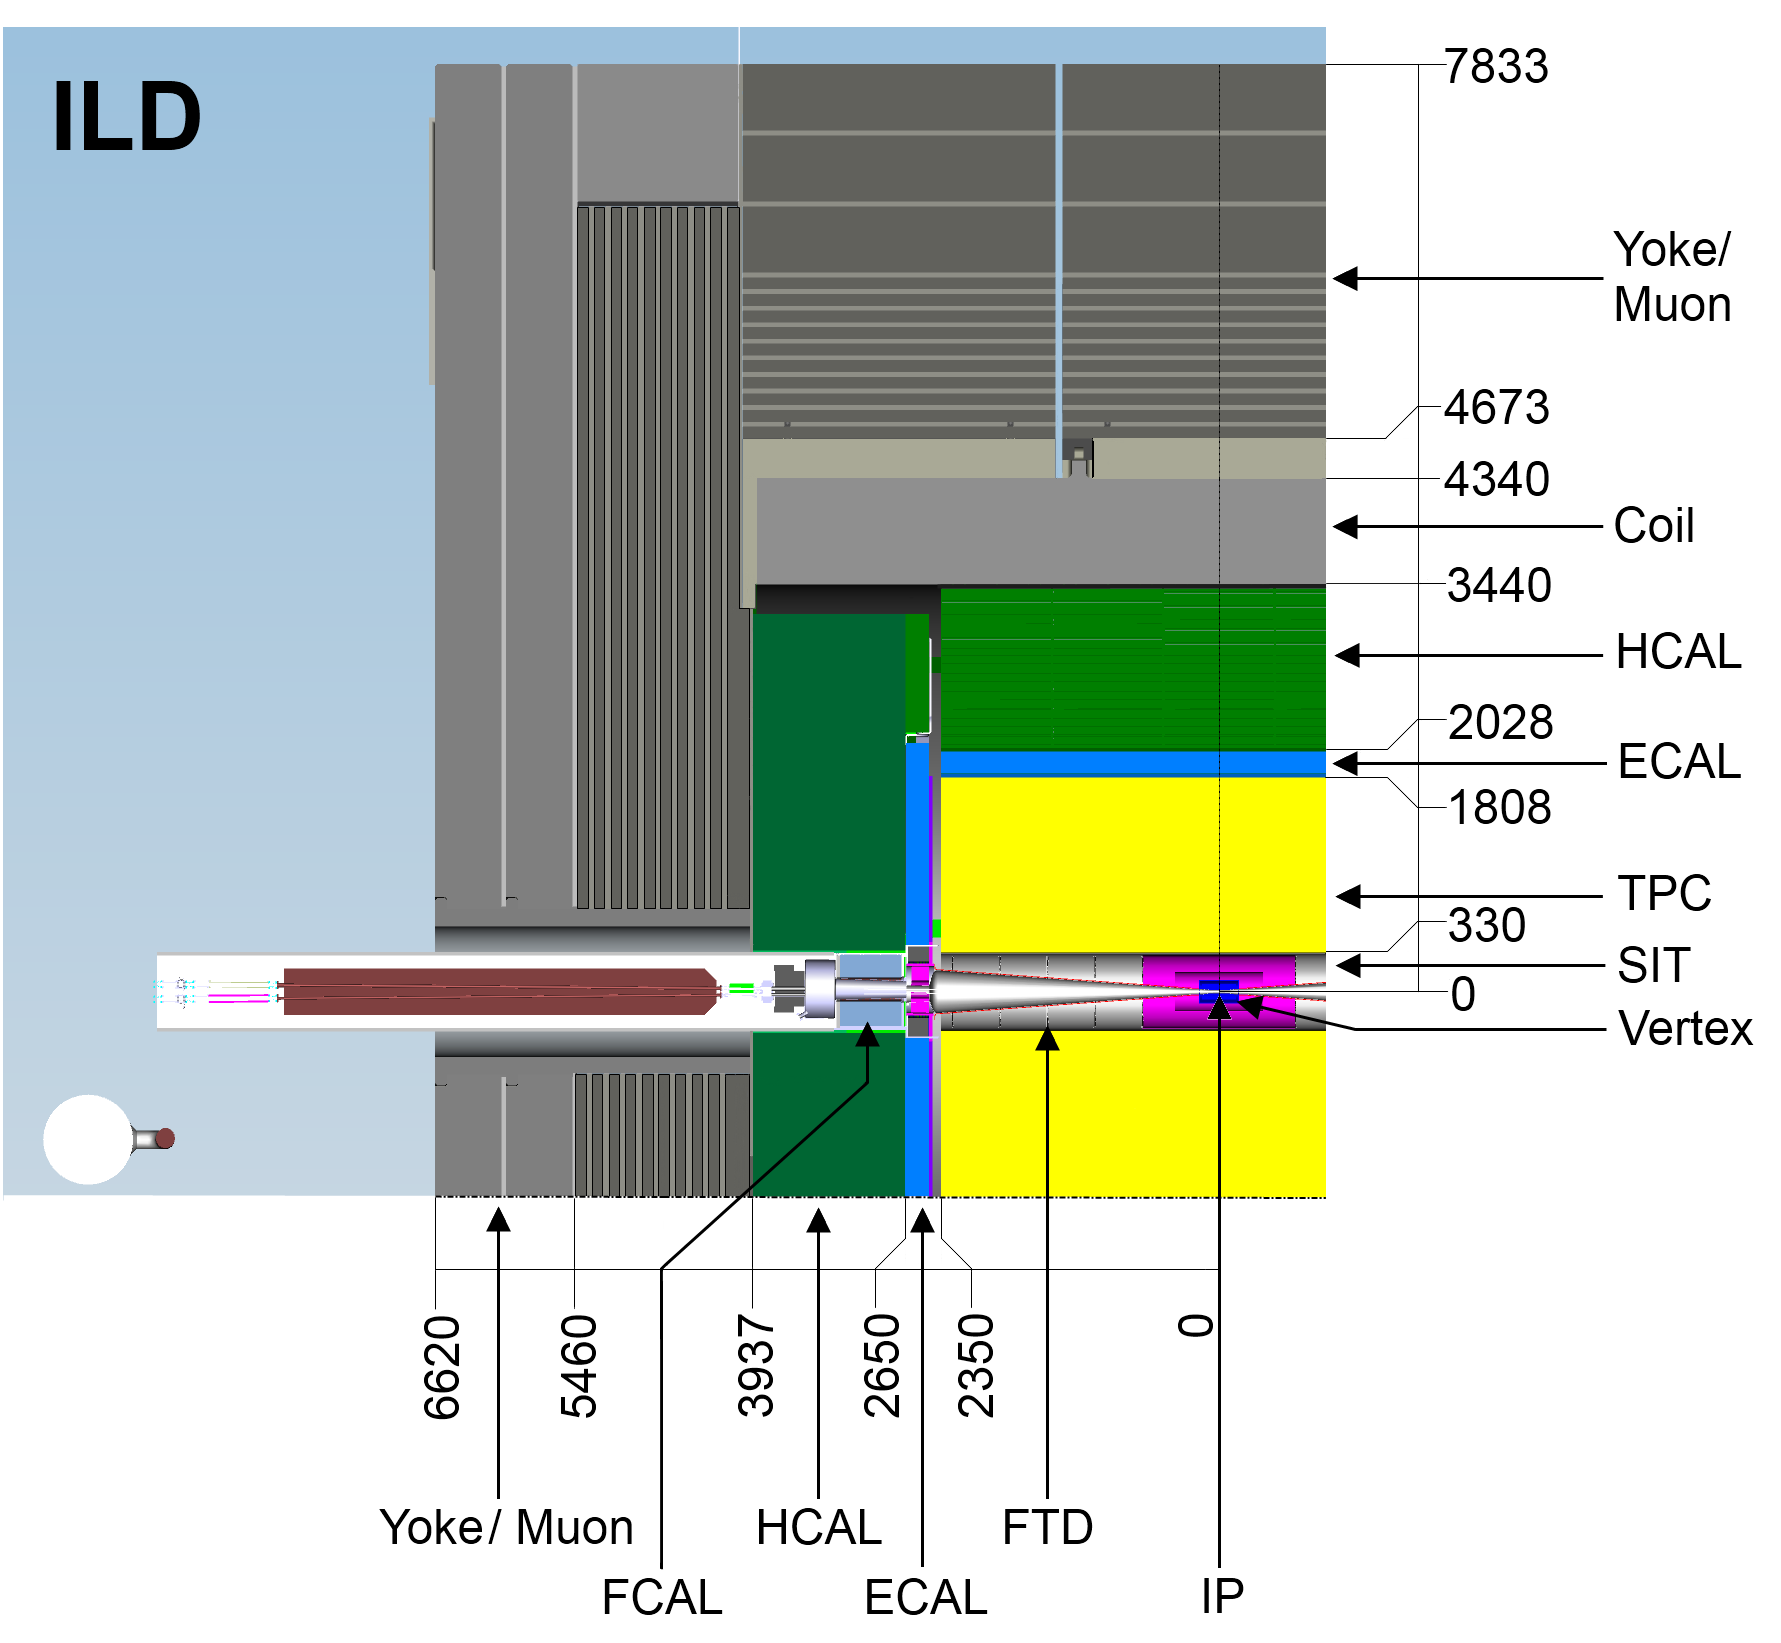
\includegraphics[width=0.8\hsize]{Detector/fig/ILD_quadrant_2.png}
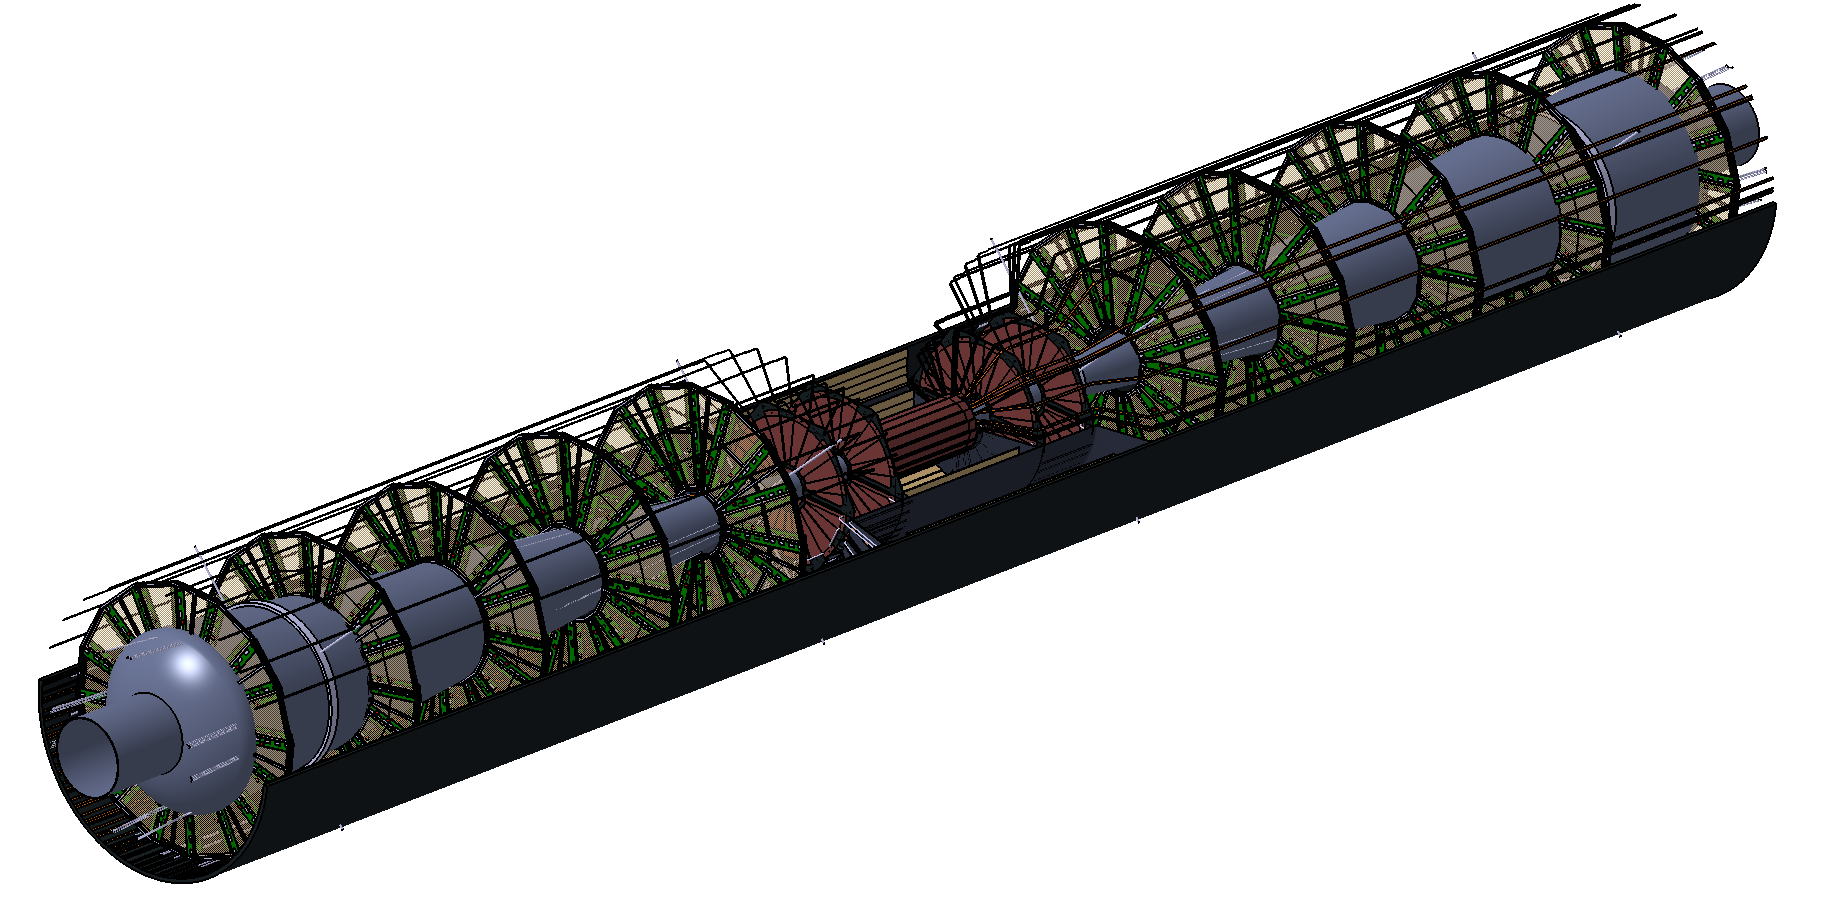
\includegraphics[width=0.75\hsize]{Detector/fig/FTD.png}
\caption{layout of the Forward Tracking Detector.}
\label{fig:det:FTD}
\end{figure}

The baseline technology for the large area trackers is silicon strips but it is considered to move to pixel wherever possible: pixels are already the baseline for the two inner FTD disks, for which the current choice is DEPFET pixels. The possibility to equip more FTD disks with pixels is under study to improve track reconstruction efficiency in the forward region. The progress made with CMOS detectors may also allow to equip the SIT with pixels instead of strips. The design of the SET is still open including the option to implement it as the first layer of the ECAL Calorimeter. The use of high resolution timing detectors is considered in order to provide a TOF functionality for particle identification.   

\vspace{1cm}
\subparagraph*{\bf TPC}
\textit{(Colas, Sugiyama)}

A distinct feature of ILD is a large volume time projection chamber (Figure~\ref{fig:det:TPC} left). The TPC advantages are 3-dimensional point resolution, d$E$/d$x$ based particle identification and minimum material in the field cage. One critical issue concerns potential field distorsions due to ion accumulation within the chamber. At ILC this can be mitigated by implementating an ion gating between bunch trains: ions produced in the gas amplication region during bunch trains are confined and eliminated outside bunch trains by reverting the electric field configuration. This can be implemented with GEM foils as shown in Figure~\ref{fig:det:TPC} right.

%\thisfloatsetup{floatwidth=\SfigwFull,capposition=beside}
\begin{figure}[t!]
\begin{tabular}{cc}
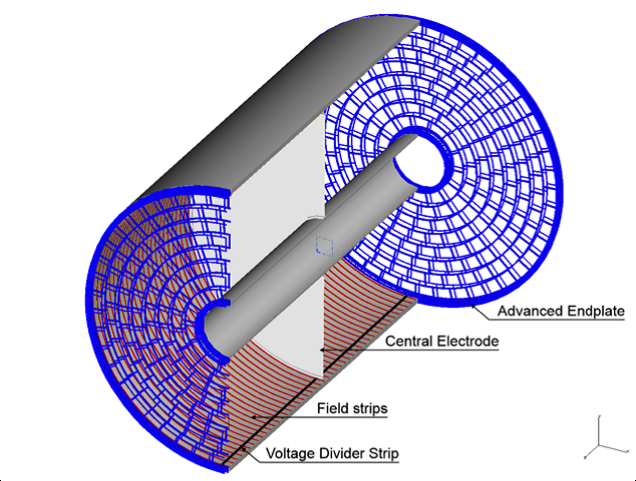
\includegraphics[width=0.6\hsize,viewport={0 -10 600 500},clip]{Detector/fig/TPC.png} &
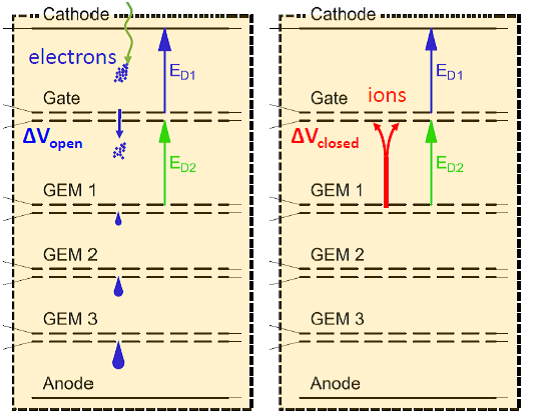
\includegraphics[width=0.4\hsize]{Detector/fig/gating.png}
\end{tabular}
\caption[TPC layout]{Left: Glogal layout of the TPC chamber. Right: Principle of the ion GEM gating scheme showing the two electric field configurations within (left) and outside (right) bunch trains.}
%\end{figure}
\label{fig:det:TPC}
%\begin{tabular}{cc}
\end{figure}

Three options are under consideration for the ionisation signal amplification and readout:
\begin{itemize}
    \item GEM readout (Figure~\ref{fig:det:TPC_readout} left): the ionisation signal is amplified by passing through a GEM foil and is collected on pads.
    \item Micromegas readout (Figure~\ref{fig:det:TPC_readout} right): the ionisation signal is amplified between a mesh and the pad array where it is collected.
    \item GRIDPIX: the ionisation signal is amplified as for the micromegas case but collected on a fine silicon pixel grid providing individual pixel timing.
\end{itemize}
\vspace{0.5cm}
For the GEM and micromegas options, the typical pad sizes are a few mm (table~\ref{ild:tab:barrelpara}) and spatial resolution is improved by combining the track signals of several adjacent pads. For the GRIDPIX option the pixel size of $\approx$50 microns matches the size of the mesh, providing pixel sensitivity to single ionisation electrons. The spatial resolution is improved and the dE/dx signal measured by counting pixels. 

%\thisfloatsetup{floatwidth=\SfigwFull,capposition=beside}
\begin{figure}[t!]
\begin{tabular}{cc}
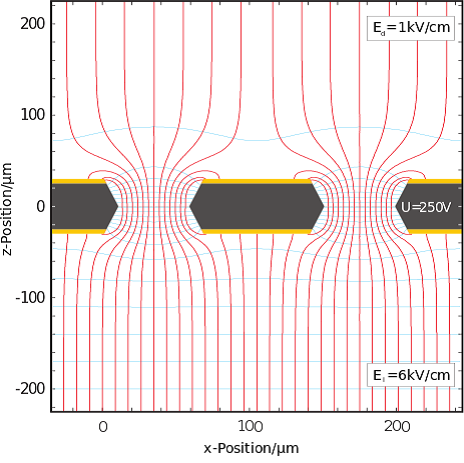
\includegraphics[width=0.5\hsize,viewport={0 -10 600 500},clip]{Detector/fig/GEM.png} &
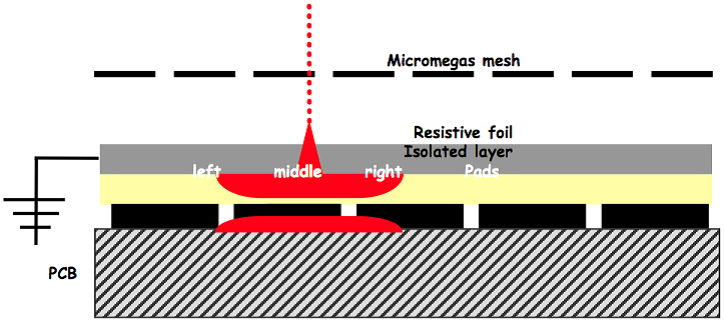
\includegraphics[width=0.4\hsize]{Detector/fig/micromegas.png}
\end{tabular}
\caption[TPC readout]{Amplication scheme of the TPC ionisation signals with GEM (left) and micromegas (right) readout.}
%\end{figure}
\label{fig:det:TPC_readout}
%\begin{tabular}{cc}
\end{figure}

\vspace{1cm}
\subparagraph*{\bf ECAL}
\textit{(Brient, Ootani)}

Electromagnetic showers are measured with a compact highly-segmented calorimeter (Figure~\ref{fig:det:ECAL}) whose absorber planes are made of tungsten. The ECAL barrel shape is octogonal with individual stacks laid such as to avoid projective dead zones in azimuth. The baseline number of layers is 30, with an option to reduce the number to 22 keeping the amount of radiation lengths identical and increasing the thickness of the sensitive medium to maintain a similar energy resolution.

\begin{figure}[t!]
\centering
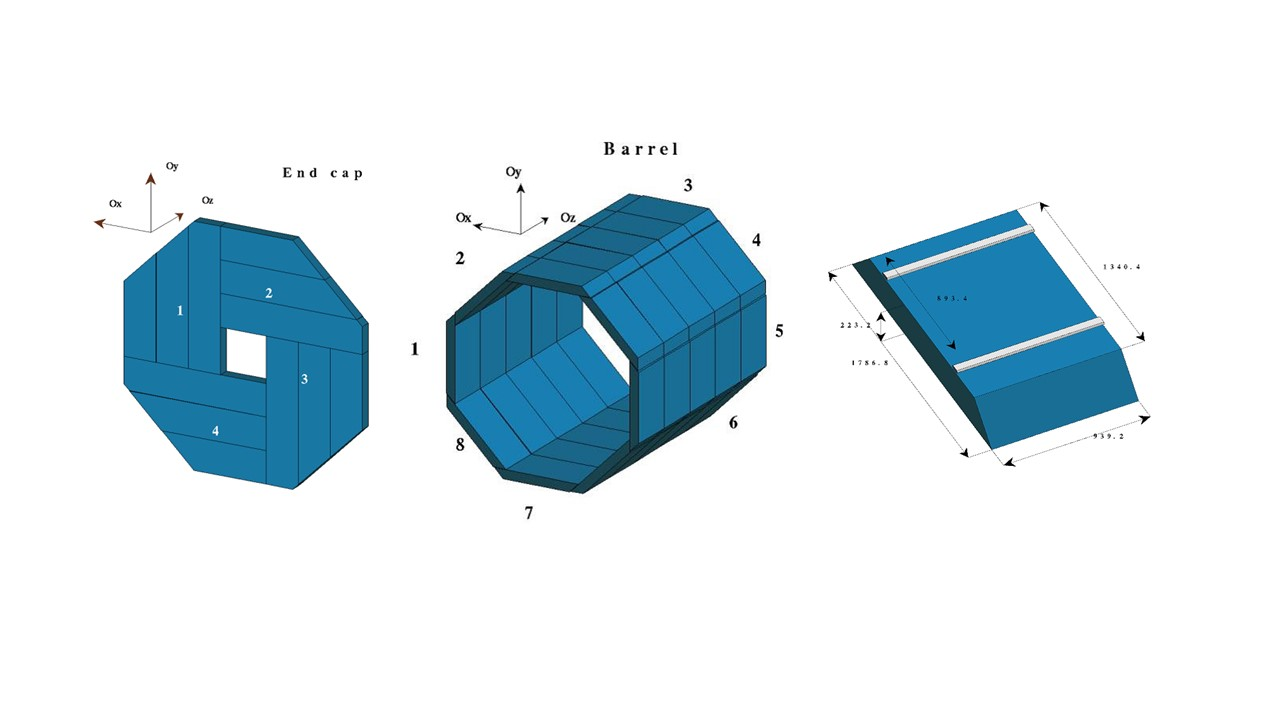
\includegraphics[width=1.2\hsize]{Detector/fig/ECAL_structure.jpg}
\caption{Mechanical structure of the electromagnetic calorimeter: left: endcap wall; center: barrel; right: individual barrel stack.}
\label{fig:det:ECAL}
\end{figure}

The sensitive medium consists in silicon sensors with 5x5 $mm^2$ pads bonded on a PCB equipped with front-end readout ASICs (Figure~\ref{fig:det:ECAL_readout} left). In order to reduce the costs it is also considered to equip part of the sensitive layers with scintillator sensors readout through SiPMs (Figure~\ref{fig:det:ECAL_readout} left). In that case the scintillator strips would have a larger dimension of 45x5$mm^2$ with alternate orthogonal orientation.  

\begin{figure}[t!]
\centering
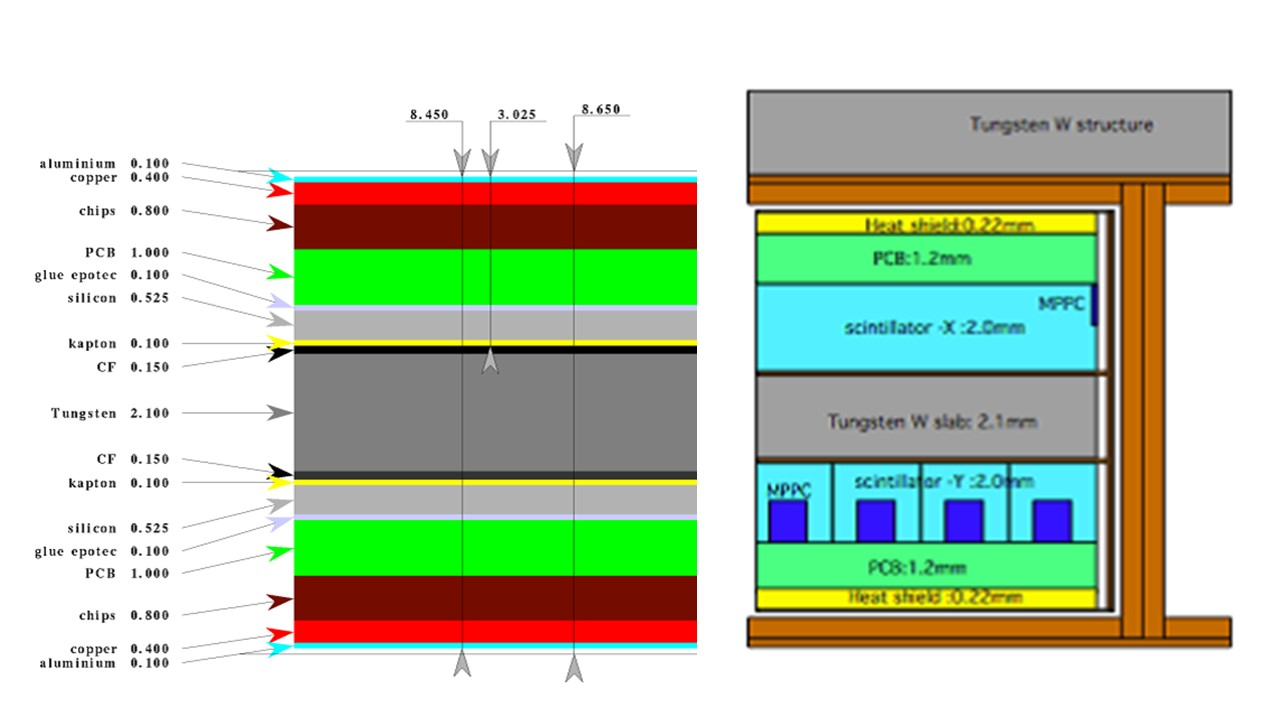
\includegraphics[width=1.0\hsize]{Detector/fig/ECAL_readout.jpg}
\caption{ECAL sensitive layer: left: silicium option; right: scintillator option.}
\label{fig:det:ECAL_readout}
\end{figure}


\vspace{1cm}
\subparagraph*{\bf HCAL}
\textit{(Laktineh, Sefkow)}

The hadronic calorimeter consists in 48 longitudinal samples with steel absorber plates. Two options are currently considered for the mechanical structure, differing mainly in the barrel region (Figure~\ref{fig:det:HCAL}): the "TESLA" barrel made of 2 wheels with signals extracted longitudinally in the gaps between the barrel and endcaps, and the "VIDEAU" barrel made of 3 to 5 wheels with signals extracted at the periphery between the HCAL and coil cryostat. The latter presents no dead zone in azimuth nor at $90^o$ polar angle, and offers a better mechanical stiffness, at the cost of a reduced accessibility of the front-end electronics.

\begin{figure}[t!]
\centering
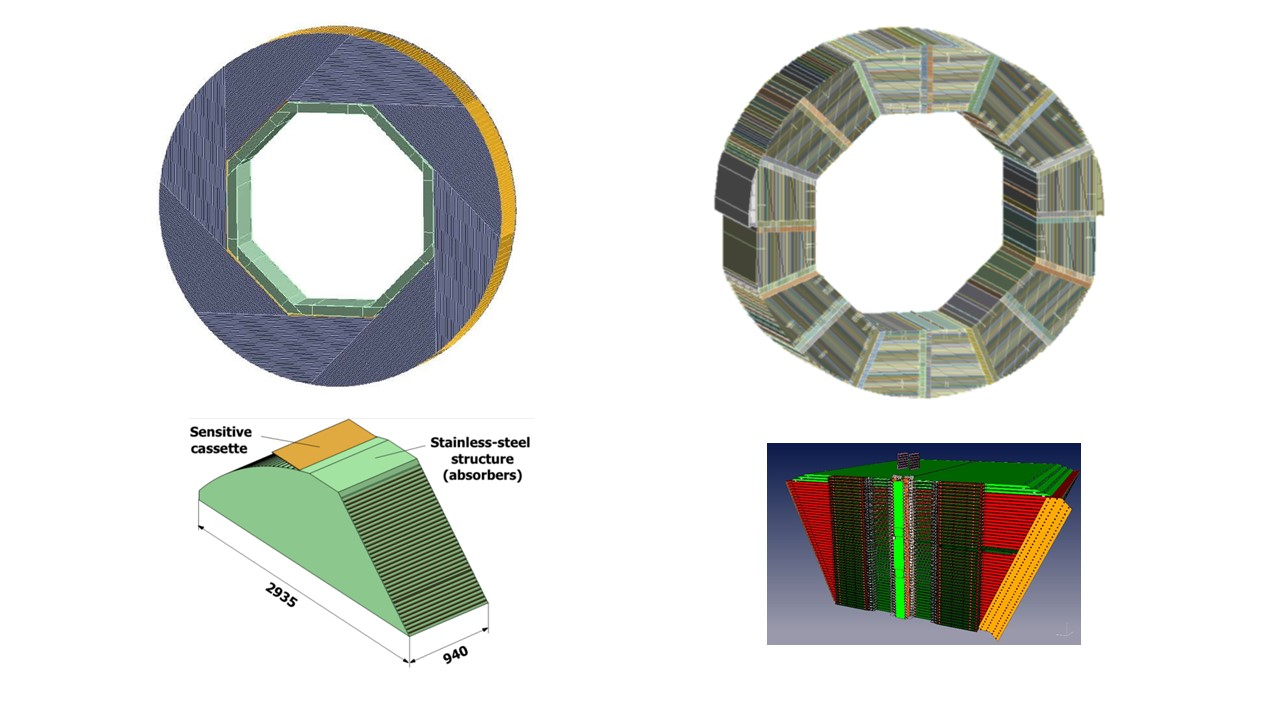
\includegraphics[width=1.1\hsize]{Detector/fig/HCAL_structure.jpg}
\caption{HCAL barrel mechanical structure: full wheel (top) and indiviual stack (bottom) for the two configurations under consideration: the "Videau" option (left) and the "TESLA" option (right).}
\label{fig:det:HCAL}
\end{figure}

The HCAL layers are instrumented with high granularity for an efficient separation of charged and neutral hadronic showers, necessary for particle flow, as well as for a good muon identification for flavor jet tagging. Two sensor options are under consideration (Figure~\ref{fig:det:HCAL_readout}): scintillator tiles of 3x3 $cm^2$ with analog readout through SiPMs, and RPC's with pads of 1 $cm^2$ readout with a semi-digital resolution of 2 bits.

\begin{figure}[t!]
\begin{tabular}{cc}
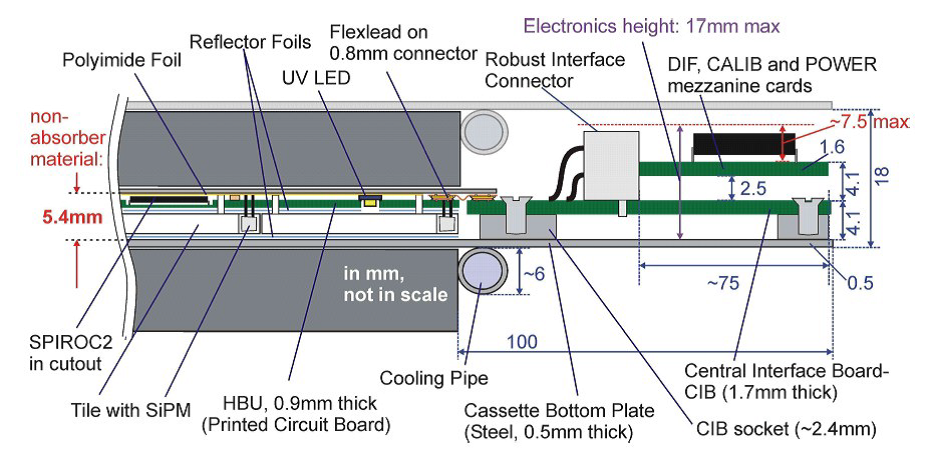
\includegraphics[width=0.5\hsize,viewport={0 -10 600 500},clip]{Detector/fig/AHCAL_layer.png} &
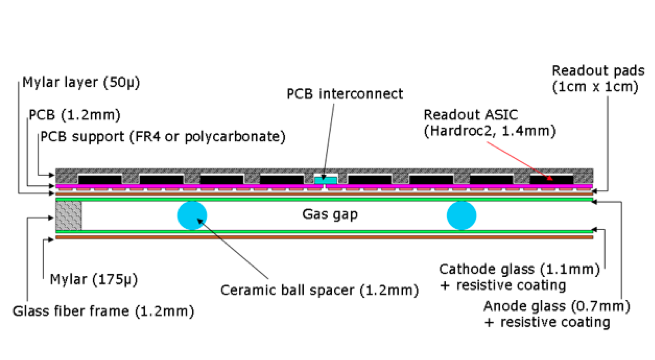
\includegraphics[width=0.5\hsize]{Detector/fig/SDHCAL_layer.png}
\end{tabular}
\caption{HCAL sensitive layer; left: scintillator option; right: RPC option.}
%\end{figure}
\label{fig:det:HCAL_readout}
%\begin{tabular}{cc}
\end{figure}


\vspace{1cm}
\subparagraph*{\bf VFS}
\textit{(Benhammou, Schuwalow)}

The ILD very forward region is equipped with dedicated detectors to perform:
\begin{itemize}
\item a precise determination of the luminosity from Bhabha scattering electron pairs (LumiCAL);
\item an extension of the hadronic calorimetry coverage in the forward region (LHCAL);
\item calorimetric hermeticity down to the beam pipe and fast monitoring of beam conditions (BeamCAL).
\end{itemize}
The overall layout of the detectors is shown in Figure~\ref{fig:det:VFS} left. Their longitudinal positioning has been adapted as shown in Figure~\ref{fig:det:VFS} right to account for the new ILC optics (chapter 3).  

\begin{figure}[t!]
\centering
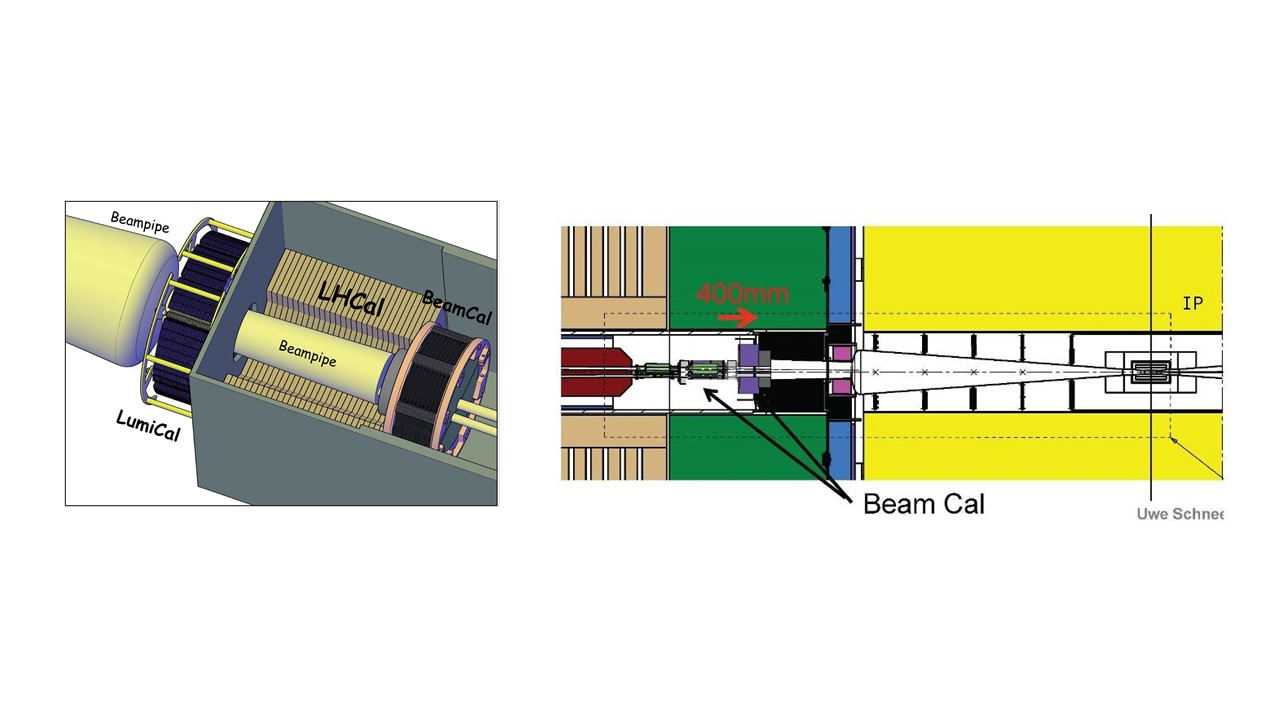
\includegraphics[width=1.0\hsize]{Detector/fig/VFS.jpg}
\caption{Overal layout of the Very Forward detectors (left) and adaptations performed for the new ILC optics (right).}
\label{fig:det:VFS}
\end{figure}

The very forward detectors are based on similar technologies as the ILD electromagnetic calorimeter, taking into account the specific conditions of the forward region such as the harder radiation environment or the need for an improved compactness to identify electromagnetic showers in a high occupancy environment. For the detectors positioned closest to the beam pipe new sensors such as saphire are considered. The LumiCAL has the most advanced design and will be based on silicon sensors similar to the ECAL (Figure~\ref{fig:det:lumical}), with thinner instrumentation layers to minimize the lateral spread of the showers .     

\begin{figure}[t!]
\centering
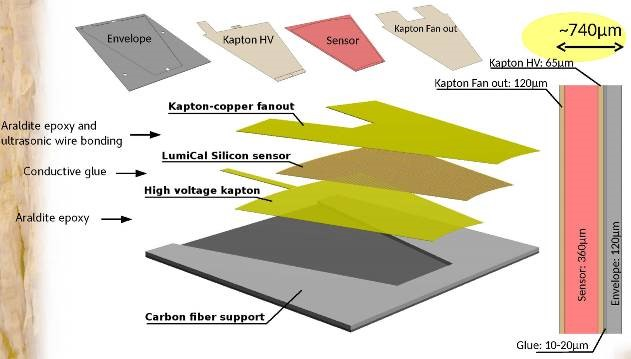
\includegraphics[width=0.8\hsize]{Detector/fig/lumical_layer.jpg}
\caption{Structure of a sensitive layer of the LumiCAL calorimeter.}
\label{fig:det:lumical}
\end{figure}

\vspace{1cm}
\subparagraph*{\bf Iron instrumentation}
\textit{(Saveliev)}

A large volume superconducting coil surrounds the calorimeters, creating an axial $B$-field of nominally 3.5 Tesla (large ILD) or 4 Tesla (small ILD). An iron yoke returns the magnetic flux of the solenoid, and, at the same time, serves as a muon filter, muon detector and tail catcher calorimeter. The baseline structure of the yoke is shown in Figure~\ref{fig:det:yoke} left for a configuration accounting for the maximum stray fields allowed in the push-pull configuration (chapter 3). Optimisation of the yoke size is ongoing to minimize the overal cost driven by the amount of iron. A number of iron yoke gaps will be instrumented for muon tracking and measurement of the tails of the hadronic showers. The instrumentation is expected to consist in scintillator bars read with SiPMs (Figure~\ref{fig:det:yoke} right) but RPCs are also considered.   

\begin{figure}[t!]
\begin{tabular}{cc}
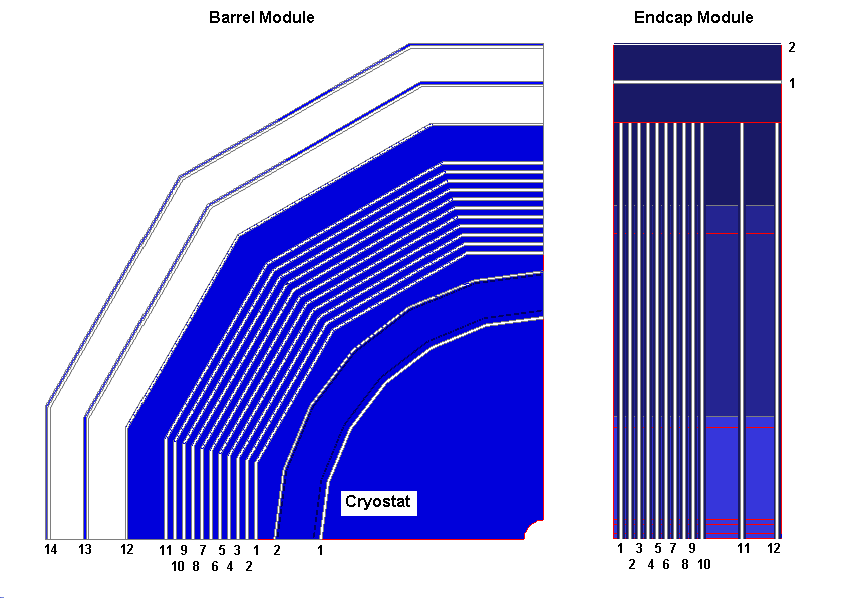
\includegraphics[width=0.5\hsize,viewport={0 -10 600 500},clip]{Detector/fig/yoke_layout.png} &
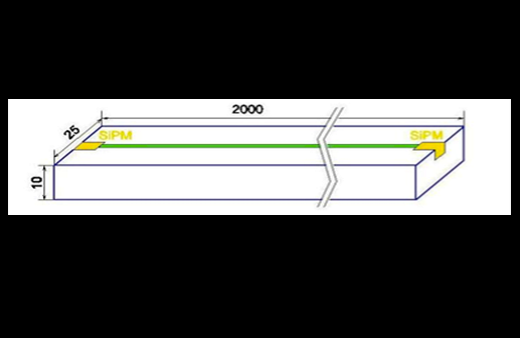
\includegraphics[width=0.4\hsize]{Detector/fig/muon_layer.png}
\end{tabular}
\caption{Iron yoke baseline structure (left) and scintillator instrumentation option (right).}
%\end{figure}
\label{fig:det:yoke}
%\begin{tabular}{cc}
\end{figure}

%\vspace{2cm}
\newpage
\section{Subdetector technology status}
\writer{Subdetector conveners}{}

%This section is one of the main technical added values of the IDR. It should summarize all technological progress since the DBD, including beam tests of technological prototypes and ongoing spinoffs. It should also indicate the remaining steps to fulfil the ILD requirements, with a focus of critical aspects associated to each technology choice. For conciseness only the highlights should be illustrated, with all details to be referenced in technical publications. As regards illustrations it is proposed to stick to o(1-2) photo and o(1-2) plot  for each technology. 

All ILD detector technologies under consideration have benefited from substantial developments since the DBD publication. Many activities are coordinated within worldwide R\&D Collaborations such as LCTPC [ref], CALICE [ref] or FCAL [ref]. Compared to the DBD studies, still focused on intrinsic physics response and performance, many technologies have now developed operational implementations 
with technological prototype which are mature for extrapolation to a full detector. This process has indeed already started with many spin-offs to existing experiments such as high-luminosity LHC detector upgrades. The experience gained with these applications will be a strong asset to the final design and construction of ILD.  


\vspace{1.0cm}

\subsection{Vertex detector}
%\writer{Auguste Besson, Akimasa Ishikawa, Marcel Vos}{3}

The vertex detector is a high-precision small device which is expected to be one of the latest subdetectors to be built and inserted within ILD. The development of optimal technologies can therefore proceed until a few years before the start of ILC. There has been much progress in this direction in the past 5 years for the three main options under consideration: CMOS, DEPFET and FPCCD sensors.

\subsubsection{CMOS sensors}

The use of CMOS sensors for particle physics has benefited a lot from the development in the past two decades of the MIMOSA chip series by the IPHC Institute. A first full scale particle physics detector application has been realized with the STAR vertex detector~\cite{Contin:2017mck} (Figure~\ref{fig:det:VTX_STAR}) on the RHIC hadron collider. Since then the technology has further developed as a widespread standard for pixel detectors, including many applications to e.g. LHC upgrades or new experiments. 

The general trend of performance improvements towards ILD specifications is summarized in table~\ref{ild:tab:CMOSdev}. Compared to STAR the new applications for the ALICE upgrade~\cite{AglieriRinella:2017lym} and CBM at FAIR~\cite{Koziel:2017loo} have moved to a technology with a smaller pattern, have implemented a new data driven readout scheme, and have improved the time resolution and power consumption to values close to ILD needs. The ALICE detector also concerns a very large area of more than 10 $m^2$, which qualifies the technology for the inner layers of a central tracker.

With these applications more attention is given to integration aspects of the technology. The chip intrinsic power consumption is now close to the ILD specification and could still be reduced by a factor $\simeq 10$ with power pulsing. To this respect a trade-off will have to be made between readout speed (related to time resolution) and power. With the expected heat production air cooling as done at STAR could be sufficient, but ILD has stronger constraints on the possible air flow due to a more forward instrumentation than STAR. This critical issue requires further studies. Low material ladder supports have been developed with the "PLUME" concept~\cite{Nomerotski:2011zz}, consisting in a thin foam layer carrying pixel chips on both sides as a double layer. First PLUME ladders have been built and a second version has been successfully operated for the BELLE II beam commissioning (Figure~\ref{fig:det:VTX_BELLE2} top).

\begin{table}\hspace*{-0cm}\small
\begin{tabular}{ l c c c c }
\toprule
DETECTOR: & STAR-PXL & ALICE-ITS & CBM-MVD & ILD-VXD \\
& (ULTIMATE) & (ALPIDE) & (MIMOSIS) & (PSIRA) \\
& 2014-16 & 2021-22 & 2021-22   & 2030 \\
\midrule
Technology (AMS): & 0.35 $\mu$m & 0.18 $\mu$m & 0.18 $\mu$m & $<$ 0.18 $\mu$m \\
Pixel size ($\mu$m$^2)$: & 20.7 x 20.7  & 27 x 29 & 22 x 33 & 22 x 22 or 18 x 18 \\
Readout mode:   & rolling shutter & data driven & data driven & data driven \\
Time resolution ($\mu$s):   & 135 & 5-10 & 5 & 1-4 \\
Power (mW/$cm^2$):   & 150 & 35  & 200  & 50-100 \\
Material ($X_0$/layer):   & 0.39\% & 0.3\%  &   & 0.15\% \\
\bottomrule
\end{tabular}
\caption{\label{ild:tab:CMOSdev}Development path of CMOS pixel sensors towards ILD.}
\end{table}



\begin{figure}[t!]
\centering
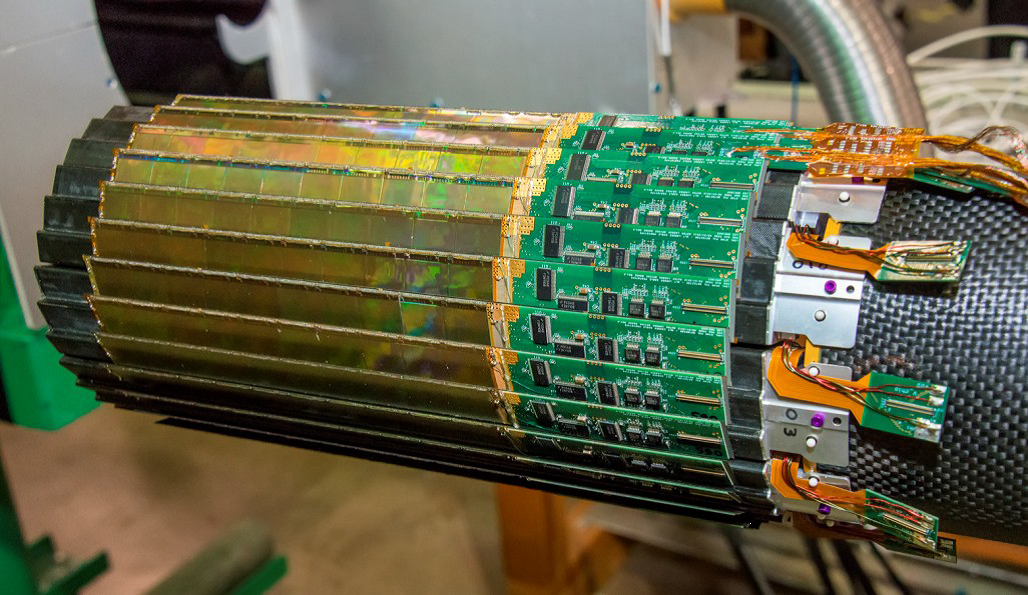
\includegraphics[width=0.6\hsize]{Detector/fig/VTX_STAR.png}
\caption{The vertex detector of the STAR experiment based on the "ULTIMATE" CMOS pixel sensor~\cite{Contin:2017mck}.}
\label{fig:det:VTX_STAR}
\end{figure}

\subsubsection{DEPFET sensors}

The development of DEPFET sensors in particle physics is reaching maturity. Following the demonstration of small
prototypes~\cite{Andricek:2011zza,Velthuis:2008zza} and first operational ladders five years ago the technology was 
chosen as the baseline for the vertex detector~\cite{Marinas:2011zz} of the Belle II experiment~\cite{Abe:2010gxa}. 
As many requirements of Belle II are similar to those
of the ILC, this can be seen as a 30\% prototype of the ILC vertex detector. DEPFET ladders have been successfully used 
in the BELLE II beam commissioning detector (BEAST 2). The first layer of the pixel vertex detector was installed in 2018
and is now in operation in the experiment (Figure~\ref{fig:det:VTX_BELLE2} bottom). Due to a low yield of the module assembly 
process, the second layer vertex detector is expected to be completed in 2020. While the experiment is 
taking data, studies towards future BELLE II upgrades based on advanced DEPFET technology are starting. The development of advanced DEPFET solutions for the ILD vertex detector is synergetic with this effort.

\begin{figure}[t!]
\centering
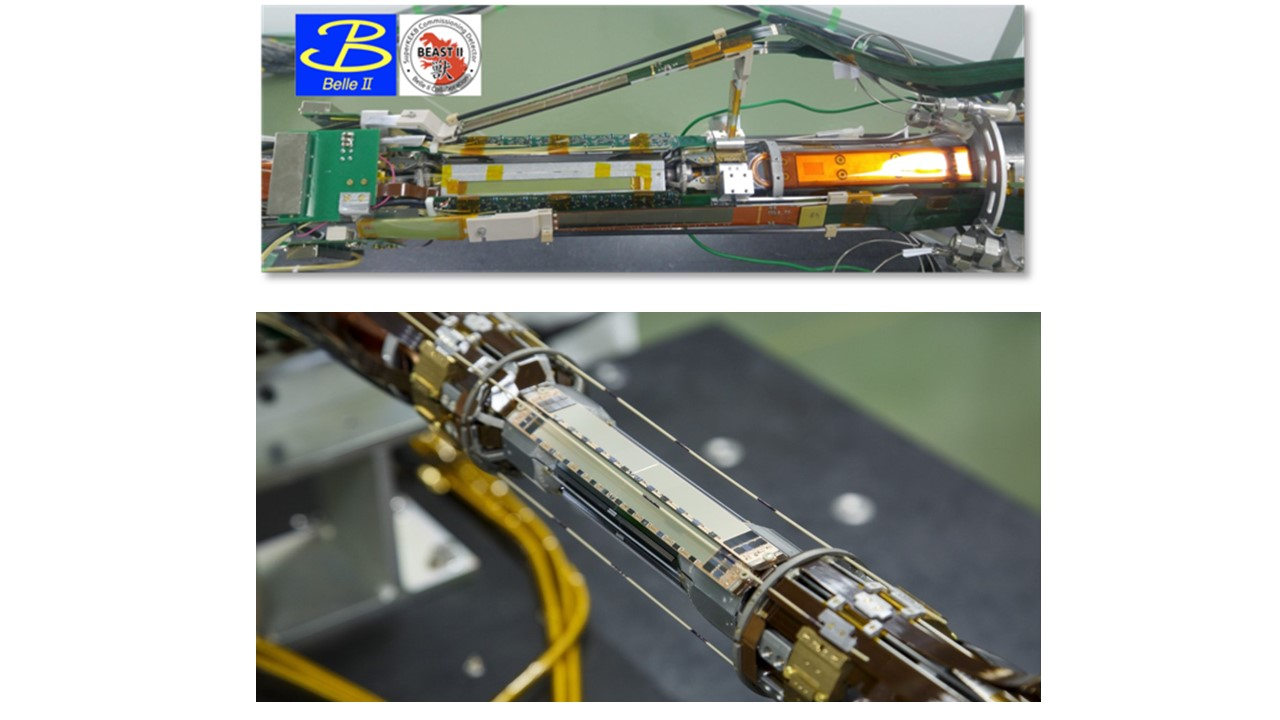
\includegraphics[width=1.0\hsize]{Detector/fig/VTX_BELLE2.jpg}
\caption{Pixel detectors of the BELLE II experiment. Top: beam commissioning with "PLUME" CMOS (inclined sensors) and DEPFET (barrel) ladders. Bottom: the BELLE II DEPFET vertex detector.}
\label{fig:det:VTX_BELLE2}
\end{figure}

\subsubsection{FPCCD sensors}

The FPCCD technology is not yet used in full size detector applications but a first large prototype has been built~\cite{ild:bib:FPCCD} with a sufficient size to cover the inner layer of the ILD vertex detector. The prototype is currently undergoing detailed characterization with e.g. radioactive source signals (Figure~\ref{fig:det:VTX_FPCCD}). Irradiation tests of FPCCDs are also being performed since radiation hardness is a critical aspect of this technology.   

\begin{figure}[t!]
\centering
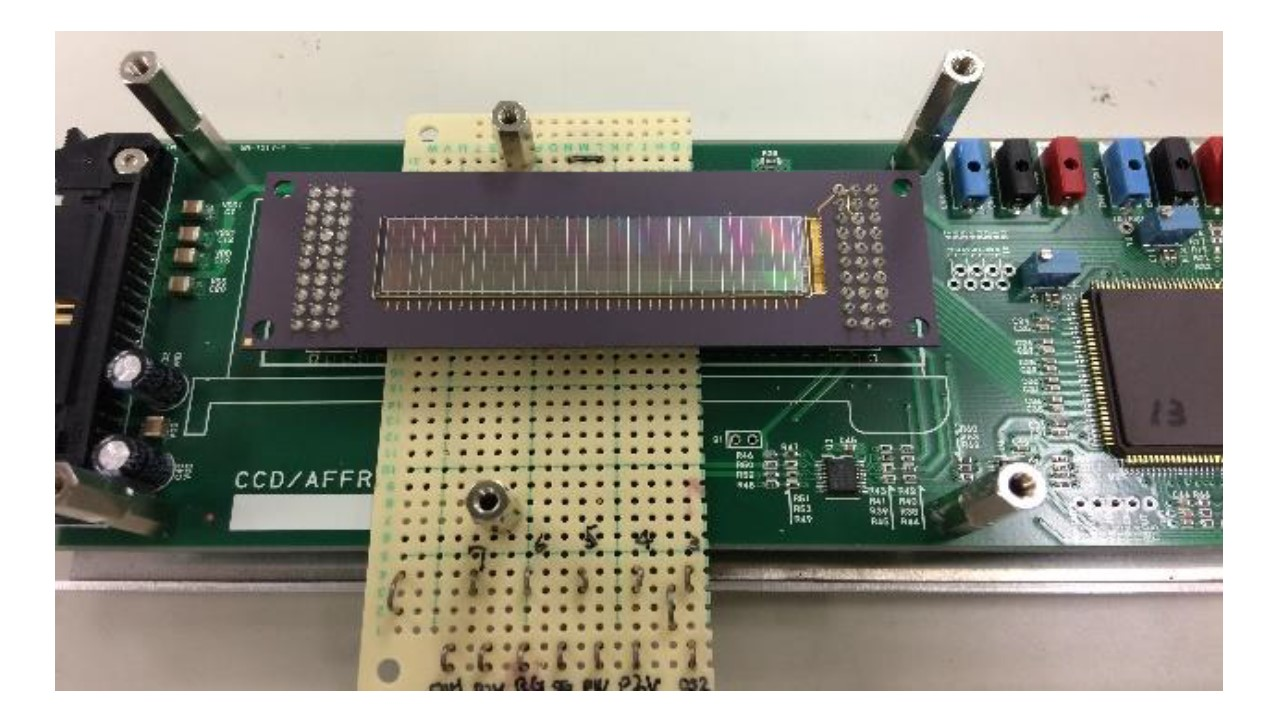
\includegraphics[width=0.6\hsize]{Detector/fig/VTX_FPCCD.jpg}
\caption{First full size FPCCD ladder on its test bed.}
\label{fig:det:VTX_FPCCD}
\end{figure}

\vspace{2cm}
\subsection{Silicon trackers}
\writer{(Besson, Vos, Vila)}{3}

The silicon sensors surrounding the vertex detector will directly benefit from the previous pixel detector R\&D as regards their high-spatial resolution components. In the past years the specific silicon R\&D has focused around two lines: a generic development of high-resolution timing sensors, and the prototyping of mechanical support structures of the Forward Tracking Detector.

\subsubsection{ILGADs for precise tracking and time stamping (4D-tracking)}

The Low Gain Avalanche Detector (LGAD) is the baseline sensing technology of the recently proposed Minimum Ionizing Particle (MIP) end-cap timing detectors (MTD) at the Atlas and CMS experiments. LGADs are n-on-p silicon detectors with an internal gain. To obtain this gain, an extra, highly doped, layer is added just below the p-n junction of a PIN diode. This highly doped region creates a very high electric field region. This electric field induces an avalanche multiplication of the electrons and thus create additional electron-hole pairs\cite{PELLEGRINI201412}. 

The current MTD's sensor is designed as a multi-pad matrix detector delivering a poor position resolution, due to the relatively large pad area, around 1 $mm^2$; and a good timing resolution, around 20-30 ps. Besides, in his current technological incarnation, the timing resolution of the MTD's LGAD sensors is severely degraded once the MIP particle hits the inter-pad region since the signal amplification is missing for this region. This limitation is named as the LGAD fill-factor problem. For the ILD, a true 4D tracking  must overcome the poor spatial resolution and fill factor limitations. A new p-in-p LGAD architecture named as inverse LGAD (iLGAD) tackles both issues\cite{Carulla_2016}. Contrary to the conventional LGAD design, the iLGAD has a non-segmented multiplication layer, and it should ideally present a constant gain value over all the sensitive region of the device without gain drops between the signal collecting electrodes, see figure\,\ref{fig:det:cross-section}. This feature has been experimentally confirmed on a strip-like segmented iLGAD and compared against a conventional strip-like LGAD and PIN devices\cite{Curras2019}. 

\begin{figure}[t!]
\centering
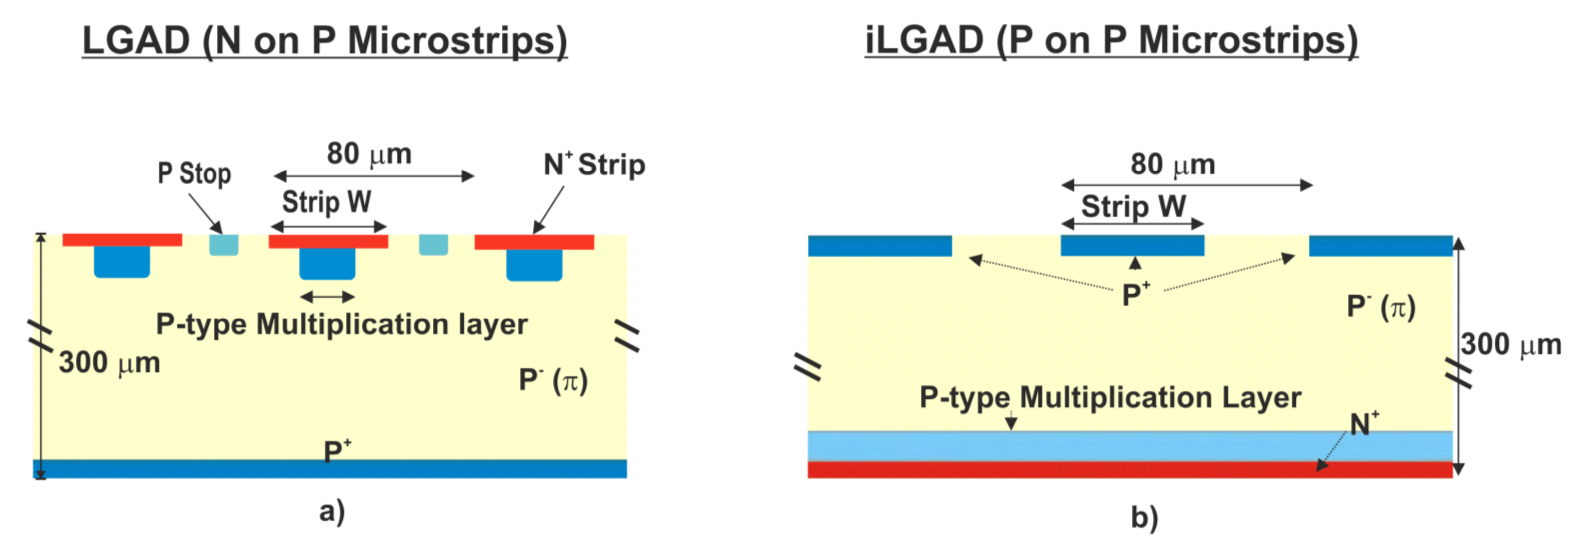
\includegraphics[width=0.6\hsize]{Detector/fig/cross-section.png}
\caption{Cross-sections of the core layout of LGAD (left) and iLGAD (right) microstrip designs.}
\label{fig:det:cross-section}
\end{figure}

The tracking performances of one LGAD and one iLGAD strip detector manufactured at IMB-CNM were studied in a test beam at CERN-SPS and compared with a standard PIN strip detector. These three strip detectors were unirradiated and consisted of 45\,strips with a 160\,$\mu$m pitch. 
The big advantage of the iLGAD technology was confirmed during the test beam. It was proved that while in the LGAD strip detector the signal is severely degraded in the inter-pad region, the iLGAD presents a very constant gain value over all the sensitive region of the device. These results are shown on figure\,\ref{fig:det:fill-factor}. The charge distribution of the LGAD measured during the test beam presents two peaks: one around 24\,ke, corresponding to the MIP particles that cross the interstrip region where the generated signal is not amplified (same charge measure in the PIN strip); and one around 77\,ke, corresponding to the particles that cross the region where the signal is amplified. On the other hand, the same plot produced for the iLGAD detector presents only one peak in the charge distribution around 75\,ke. In this case,  the signals produced for all MIP particles that cross the sensitive region of the device are amplified, resulting in a much better and uniform response along the sensitive region. The tracking and timing performances were also quantified during the test beam: they achieve values of tens of microns and picosenconds, respectively.


\begin{figure}[t]
\centering
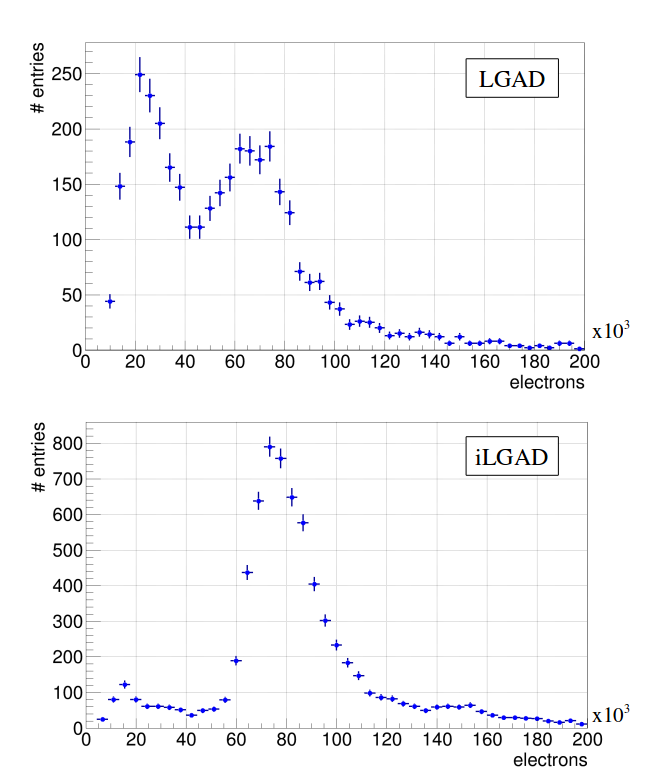
\includegraphics[width=7cm]{Detector/fig/fill-factor.png}
\caption{Charge distribution measured during the test beam for one LGAD strip detector (top) and one iLGAD strip detector (bottom). The fill-factor problem visible for the LGAD case is not present in the iLGAD structure.} 
\label{fig:det:fill-factor}
\centering
\end{figure}


\subsubsection{Thermo-mechanical studies of the FTD support structure}

The combination of the requirements of minimal material and a mechanical stability to 
the level of several $\mu\mathrm{m}$ represents quite a challenge. A realistic, 
full-scale mechanical prototype of the disks has been developed to characterize 
its thermo-mechanical performance 
in conditions that resemble those of the experiment (Figure~\ref{fig:det:FTD_mockup}). 
This {\em mock-up} is based on a Carbon-fibre support disk
and 50~$\mu\mathrm{m}$ thick silicon petals designed at IFIC Valencia. 

%% add Malte and Maria to author list?
The Carbon fibre disks were produced by INTA in Madrid. It consists of
a 1 mm thick rohacell core covered on both sides by three-layer carbon fibre skins. The 
resulting structure adds less than XXX \% of a radiation length ($X_0$) to the material 
budget. The mounting points for the Silicon sensors are formed by precisely machined 
PEEK inserts that are glued into the Carbon fibre structure. The gluing procedure controls
the relative position of the mounting points to better than 50 $\mu \mathrm{m}$ with
a custom jig. 

The Silicon petals were produced at the HalbLeiterLabor of the Max Planck Society in 
Munich (MPG-HLL) using the Silicon-on-Oxide process that is at the heart of the
all-silicon-ladder concept~\cite{Andricek:2004cj}. The 50 $\mu \mathrm{m}$ thick sensor 
area is supported by a 500 $\mu \mathrm{m}$ thick rim.

The contribution to the material budget of the sensors and support disks is 
summarized in Table~\ref{tab:ftd_disk_material_budget}. The Silicon sensors clearly
dominate the total contribution.

\begin{table}[]
    \centering
    \begin{tabular}{l|c|c}
    Component                      & material (\% $X_0$) \\ \hline
    Silicon petals                &                   \\
    Carbon fibre (incl. cyano-ester resin)     &   0.038 \\
    Honeycomb core (Aramide)      &   0.0006 \\
    PEEK inserts                  &   0.0019 \\
    PEEK screws                   &   0.0014 \\
    glue                          &   0.0006  \\ \hline
    total                         &           \\ \hline
    \end{tabular}
    \caption{Contribution to the material bugdet of the Forward Tracking Disks. The contributions are determined for perpendicular incidence and average over the area
    of the disk.}
    \label{tab:ftd_disk_material_budget}
\end{table}

The thermo-mechanical performance of the loaded disk has been tested extensively. The 
support disk is found to have a planarity of 200 $\mu \mathrm{m}$ (RMS). Despite the 
minimal material it is very stiff, with an eigenfrequency greater than 1 $kHZ$. The
silicon petals are mounted kinematically, such that are free to expand in response
to a thermal load, while distortions of the sensors out of the nominal plane remain
very tightly constrained. The torque applied to the screws must be carefully 
chosen: a torque of 3 $mN \cdot m$ is found to be optimal. 
With this choice, the first eigenfrequency of a free petal (167 $Hz$) is nearly
doubled (to $\sim$ 270 $Hz$) when the sensor is clamped to the disk 

The impact of air cooling on the mechanical stability is studied with a local, 
laminar air flow. The power consumption pattern mimics that of a DEPFET
active pixel detector, assuming that the application of power pulsing reduces
the average power consumption by a factor 20.
In these conditions, a gentle, laminar flow of 1 $\mathrm{m/s}$ is found to be sufficient
to keep the temperature gradient over the sensor to within 10 degrees C, 
Vibrations due to air flow have an  amplitude of less than 1 $\mu \mathrm{m}$ 
for laminar air flow with a velocity up to 4 $\mathrm{m/s}$. 

These results indicate that an aggressive design based on a thin Carbon fibre
support disk and ultra-thin self-supporting Silicon petals can meet the 
stringent requirements on mechanical stability of the ILD experiment.





\begin{figure}[t!]
\centering
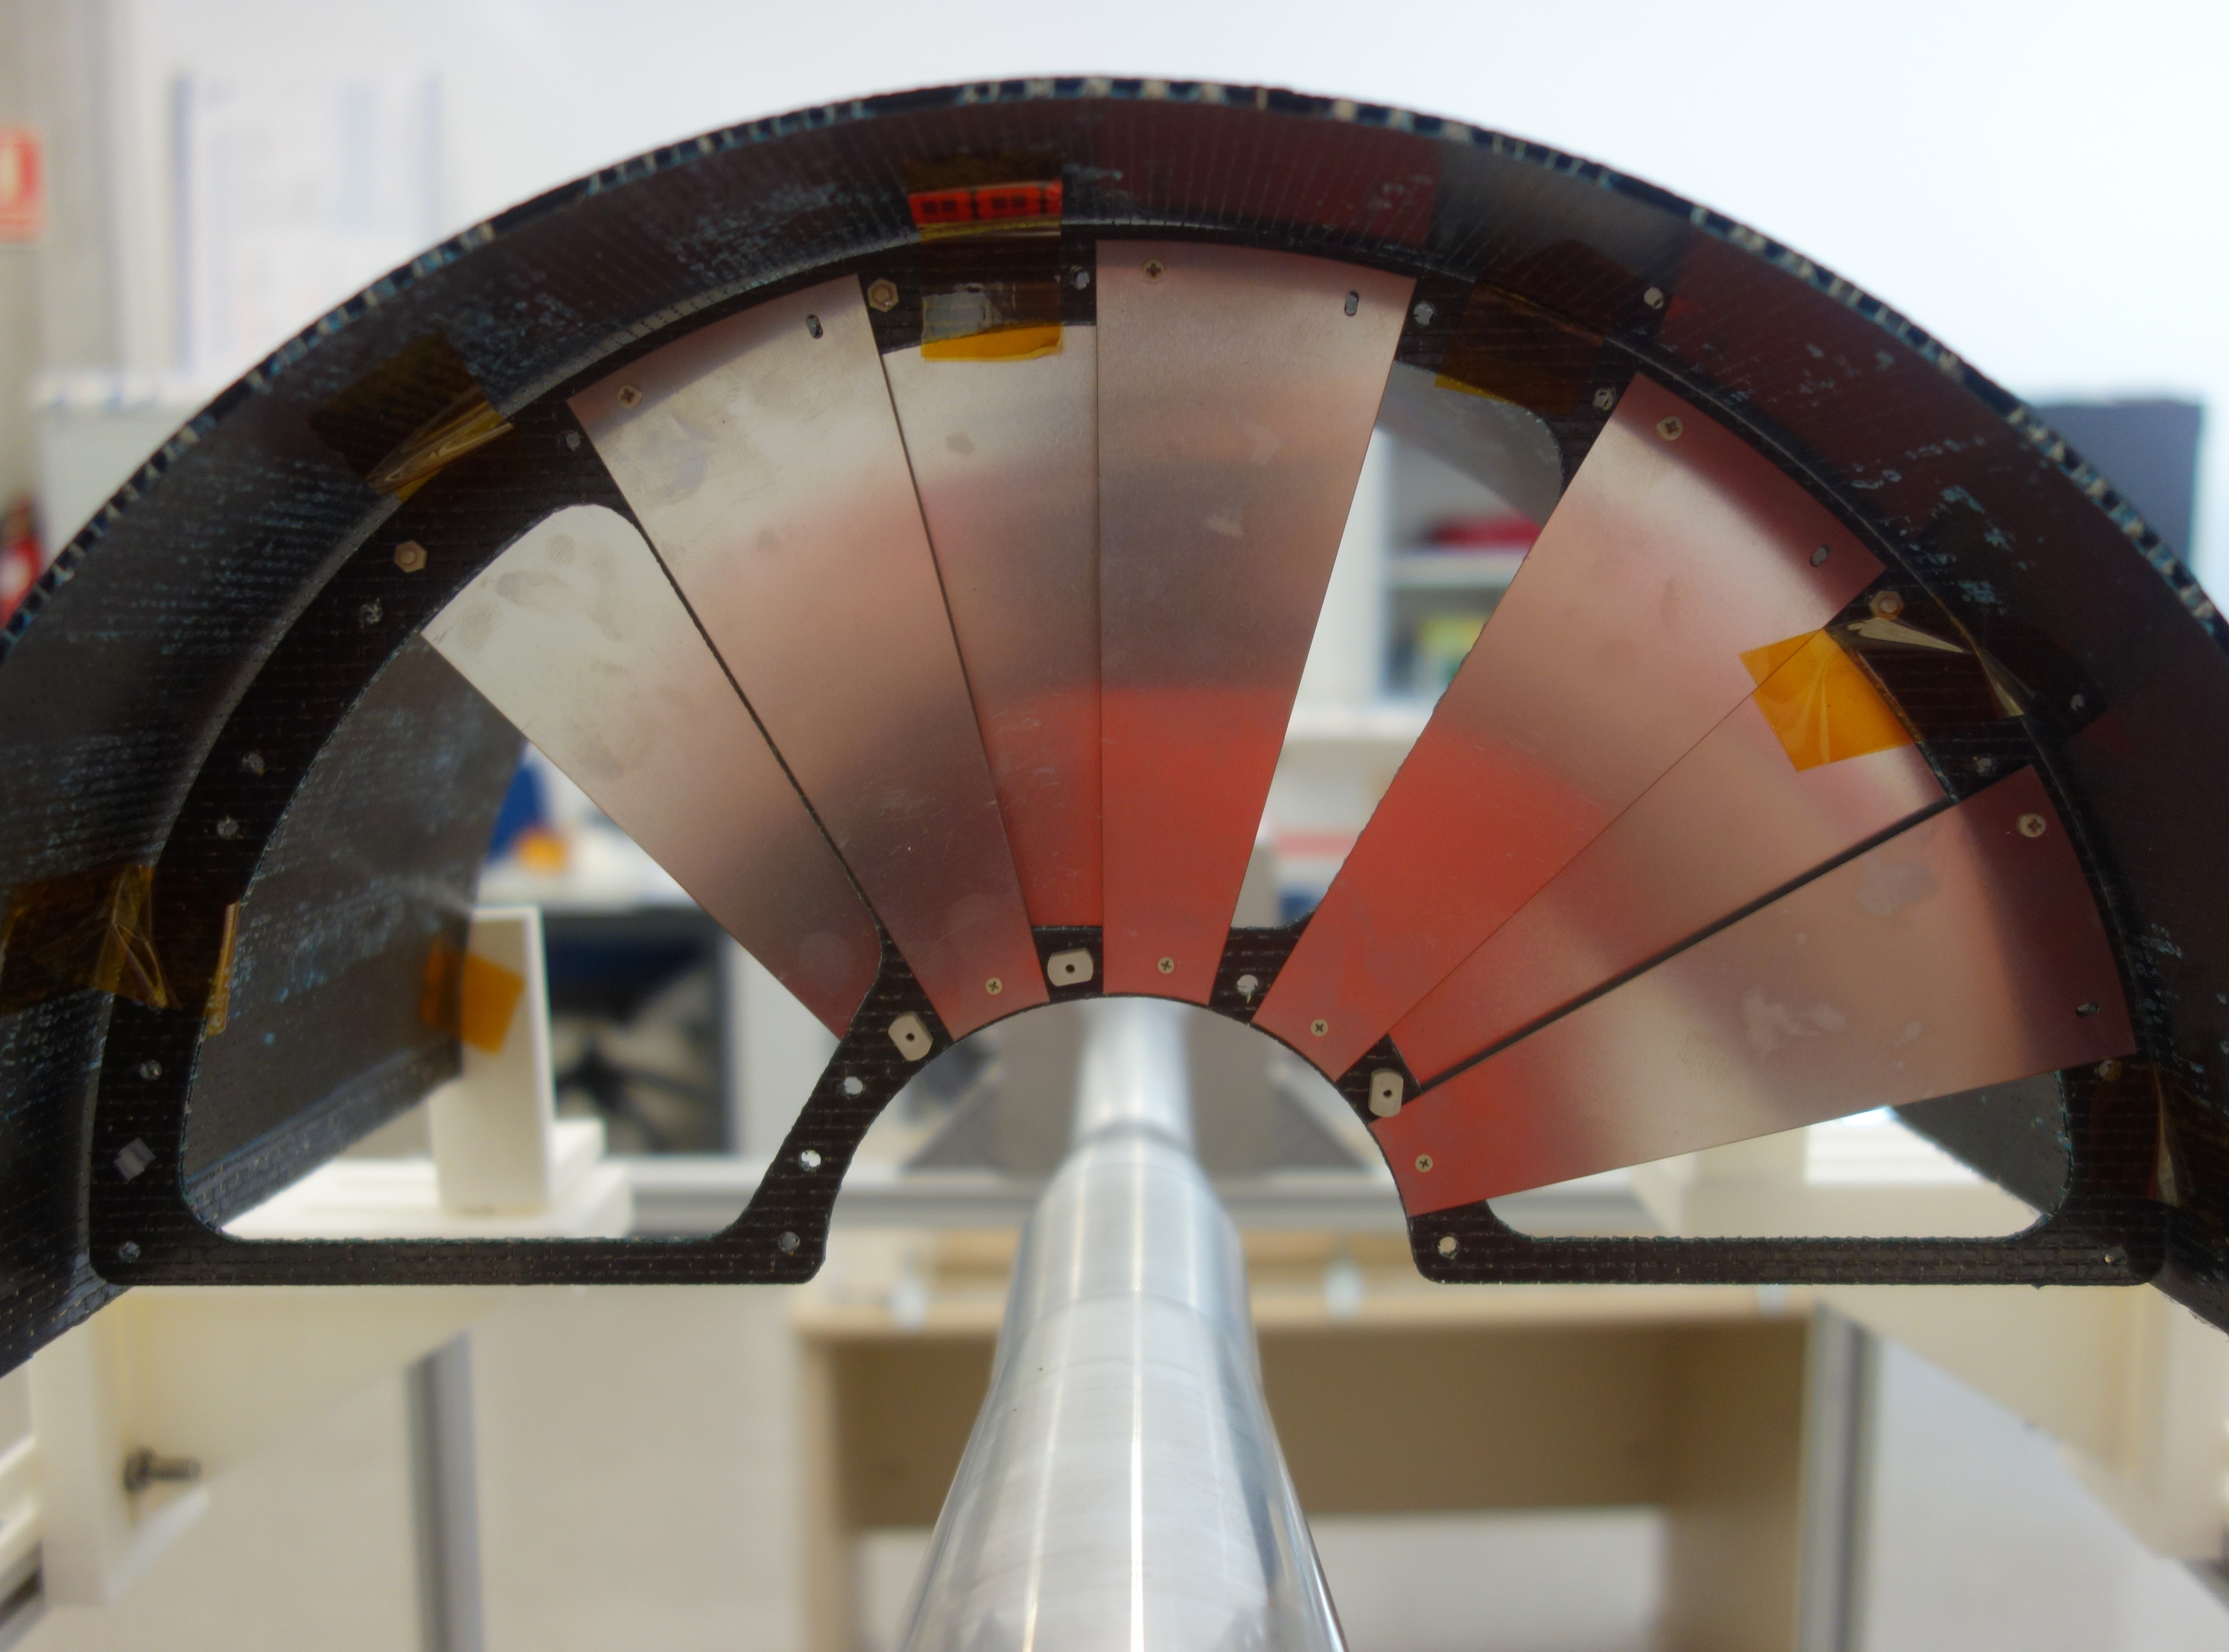
\includegraphics[width=0.6\hsize]{Detector/fig/FTD_mockup.jpg}
\caption{FTD thermo-mechanical mockup for the 2 inner disks.}
\label{fig:det:FTD_mockup}
\end{figure}


\vspace{2cm}

\subsection{Time Projection Chamber}
%\writer{Paul Colas, Akira Sugiyama}{3}

The ILD TPC R\&D is being conducted mainly within the LCTPC Collaboration \cite{ild:bib:TPC_lctpc}. The history of these developments is described in the R\&D liaison report of the Linear Collider Collaboration~\cite{ild:bib:TPC_liaison} which contains many references (pp 36-60).

The workhorse for validation of detector prototypes and operational conditions is the TPC test set-up installed permanently in the DESY test beam~\cite{ild:bib:TPC_desytb} (Figure~\ref{fig:det:TPC_test_setup}). The TPC is situated in a superconducting magnet providing a magnetic field of 1 Tesla, and the beam line is equipped with precise incident and outgoing particle beam telescopes allowing to quantify the TPC reconstruction precision as function of the particle parameters. The beam test set up is currently being upgraded with the high precision LYCORIS silicon telescope~\cite{ild:bib:TPC_lycoris}, and a new TPC field cage with reduced field distortion is being assembled.

\begin{figure}[t!]
\centering
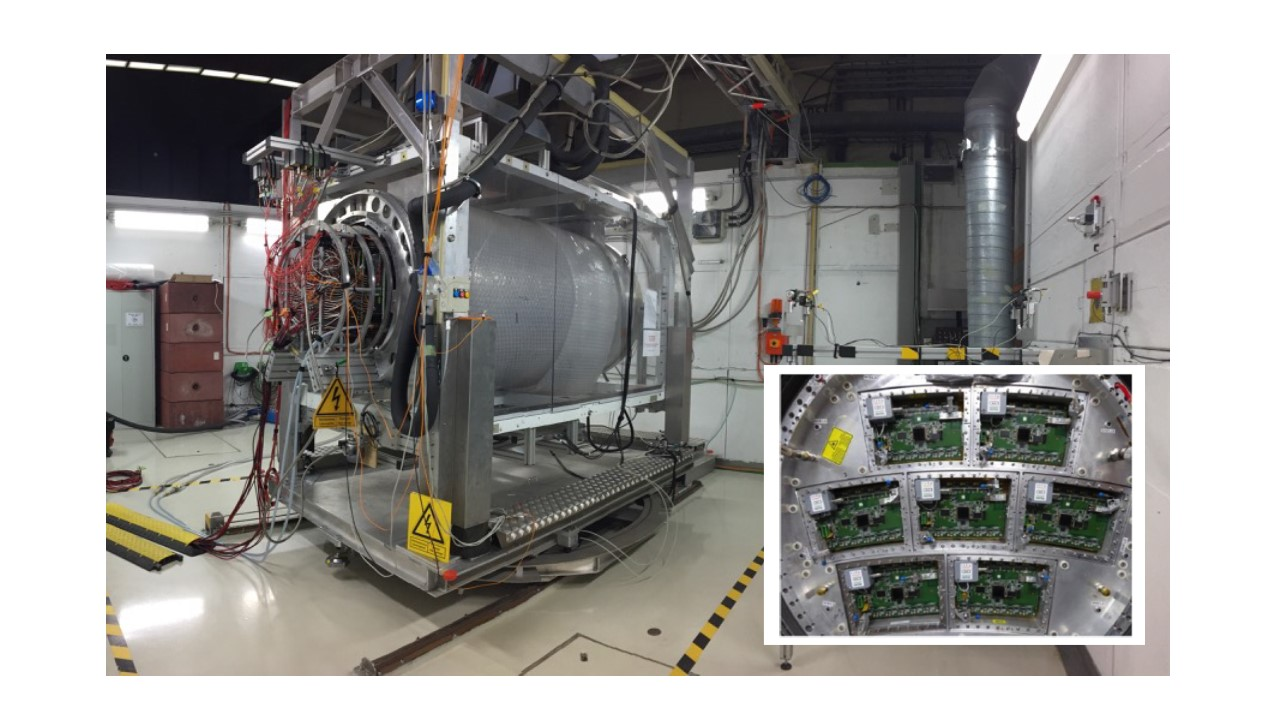
\includegraphics[width=1.0\hsize]{Detector/fig/TPC_test_setup.jpg}
\caption{The TPC test setup at DESY. The insert shows the geometrical structure of the TPC end cap which can host prototypes of detection planes.}
\label{fig:det:TPC_test_setup}
\end{figure}

Significant progress has been seen in the manufacturing process of detection modules for each of the readout options. A new Micromegas layout with resistive anodes has been shown to exhibit reduced boundary distortions~\cite{ild:bib:TPC_distortions}. The flatness of the GEM modules has been improved significantly, increasing the gain uniformity by a factor 2~\cite{ild:bib:TPC_GEMflatness}. Operational GridPix "QUAD" modules have been built based on the TimePix3 pixel chip~\cite{ild:bib:TPC_quad}. Recent prototypes of the three types of detection modules are shown in Figure~\ref{fig:det:TPC_prototypes}.  

\begin{figure}[t!]
\centering
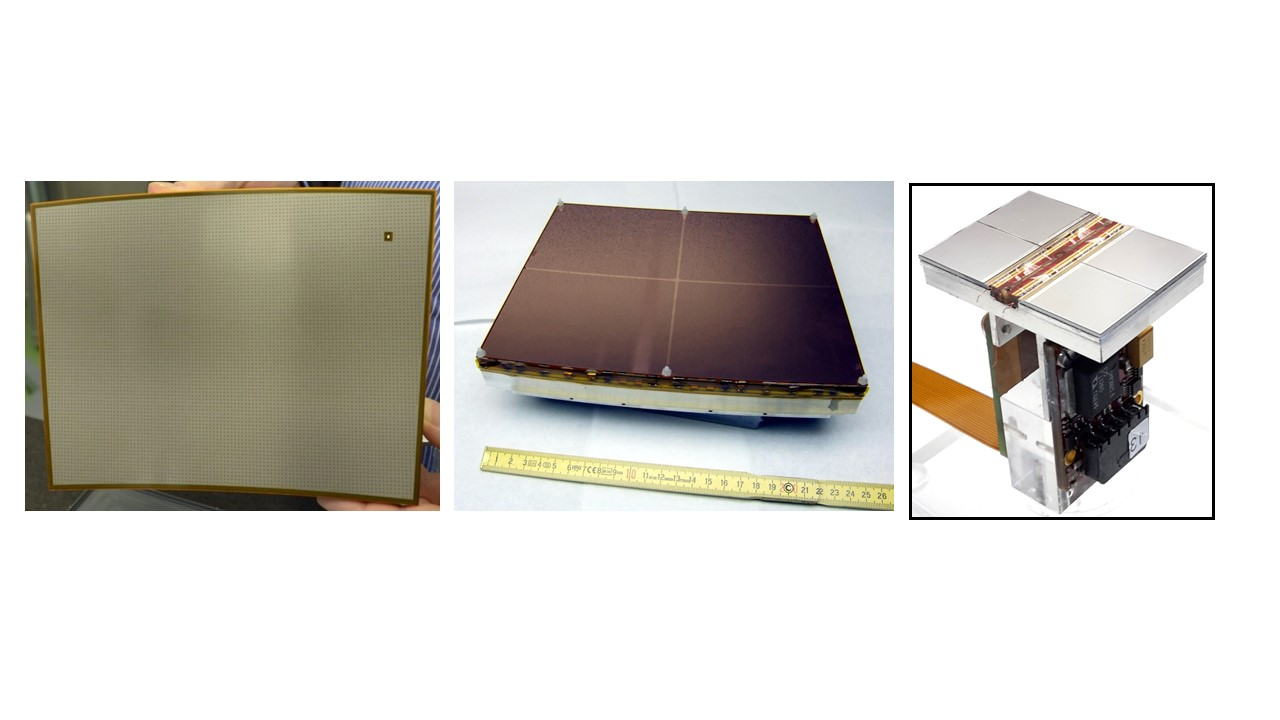
\includegraphics[width=1.0\hsize]{Detector/fig/TPC_prototypes.jpg}
\caption{TPC prototype detection modules for the three baseline technologies under consideration: Micromegas module (left), GEM module (middle) and GridPix QUAD module (right).}
\label{fig:det:TPC_prototypes}
\end{figure}

The performance of the three technologies has been measured in beam tests. Figure~\ref{fig:det:TPC_performances} shows the measured point resolution in 1~T magnetic field for drift distances from 0 to 0.6 m. This can be safely extrapolated to $\sim~100$ $\mu$m in a field of 3.5~T at a drift length of 2.3~m: the higher magnetic field reduces the transverse diffusion constant in the selected gas from 91~$\mu \mathrm{m} / \sqrt{\mathrm{cm}}$ to 30 $\mu \mathrm{m} / \sqrt{\mathrm{cm}}$, which compensates for the longer drift length compared to the prototype set-up. The dE/dx resolution determined by the truncated mean method has been measured to be $4.6\%, 4.5\%$ and $4.2\%$, respectivly, for Micromegas, GEM and GridPix technologies. It improves to $3.8\%$ for GridPix using a cluster counting method. The conclusion is that the target requirement of a spatial resolution of 100 microns and an aim of a dE/dx resolution better than 5\% have been reached in all cases.   
\begin{figure}[t!]
\centering
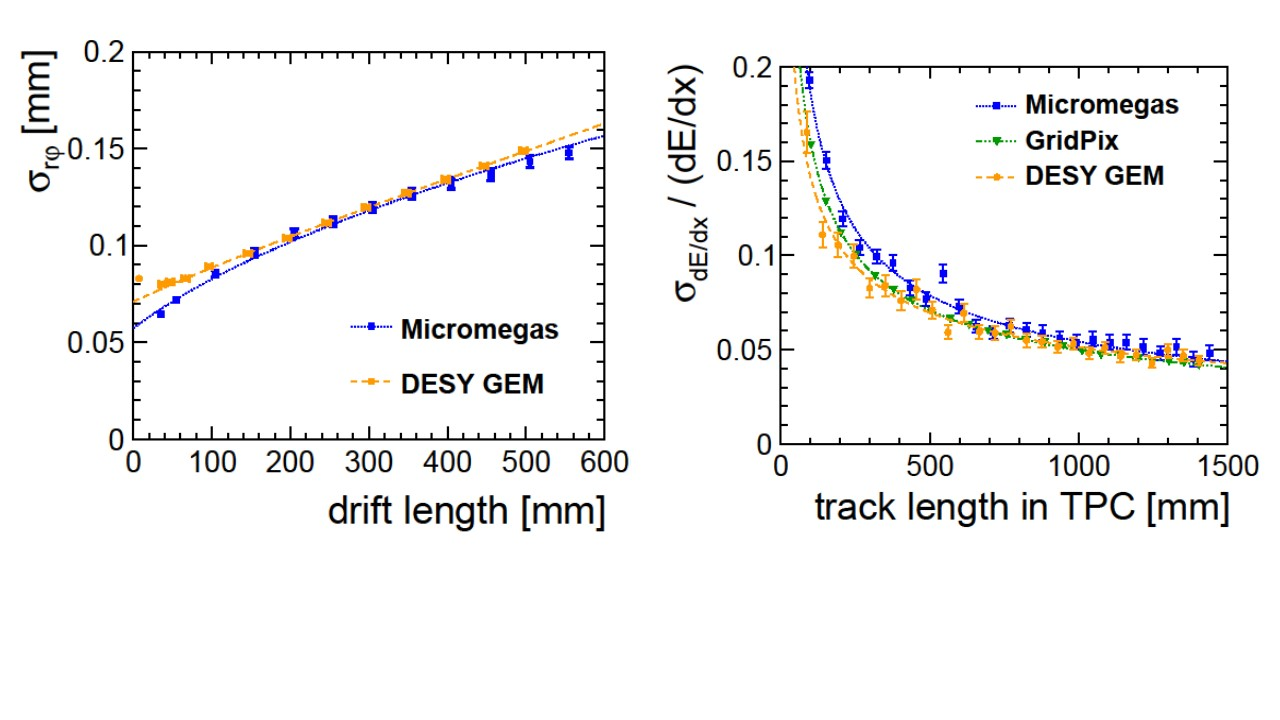
\includegraphics[width=1.0\hsize]{Detector/fig/TPC_performances.jpg}
\caption{Resolution on the track position in r$\phi$ (left) as function of the drift length and resolution on the ionisation loss dE/dx (right) as function of the track length, for the three readout options under consideration.}
\label{fig:det:TPC_performances}
\end{figure}

Two-track separation has also been investigated. A $47\%~\rm{X_0}$ steel target was introduced near the TPC wall to produce multi-track events suitable for this study.
From these events a 2-hit separation distance of 4 to 6~mm was measured depending on the drift distance. An algorithm based on fitting the double-hit charge deposition with expected pad response function width allowed this separation distance to be reduced to 2~mm, with 1.3~mm pads (Figure~\ref{fig:det:TPC_separation}).

\begin{figure}[t!]
\centering
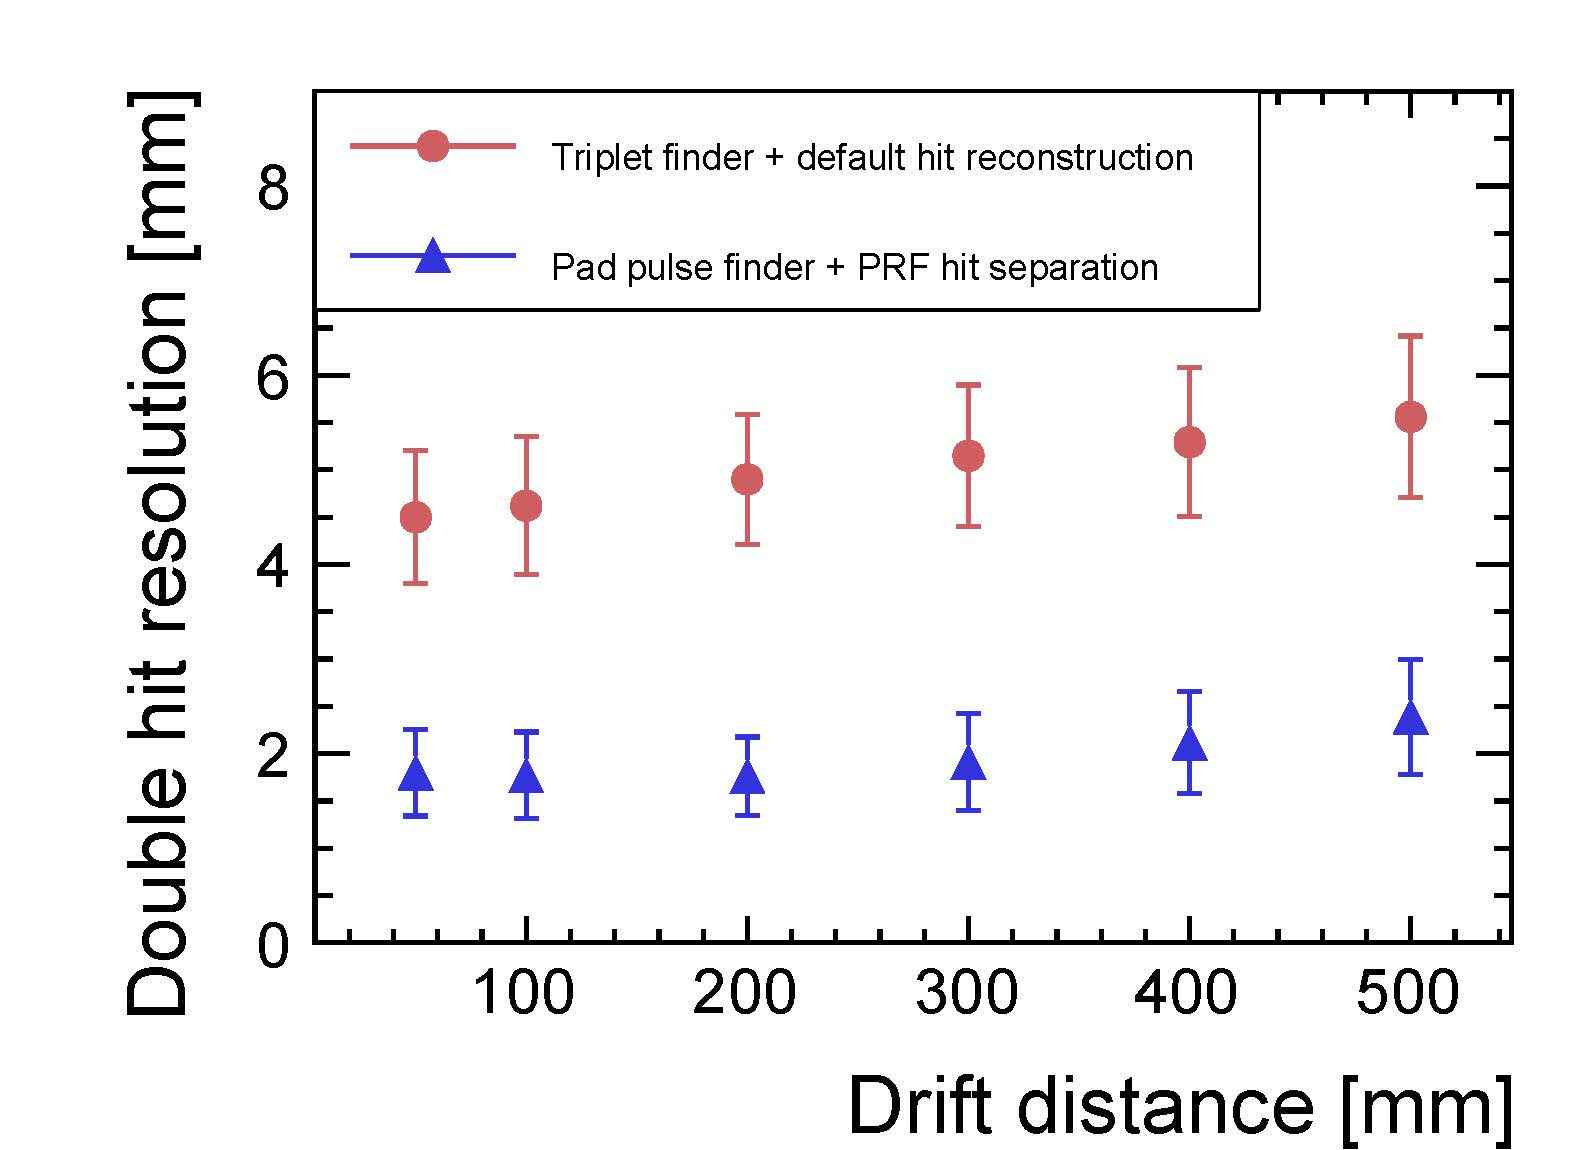
\includegraphics[width=0.7\hsize]{Detector/fig/TPC_separation.jpg}
\caption{2-hit separation as a function of the drift distance from beam test. Red dots are the results for standard hit reconstruction. Blue triangles show the results of the improved algorithm}
\label{fig:det:TPC_separation}
\end{figure}

A critical aspect of the TPC operation consists in the cooling of the readout end-caps, which must be realised with minimal dead material.  For this a double phase $\mathrm{CO}_2$ cooling system with thin low-material fluid pipes has been developed and shown to perform adequately. 

Also critical for ultimate performance is the mitigation of the drift field distortions which may develop from the accumulation of ions in the drift volume. For this an ion gating scheme based on a large aperture GEM foil (Figure~\ref{fig:det:TPC_gating} left) has been implemented and beam tested~\cite{ild:bib:TPC_gatinginbeam}. To prevent the positive ions created by the avalanches in the amplification device from flowing back to the drift space, a counter-field is created by applying a polarisation $\Delta V$ of -20 V between the faces of the gating GEM foil in between beam train crossings. During train crossings the voltage difference is reversed to +3 V, opening the way to the incoming electrons to be multiplied. 

Results from test bench measurements show that a good transparency for drift electron signals can be maintained while reducing the accumulation of ions in the drift volume by one order of magnitude~\cite{ild:bib:TPC_gatingpaper} (Figure~\ref{fig:det:TPC_gating} right).

\begin{figure}[t!]
\centering
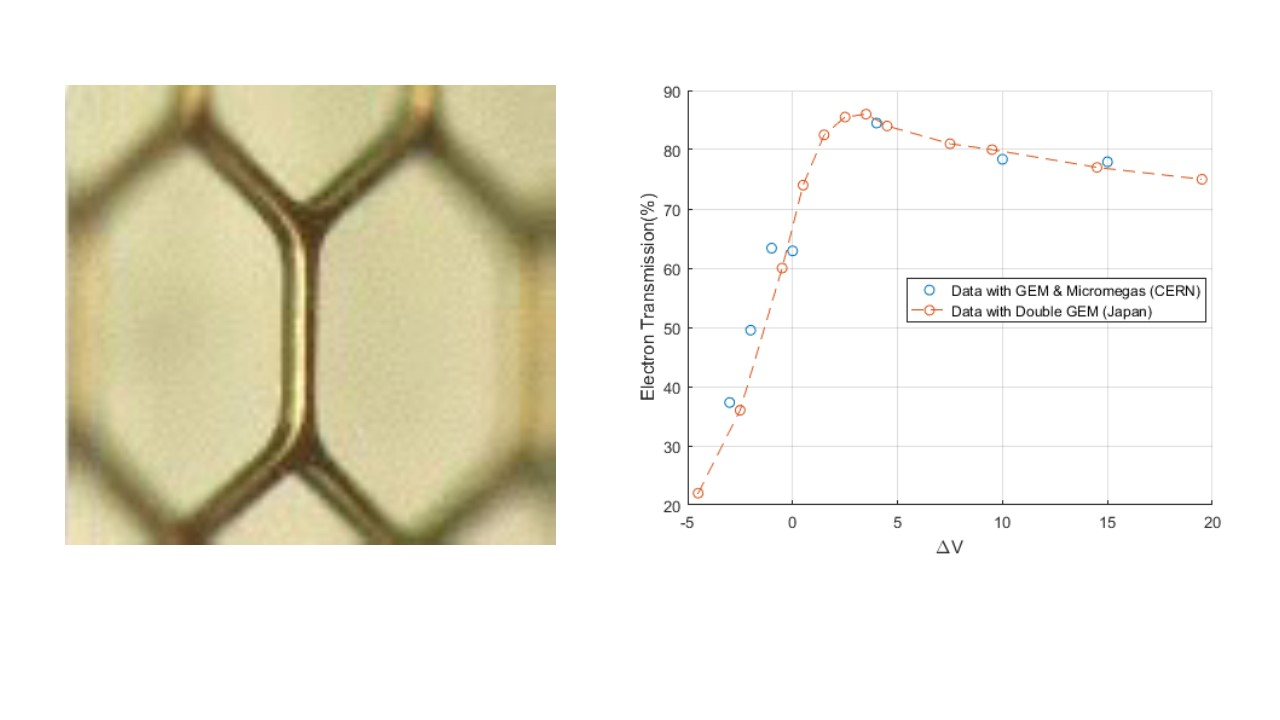
\includegraphics[width=1.0\hsize]{Detector/fig/TPC_gating.jpg}
\caption{TPC gating: detail of a GEM gating grid (left) and signal electron transparency with GEM gating as a function of the voltage difference (in Volts) across the two sides of the GEM plane in gate open mode (right).} 
\label{fig:det:TPC_gating}
\end{figure}

In conclusion all basic aspects of the operation have shown to meet the requirements for an experiment at the ILC. 
\subsection{Electromagnetic Calorimeter}
%\writer{Jean Claude Brient, Wataru Ootani}{3}

\subsubsection{Silicon option (SiECAL)}

In the past 5 years the Silicon option of the electromagnetic calorimeter has focused on the design and construction of technological prototypes of the detector including beam tests. The current technological developments have led to choosing 20cm wafers for making the diode matrices, with a standard thickness of up to 725 micrometers. When applied to ILD this would result in a slightly thicker EM calorimeter than foreseen in the baseline design, and is one of the motivations to reduce the numbers of layers from 30 to 26 (see section 5.1.2).

A fully integrated layout of the detection board has been designed with the required dimension of 16 x 16 $cm^2$ corresponding to 1024 channels (Figure~\ref{fig:det:SiWECAL_proto} top). The board hosts 16 SKIROC ASICs developed by OMEGA~\cite{Callier:2011zz,Suehara:2018mqk} to process 64 channels each. A calorimeter prototype based on 10 such detection layers has been built~\cite{Boudry:2014bxa,Poeschl:2015jma} (Figure~\ref{fig:det:SiWECAL_proto} bottom) and beam-tested on several occasions at DESY and CERN, including a combined test with a SDHCAL prototype of the hadronic calorimeter (next section).   
\begin{figure}[t!]
\centering
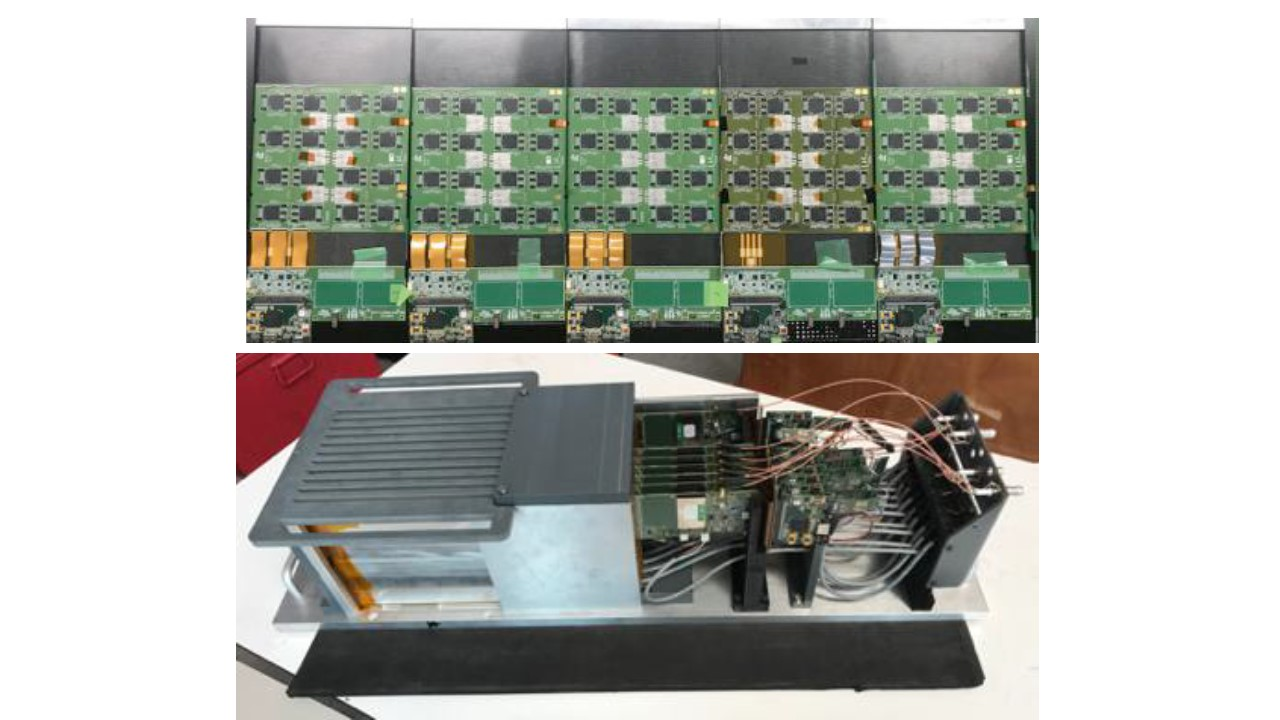
\includegraphics[width=1.0\hsize]{Detector/fig/SiWECAL_proto.jpg}
\caption{Technological prototype of the SiECAL. Top: set of integrated sensor\&readout boards; bottom: 10-layers calorimeter prototype used in beam tests at DESY and CERN.}
\label{fig:det:SiWECAL_proto}
\end{figure}

The response of this technological prototype to particles behaves as expected~\cite{Kawagoe:2019dzh}. A signal-to-noise ratio of 20 is measured for MIPs in single pads (Figure~\ref{fig:det:SiWECAL_signals} left). Such a large signal/noise ratio of MIPs is important for isolated particle identification in particle flow energy reconstruction. First response to high energy electrons has recently been measured at CERN in a combined test with the SDHCAL (Figure~\ref{fig:det:SiWECAL_signals} right). The beam tests have also been used to validate the power pulsing of the front-end electronics required to minimize heat production within the calorimeter. A new version of the detector slabs is currently in production from a joint development in LLR and Kyushu. A total number of 20 detection layers could be reached in the coming year. This will allow the construction of a full ECAL prototype to be used in test beams for measurements of the energy resolution.

\begin{figure}[t!]
\centering
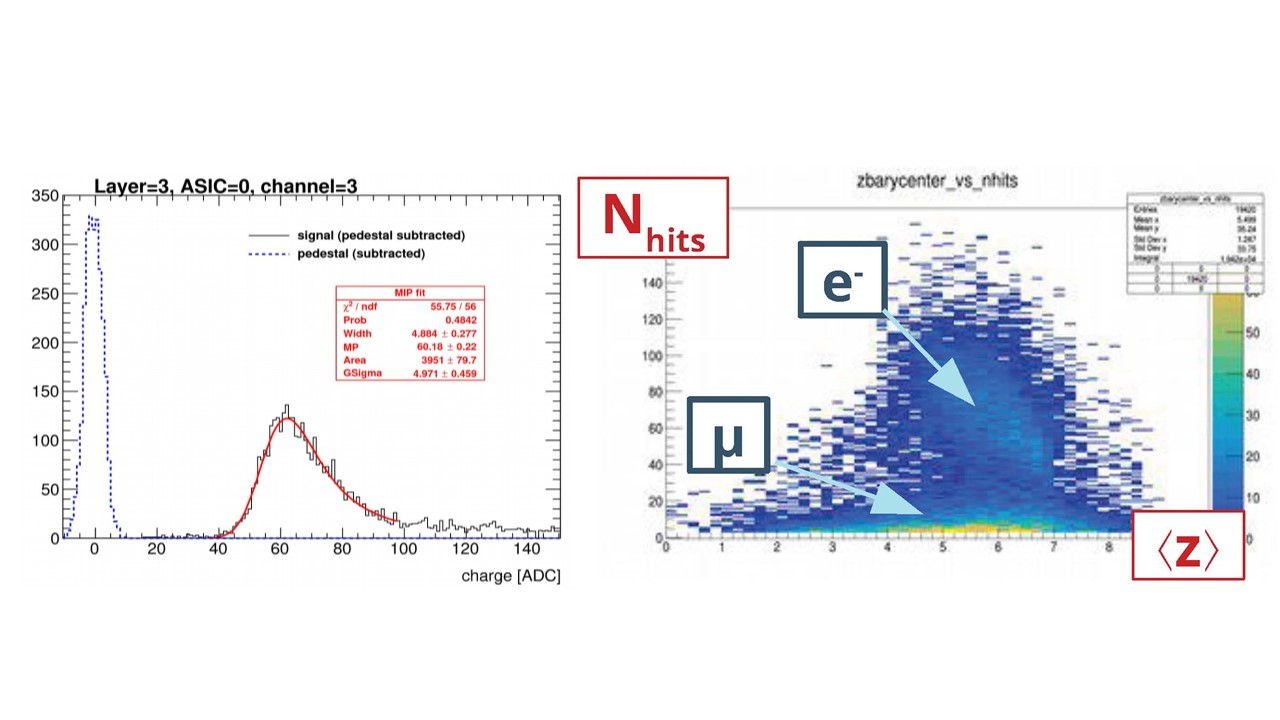
\includegraphics[width=1.0\hsize]{Detector/fig/SiWECAL_signals.jpg}
\caption{Particle response of the SiECAL prototype: MIP response of a single pad (left) and shower profile of muons and 80 GeV electrons (right).}
\label{fig:det:SiWECAL_signals}
\end{figure}

More developments are ongoing to reach the requirements of the full-size ILD detector. The layout of the sensitive layer diode matrices has been revisited since the technological prototype construction. A large detector slab with dimensions similar to those of the calorimeter modules has been built and tested with MIPs~\cite{Balagura:2017vvf} (Figure~\ref{fig:det:SiWECAL_dev} right). A 10\% signal drop has been observed along the full length of the slab and could be attributed to power voltage drops and clock reflections. An updaded long slab is under construction to correct these effects and validate the solutions. In addition, an electronics readout concentrator and interface board with the detector slabs, located at the end of the slabs, is under development in LAL with a size and performance close to those needed for the ILD detector. Ultra thin detection boards with ASICs integrated within the PCB have also been developed and are under test with cosmics (Figure~\ref{fig:det:SiWECAL_dev} left). Provided industrial aspects are under control, they may allow even more compact layouts of the electromagnetic calorimeter. 

\begin{figure}[t!]
\centering
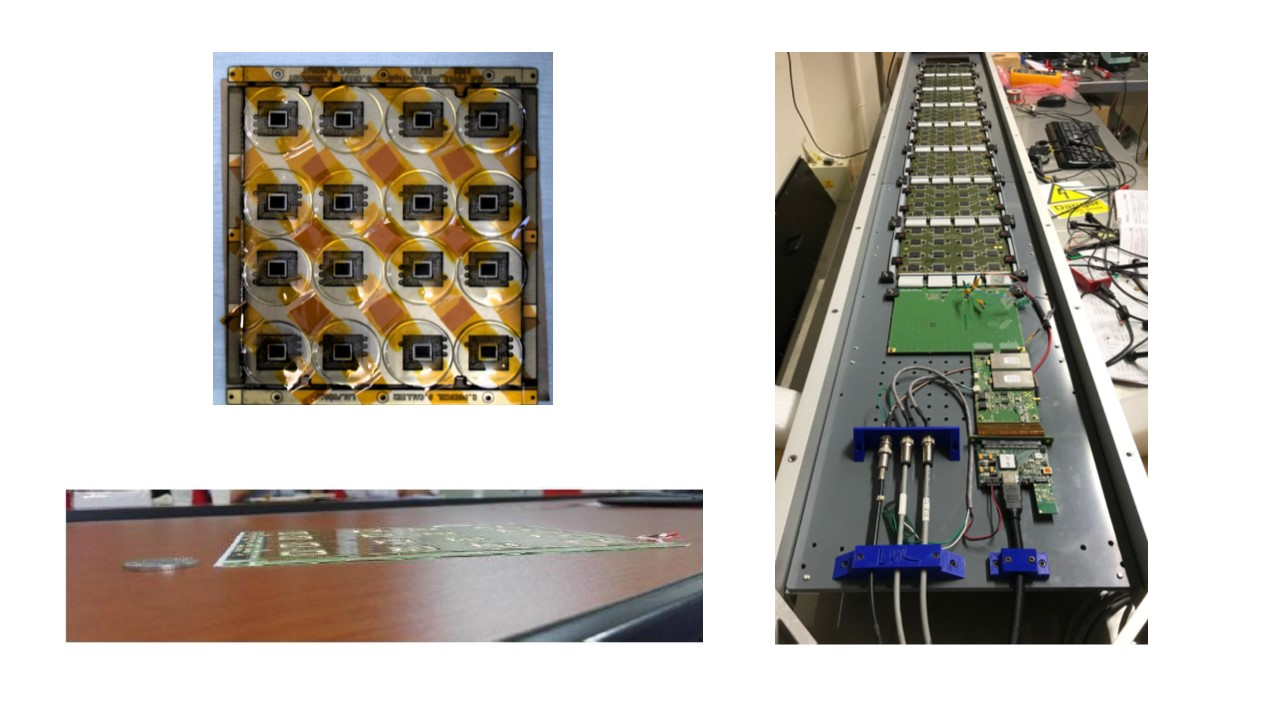
\includegraphics[width=1.0\hsize]{Detector/fig/SiWECAL_dev.jpg}
\caption{SiECAL developments towards the final detector: thin chip-on-board sensors (left) and long slabs corresponding to ILD dimensions (right).}
\label{fig:det:SiWECAL_dev}
\end{figure}

The Silicon technology developed for ILD has been retained as the baseline for the electromagnetic section of the CMS High Granularity Calorimeter (HGCAL) upgrade~\cite{Collaboration:2293646}. The HGCAL layout is based on hexagonal readout modules with a technology similar to the ILD one. It incorporates a new version of the SKIROC ASIC with a sub-ns timing functionality which may also be of interest for the ILD detector. A HGCAL prototype of 27 layers has been successfully tested by CMS in a combined beam test at CERN with the AHCAL ILD prototype (next section). The full HGCAL represents a 10\% prototype of the ILD SiECAL as regards the number of channels. Its construction will be a strong asset to validate the large scale assembly and fabrication processes for ILD. 

%\textit{Sc-ECAL results from new detector unit in construction.}

\subsubsection{Scintillator option (ScECAL)}

Similarly to the silicon option, the scintillator option of the electromagnetic calorimeter,
after the validation of the concept using the physics prototype,
has focused its R\&D towards a technological prototype 
with fully integrated detection layers. 
The design of the detection layer is based on an integrated readout board, 
called ECAL base unit (EBU), of $18\times18\,\mathrm{cm}^2$ 
with four SPIROC ASICs developed by OMEGA group\cite{ild:bib:spiroc} on which 144 scintillator strips 
($5\times45\times2\,\mathrm{mm^3}$ each) coupled to SiPMs are mounted.

Notable progresses have recently been made on the SiPMs for the ScECAL. 
MPPCs with a smaller pixel pitch of 10 or $15\,\mu\mathrm{m}$ have been developed 
by Hamamatsu Photonics K.K, which can provide a larger dynamic range required 
for the ScECAL\cite{ild:bib:hdmppc}. 
Further improvements have been made for the most recent small-pixel MPPCs, 
including reduced optical cross-talk by a trench structure between pixels, 
lower dark noise and higher PDE, which have been confirmed by the prototype tests.

In the previous prototype studies, the SiPM was attached to the side edge 
of the strip. 
New designs of the SiPM readout at the bottom side of the strip 
are being developed for more uniform response and a better compatibility 
with future large-scale production.
Especially a recently proposed design based on a strip 
with a dimple directly coupled to a surface-mounted SiPM on the PCB, 
which is similar to the SiPM-on-tile technology of AHCAL,
shows a promising performance.

Low cost and high light yield plastic scintillator materials are also being developed 
for the ScECAL.
The development focuses on the polystyrene-based scintillator 
produced by the injection moulding method, which is suitable 
for large-scale production. 
A reasonably high light yield of 65--70\% compared to that of 
the commercial PVT-based scintillator has been achieved 
by optimizing the production parameters. 

Detection layer prototypes have been developed 
with the small pixel MPPCs ($15\,\mu\mathrm{m}$ pixel pitch) 
as shown in the left of Figure~\ref{fig:det:ScWECAL_prototype}.
A prototype layer was tested in positron beams of 50--800\,MeV 
at ELPH of the Tohoku University.
The right of Figure~\ref{fig:det:ScWECAL_prototype} shows the typical charge distribution 
obtained for the positron beam where the MIP peak is well separated 
from the pedestal.

\begin{figure}[htb]
\centering
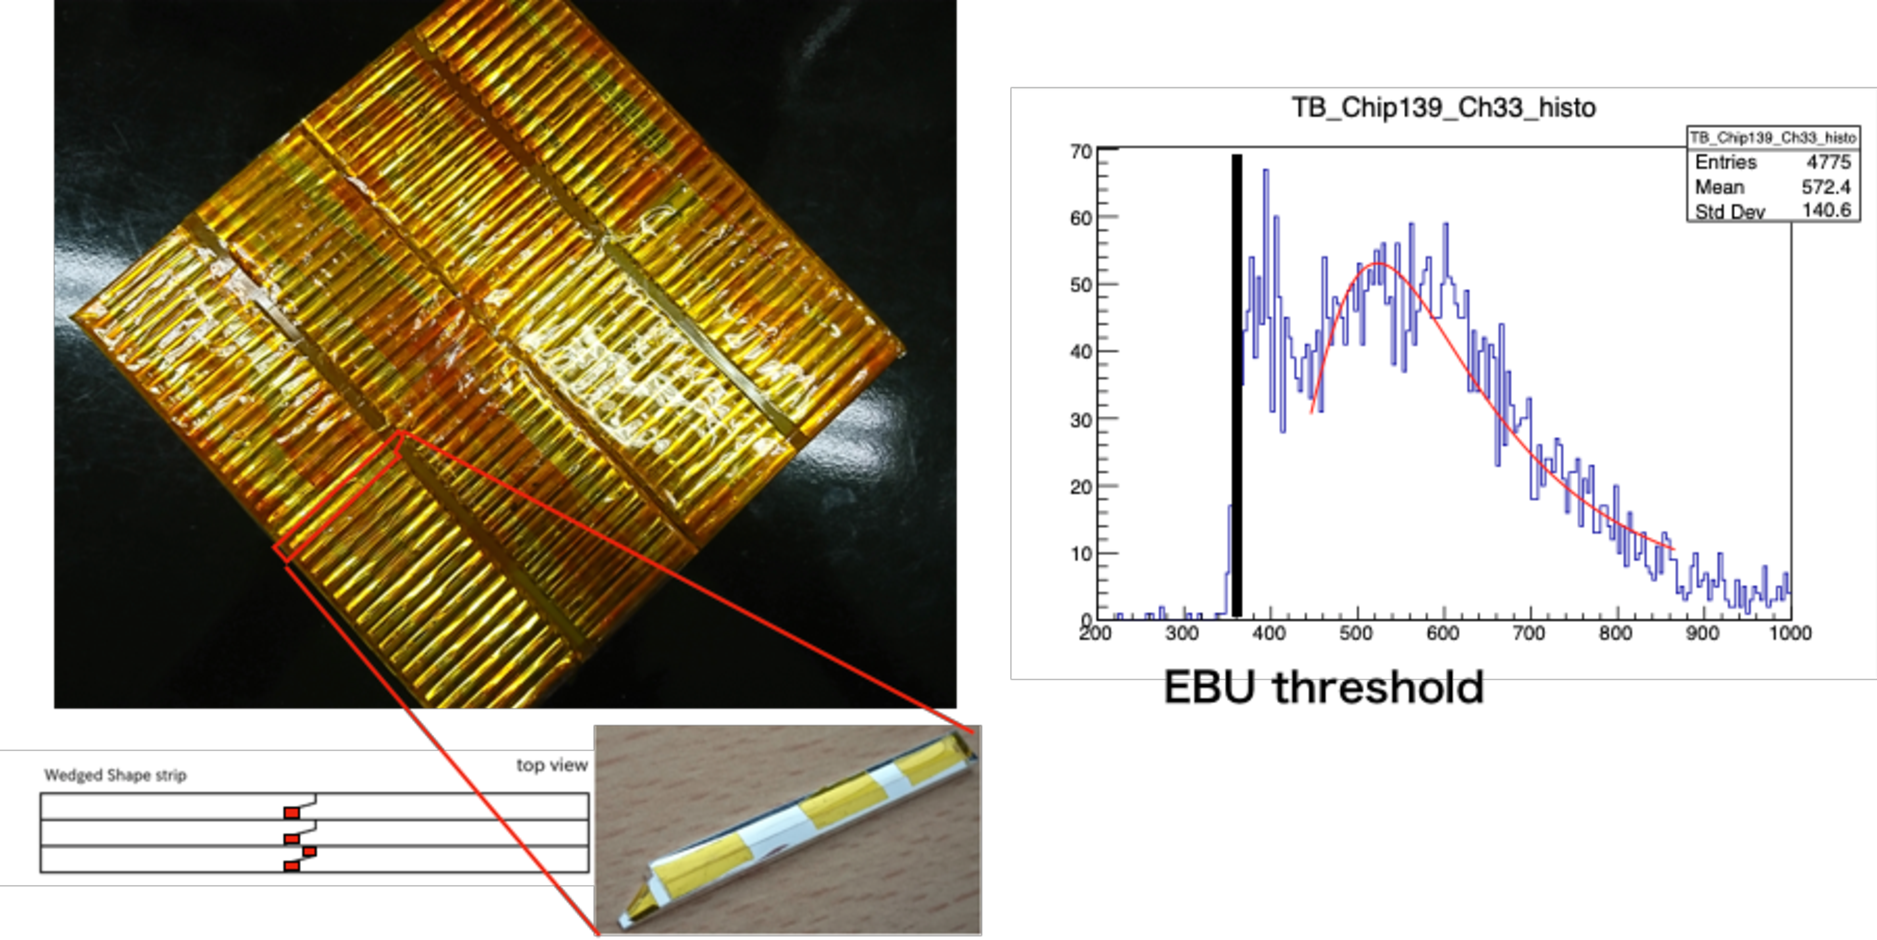
\includegraphics[width=1.0\hsize]{Detector/fig/ScWECAL_prototype.pdf}
\caption{(Left) Prototype detection layer with small pixel MPPCs  
   and (right) typical charge distribution obtained for positron beam 
where a MIP peak is well separated from the pedestal.}
\label{fig:det:ScWECAL_prototype}
\end{figure}


A fully integrated technological prototype with 30 alternating absorber and detection 
layers is planned to be constructed 
as a joint effort with the ScECAL R\&D for CEPC 
to demonstrate the performance of the ScECAL technology 
and its scalability to the full-size detector. 

\vspace{2cm}

\subsection{Hadronic Calorimeter}
\label{ild:sec:HCAL}
%\writer{Felix Sefkow, Imad Laktineh}{4}
%\textit{AHCAL beamtest results from large technological prototype, CMS HGCAL spinoff.}

\subsubsection{Scintillator option (AHCAL)}

A CALICE AHCAL physics prototype had been built and operated in 2006-2011, allowing to demonstrate the particle flow~\cite{Adloff:2011ha} and energy resolution performance~\cite{Adloff:2012gv} of the scintillator SiPM ("SiPM-on-Tile") technology for the DBD. In subsequently published papers~\cite{Adloff:2013vra,Adloff:2013kio,Adloff:2013jqa,Adloff:2014rya,Bilki:2014bga,Lucaci-Timoce:2013tkf,Price:2016sce} the adequate modelling of instrumental effects and shower evolution has been further established, and the hadronic energy resolution and linearity of a combined system with a scintillator tungsten ECAL in front was shown~\cite{Repond:2018flg} to be as good as that of the AHCAL alone, see Fig.\ref{fig:ahcal-linres}. The software used to model the detector effects such as photo-electron statistics in the SiPM has been validated by the test beam data and is also used in ILD, after adjusting for a small difference in sampling fraction only~\cite{Hartbrich:2016bbz}.
\begin{figure}[hbt]
\centering
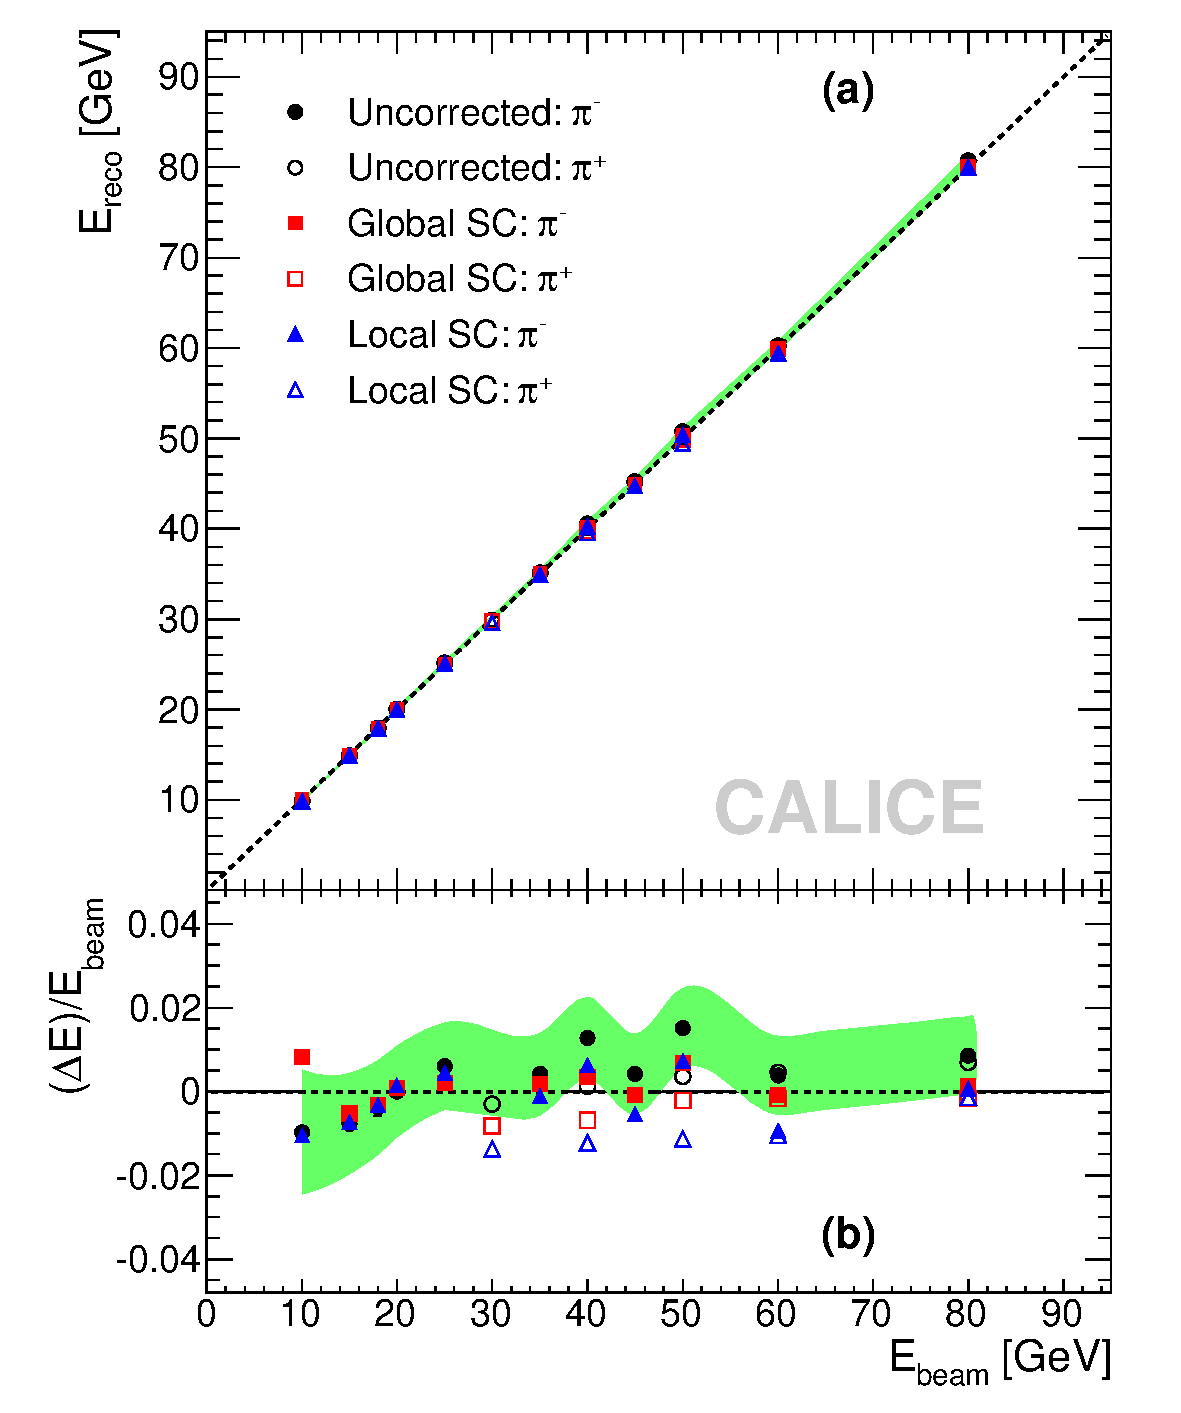
\includegraphics[width=0.39\textwidth]{Detector/fig/AHCAL-Linearity_Ini_GC_LC.pdf}
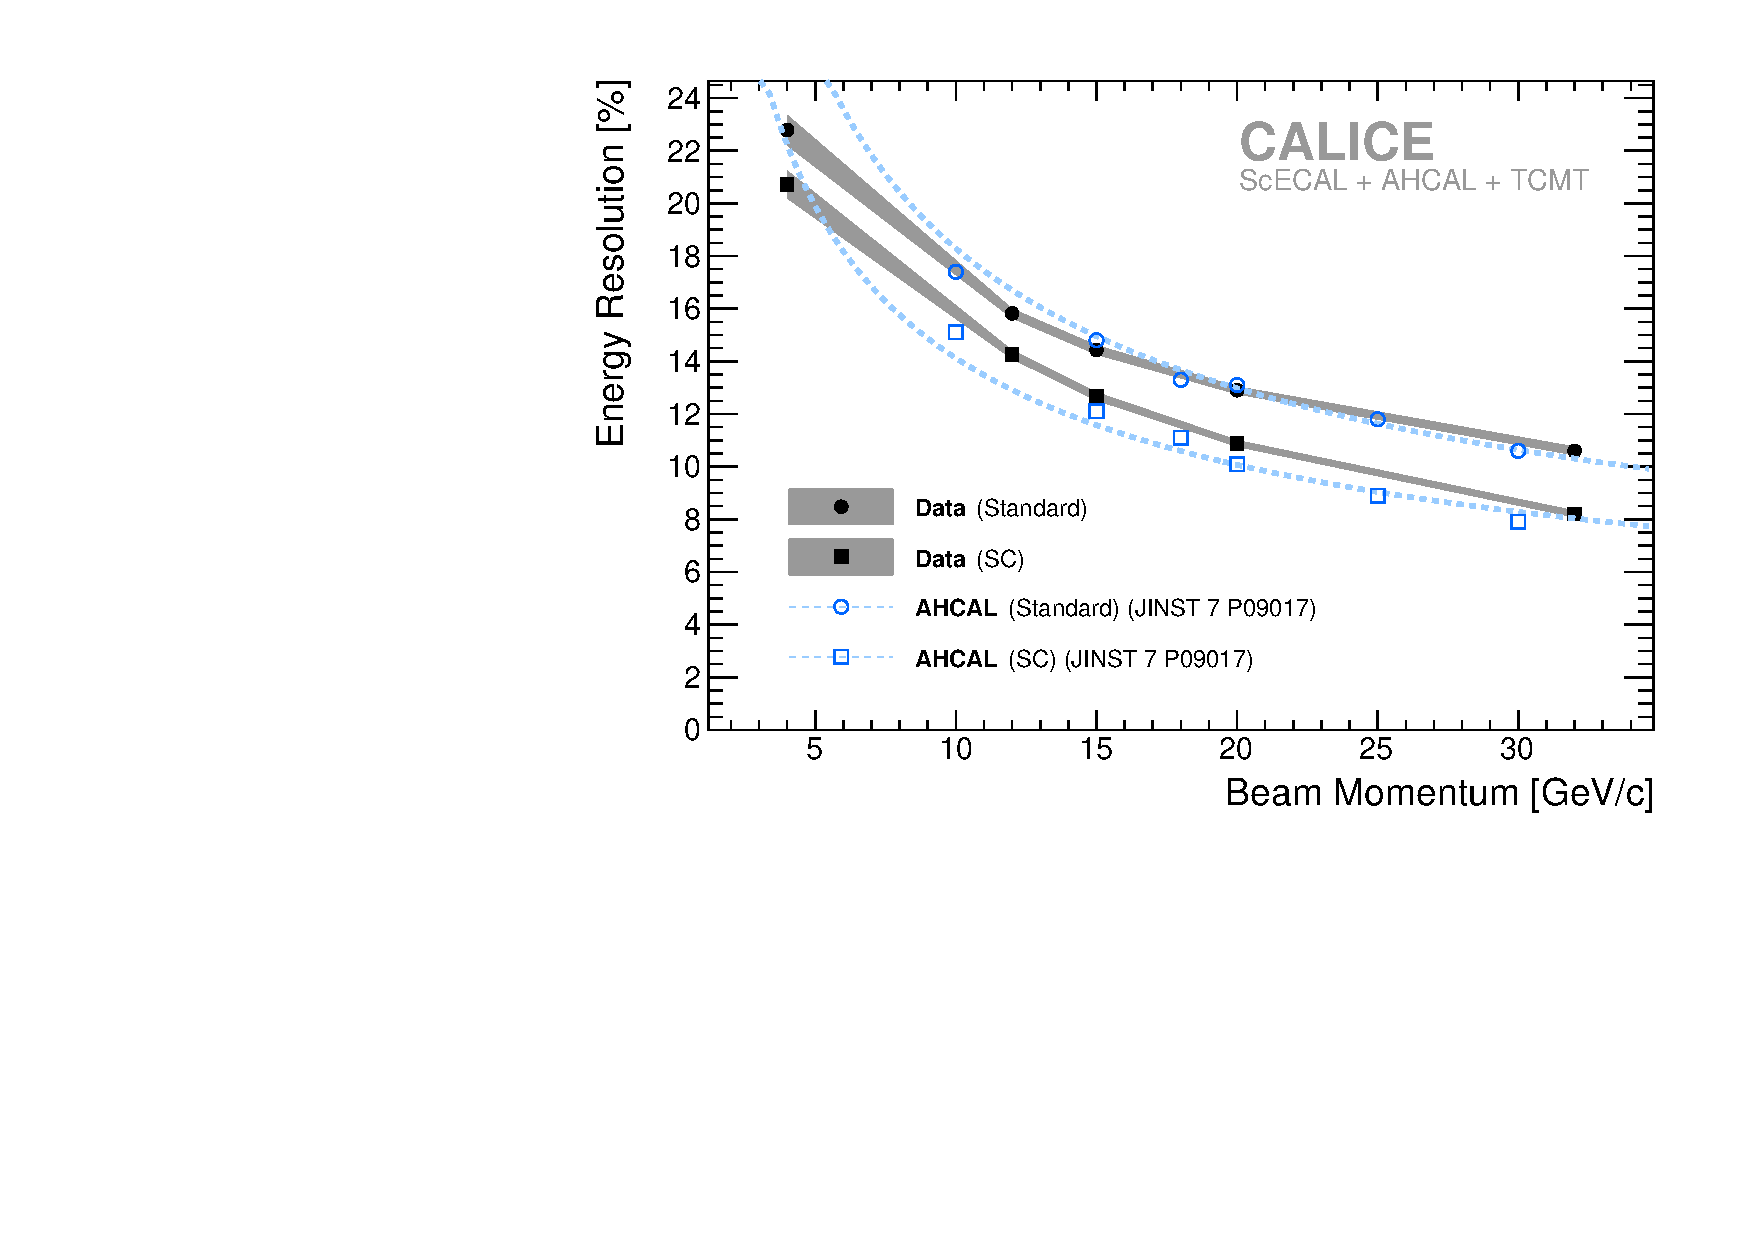
\includegraphics[width=0.59\textwidth]{Detector/fig/AHCALpion_resolution_data_ahcaljinst.pdf}
\caption{Performance of the CALICE AHCAL physics prototype for pions. Left: Response without and with global or local software compensation for the AHCAL alone (with tail-catcher, from~\cite{Adloff:2012gv}). Right: resolution of the AHCAL with ("Standard") and without ("SC") a scintillator ECAL in front (from~\cite{Repond:2018flg})}
\label{fig:ahcal-linres}
\end{figure}

With the establishment of the principal viability of the AHCAL technology, the focus has shifted from the study of the physical performance characteristics of such a detector to the demonstration of the feasibility of the concept while satisfying the spatial constraints and scalability requirements of collider experiments such as ILD. For this purpose a new AHCAL technological prototype has been built. It is based on a scintillator tile design well-suited for mass production and automatic assembly, originally proposed in~\cite{Blazey:2009zz} and subsequently varied and optimised in further studies \cite{Simon:2010hf, Liu:2015cpe}. 

The new AHCAL technological prototype~\cite{Sefkow:2018rhp} consists of a non-magnetic stainless steel absorber structure with 38 active layers and has 21888 channels. 
The structure has been produced from standard rolled plates, which had undergone a cost-effective roller-levelling procedure, ensuring a flatness of $\pm 1$~mm, demonstrated over an area of 2$\times$2~m$^2$. The plates were assembled using screws as foreseen for the full ILD structure in the TESLA mechanical layout. 
The basic unit of the active elements is the HCAL Base Unit HBU~\cite{Reinecke:2013zua}, with a size of 36 $\times$ 36 cm$^2$, holding 144 SiPMs controlled by four SPIROC2E ASICs \cite{Bouchel:2011zz}.  A key element of the electronics is the capability for power-pulsed operation.
%to reduce the power consumption and eliminate the need for active cooling, making use of the low duty cycle in the linear collider beam time structure. 
In addition to dual-gain energy measurement, the electronics also provides a cell-by-cell auto trigger and time stamping on the few ns level in test beam operations. In operating conditions with shorter data-taking windows closer to the bunch train structure of linear colliders, sub-ns time resolution is achieved. 

The prototype uses Hamamatsu MPPC S13360-1325PE photon sensors and injection-moulded polystyrene scintillator tiles with a central dimple \cite{Liu:2015cpe} for optimal light collection, as shown in Fig.~\ref{fig:AHCAL-TileProto}. 
\begin{figure}[hbt]
\centering
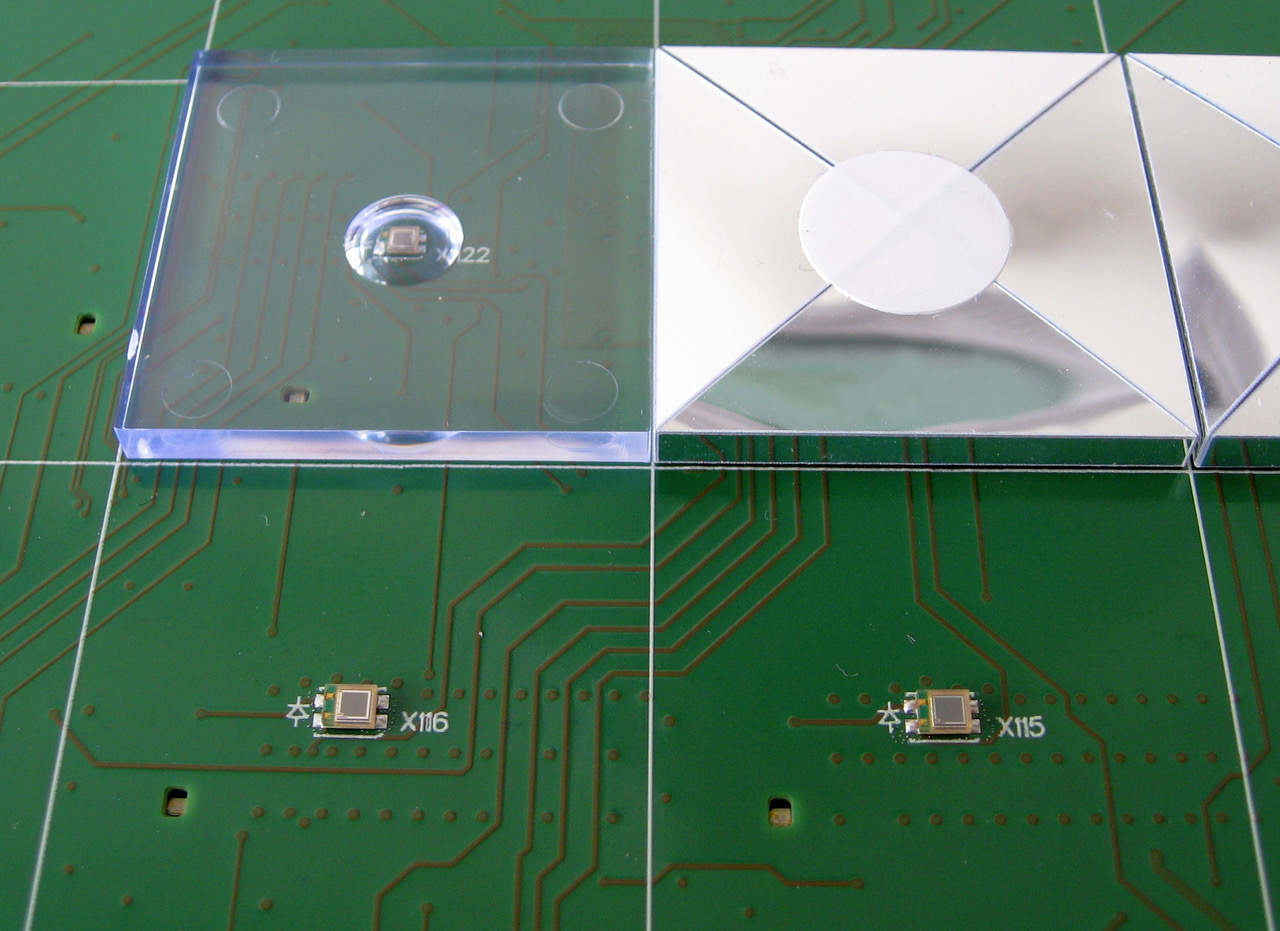
\includegraphics[width=0.39\textwidth]{Detector/fig/hcal-tiles.jpeg}
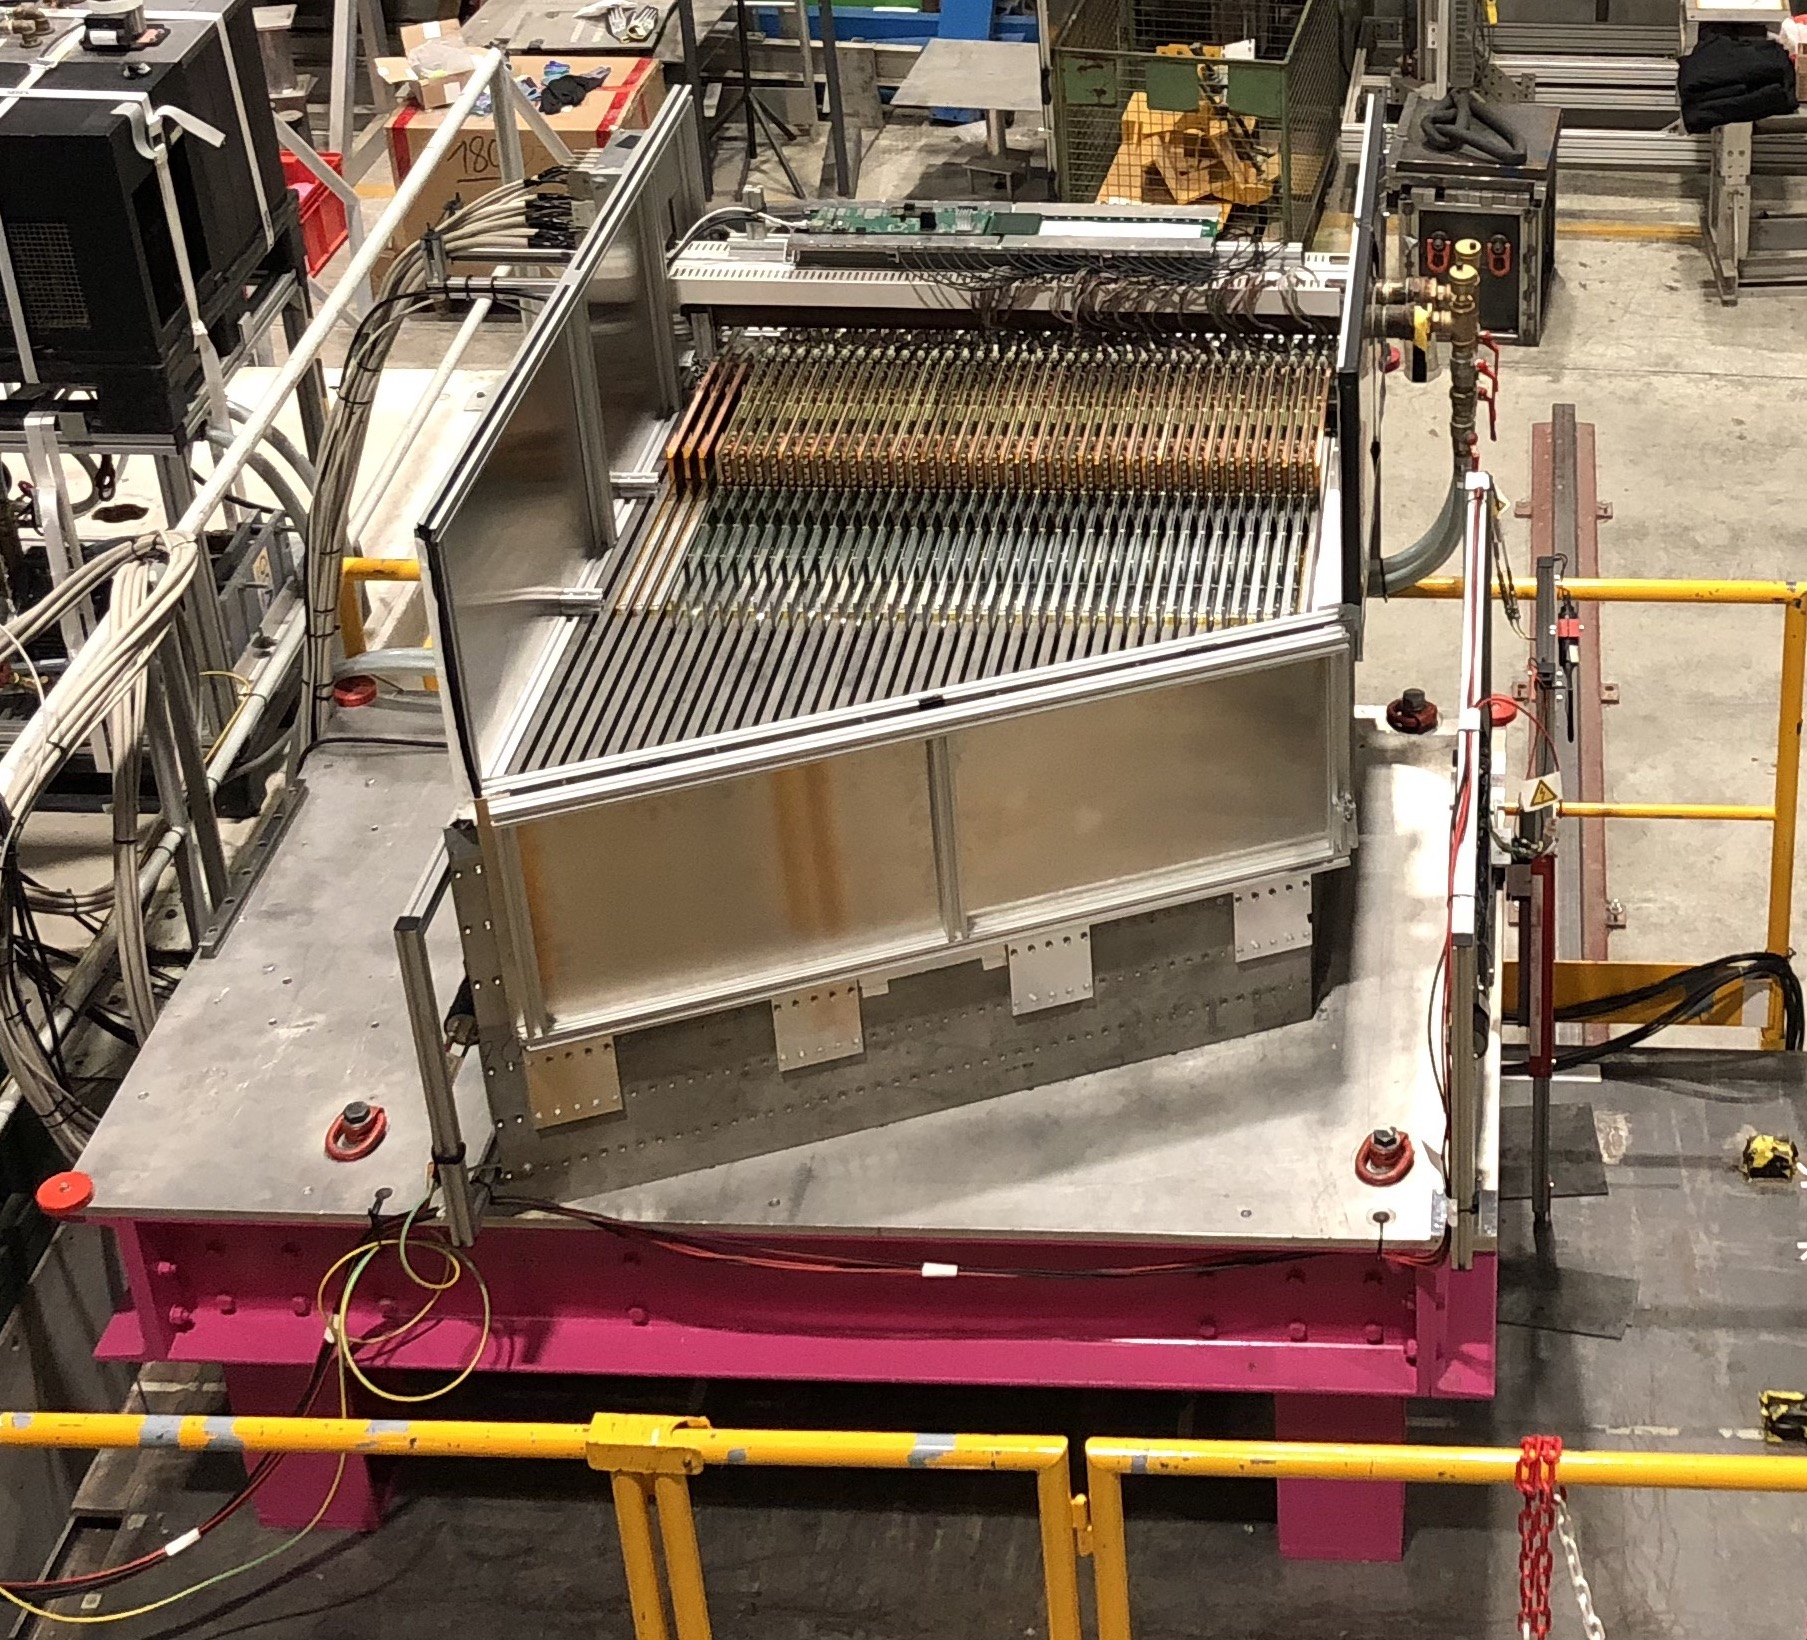
\includegraphics[width=0.59\textwidth]{Detector/fig/AHCAL-prototype.jpeg}
\caption{The AHCAL technological prototype. Left: Read-out board (HBU) with SiPMs and (un-)wrapped tiles. Right: Prototype installed in the H2 beam line at the CERN SPS.} 
\label{fig:AHCAL-TileProto}
\end{figure}
%
%The SiPMs were delivered in lots of 600 pieces with a uniform break-down voltage within $\pm 100$~mV. 
Spot-samples of all SiPM lots, and each one of the ASICs, had undergone semi-automatic testing procedures before soldering the HBUs \cite{Munwes:2634923}. The gain of the SiPMs was found to be uniform within~2.4\% when operated at a common over-voltage.
Without any further surface treatment, the scintillator tiles are wrapped in laser-cut reflective foil by a robotic procedure and mounted on the HBUs using a pick-and-place machine, after glue dispensing with a screen printer.   
%
The HBUs have been integrated into cassettes with interfaces for DAQ \cite{Kvasnicka:2017bpx}, LED pulsing and power distribution, which provide active compensation of temperature variations by automatic adjustments of the common bias voltage of the photon sensors in each layer. This was routinely used in test beam operation and stabilises the gain within $\pm 1\%$.
%Figure~\ref{fig:ActiveLayer} shows the top side of one active layer, with the scintillator tiles visible. 
%All layers have been  calibrated in the DESY test beam, and 99.96\% of the total 21888 channels are working.
%\begin{figure}
%\centering
%\includegraphics[width=0.7\textwidth]{figures/Layer-backside.jpg}
%\caption{Active layer side with wrapped tiles on 4 HBUs, with %\label{fig:ActiveLayer}
%\end{figure}
%
%The active layers were calibrated in the DESY test beam, assembled into the absorber stack and connected to 
Data concentration, power distribution and cooling service systems of the prototype are also scalable to the full ILD detector. 
%Figure~\ref{fig:AbsorberStructure} shows the active layers with connected services inserted in the absorber structure.
%\begin{figure}
%\centering
%\includegraphics[width=0.7\textwidth]{figures/AHCAL2.jpg}
%\caption{SiPM-on-tile AHCAL engineering prototype.}
%\label{fig:AbsorberStructure}
%\end{figure}

%The full prototype 
%has been commissioned with cosmic muons, exploiting its self-triggering capabilities and then
%; see Figure~\ref{fig:EventDisplay}.
%Two event displays are shown from cosmic rays interacting in the calorimeter. The top figures is a straight track from a minimum-ionising muon and the bottom is most likely a shower developed from an inelastic interaction of a muon with the absorber material.
The AHCAL technological prototype was installed in the test beam for data taking at the CERN SPS, see Fig.~\ref{fig:AHCAL-TileProto}.
During two periods in May and in June 2018, several $10^7$ events with muon tracks, as well as electron and pion showers in the energy ranges  10 -- 100~GeV and 10 -- 200~GeV, respectively, have been recorded. 
%The data taking rate averaged over the about 5~s long spills was up to 400 events per second.
Figure~\ref{fig:AHCAL-nhit-longslab} from the quasi-instantaneous data quality monitoring shows the distribution of the number of hits vs.\ the hit-energy weighted centre-of-gravity (cog) along the beam axis z for an electron run with a beam momentum of 100~GeV/c and admixtures of muons and hadrons. The different particle types populate different regions of the plot.
\begin{figure}[hbt]
\centering
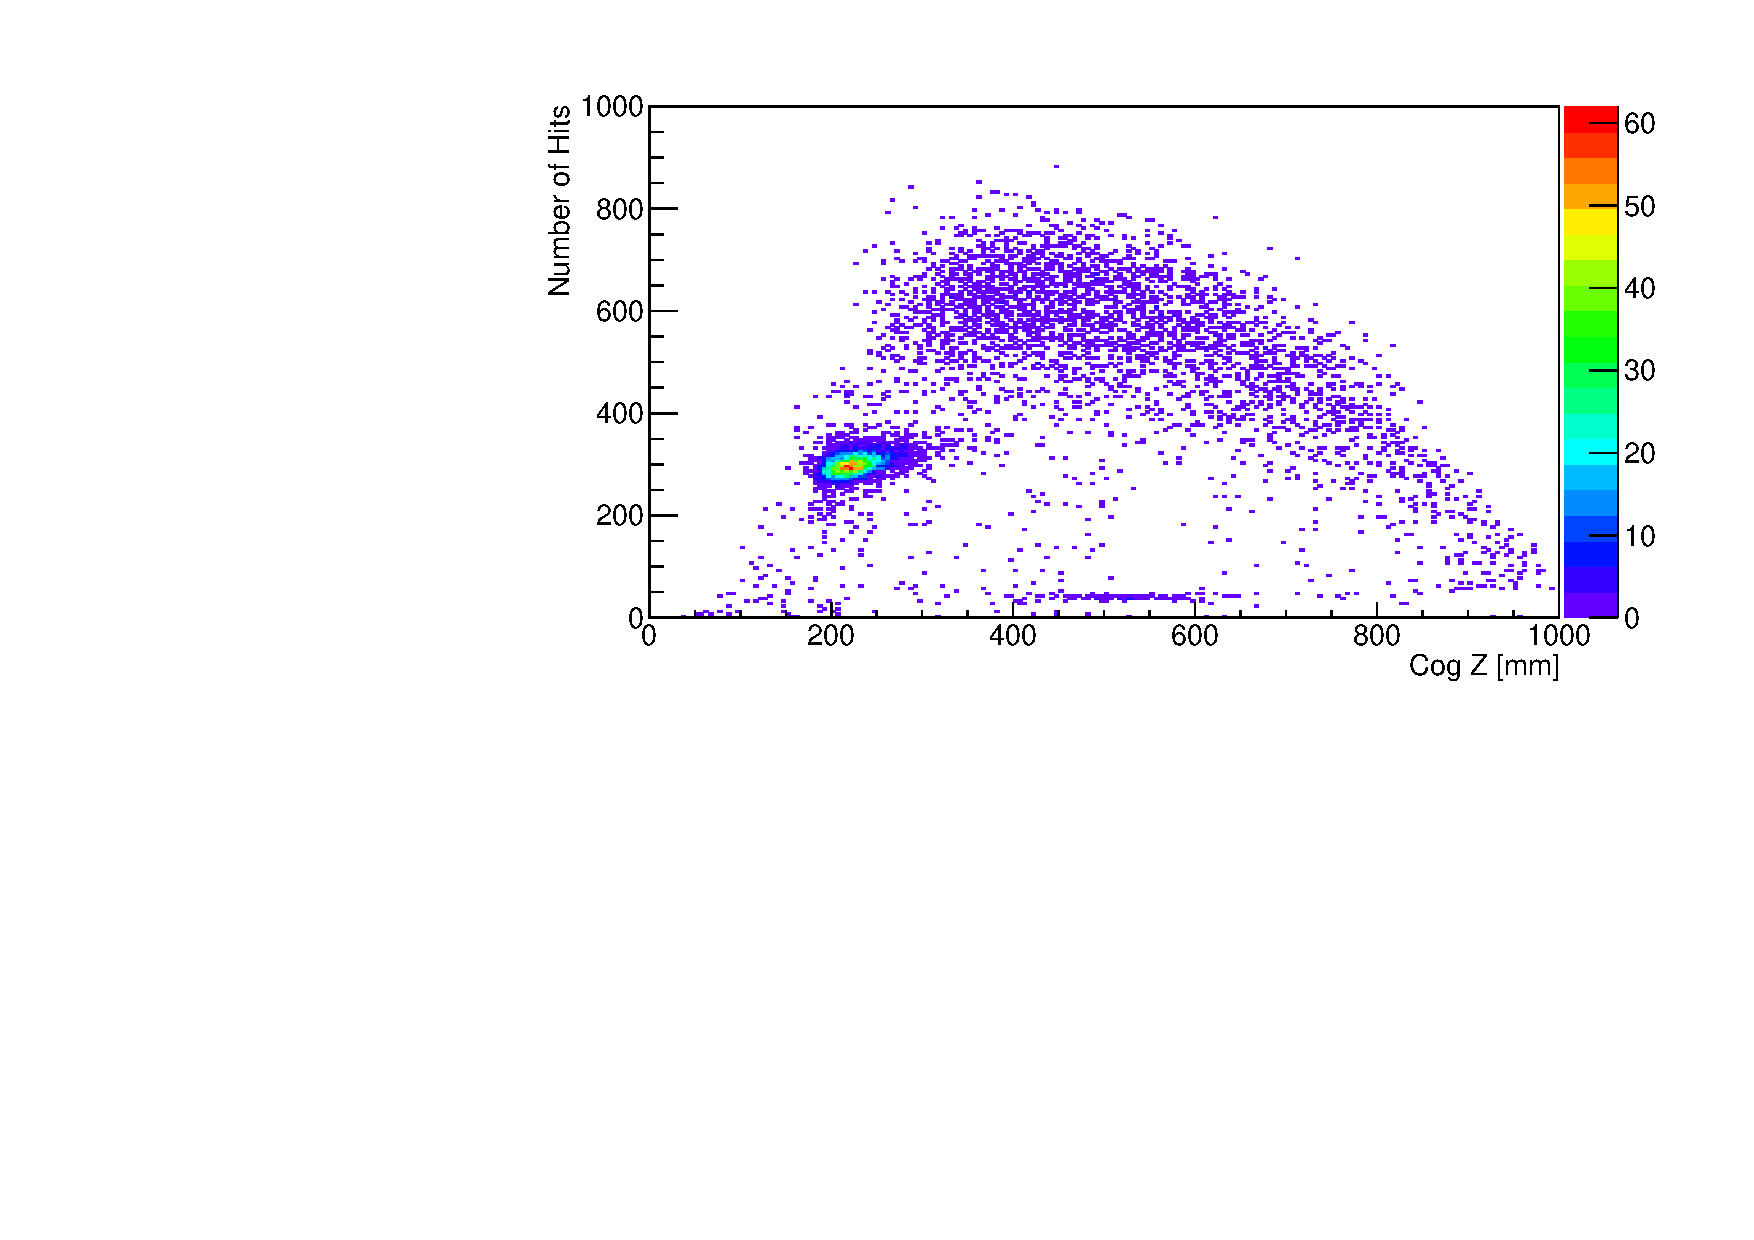
\includegraphics[width=0.64\textwidth]{Detector/fig/AHCAL-cogz_nhits.pdf}
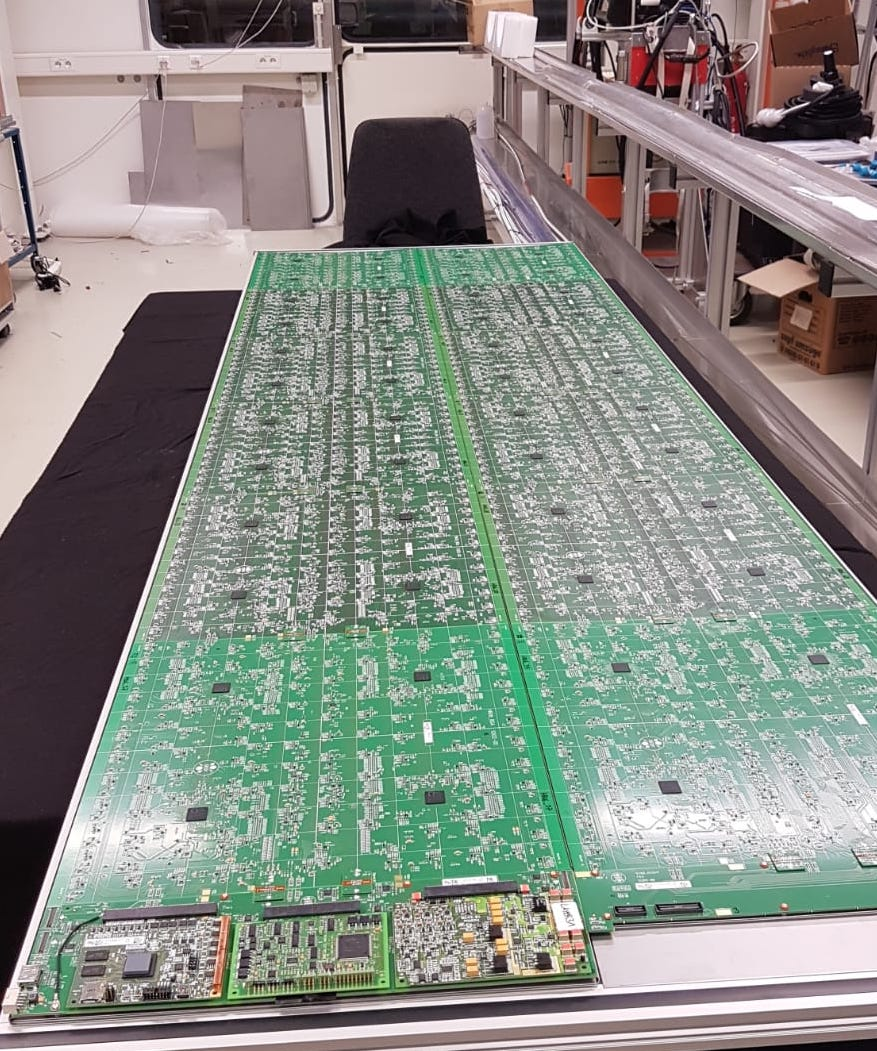
\includegraphics[width=0.34\textwidth]{Detector/fig/AHCAL-LomgSlab.jpeg}
\caption{Left: Distribution of the number of hits vs.\ the hit-energy weighted centre-of-gravity (cog) for a mixed beam in the AHCAL technological prototype. Right: Two slabs of HBUs with interfaces, corresponding to full ILD length in the TESLA configuration.} 
\label{fig:AHCAL-nhit-longslab}
\end{figure}
%
While electron showers are characterised by a relatively narrow distribution of number of hits and a cog near the front face of the detector, hadrons exhibit a wider distribution of the cog, and a larger number of hits, decreasing as the cog moves towards the rear of the detector, and leakage increases.
Muons appear as a narrow band with $\sim 38$ hits and a cog on z ay about half the depth of the detector. 

%The figure shows how the detailed topological information of the AHCAL can be used for the identification of particle types. The width of the distribution for electrons, and tails towards lower number of hits, suggest a compromised beam quality for the May period shown here, which indeed was resolved for the June period.
%
%\section{Conclusions}
%A highly granular hadron calorimeter prototype with 21888 channels, based on 3$\times$3~cm$^2$ scintillator tiles and SiPMs integrated with the embedded read-out electronics, has been successfully constructed and operated in test beams. The scalable design and automated construction and quality assurance procedures validate the concept for linear collider detector applications. 
%
The rich data sample collected in the two test beam periods in 2018  is being used for shower separation studies based on 5-dimensional reconstruction algorithms exploiting the high spatial, energy and time resolution of the prototype. 
While this is in progress, it can already be noted that in several aspects the  performance exceeds that of the physics prototype: the noise is a factor 100 lower, the dynamic range of the SiPMs is 3 times larger, and 99.96\% of the total 21888 channels are working.

The HBUs of the new prototype have also been used to build a large layer with two slabs of 6 HBUs each, corresponding to the full length of an ILD barrel sector in the TESLA layout, see Figure~\ref{fig:AHCAL-nhit-longslab}. The signal quality was unaffected, and the rise time of the power pulsing was within specifications. 

The AHCAL developments have also inspired the design of the scintillator section of the CMS end-cap calorimeter upgrade for the high luminosity phase of the LHC~\cite{Collaboration:2293646}, and the new prototype has been used together with silicon-instrumented sections in front in a common beam test, further illustrating the maturity of the technology. 
The new CMS endcap calorimeter will establish the SiPM-on-Tile technology in a collider environment at an intermediate scale between the AHCAL prototype and the full ILD detector. 

\subsubsection{RPC option (SDHCAL)}

The SDHCAL technological prototype built in 2011 has been regularly tested in beams in the past years with various configurations, including a combined test with the SiECAL prototype in 2018 (previous section). The SDHCAL prototype consists in 48 single-gap RPC layers of 1 $m^2$ (Figure~\ref{fig:det:SDHCAL_proto}). Each detection gap is instrumented with 6 Active Sensitive Units (ASU) made of a  50 x 33 $cm^2$ PCB with 24 "HARDROC" ASICs from OMEGA~\cite{Callier:2014uqa}. The RPC pad size is 1 $cm^2$ and the pad signals can be readout either in digital (1 bit and 1 threshold) or semi-digital (2 bits and 3 thresholds) modes.

\begin{figure}[t!]
\centering
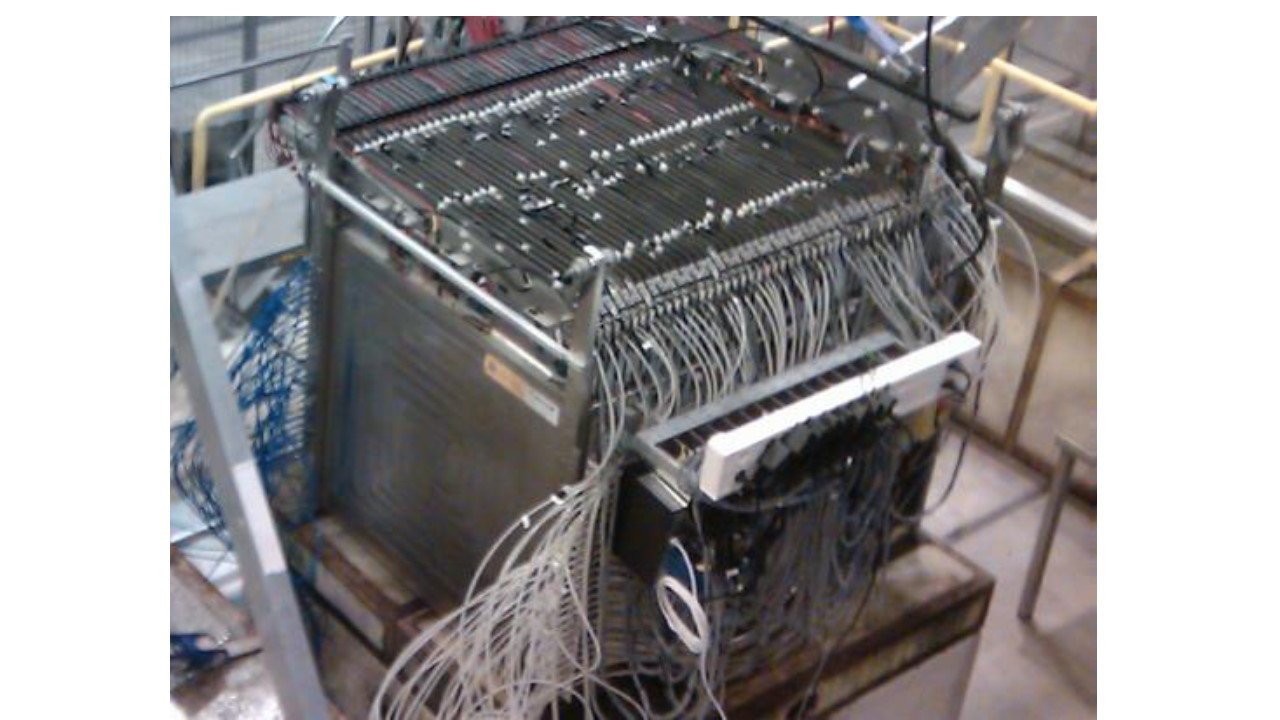
\includegraphics[width=0.8\hsize]{Detector/fig/SDHCAL_proto.jpg}
\caption{Technological prototype of the Semi-Digital Hadronic Calorimeter.}
\label{fig:det:SDHCAL_proto}
\end{figure}

The numerous data sets collected at CERN with high-energy hadron beams have been used to validate the performance of the technology. Special reconstruction methods adapted to the high granularity semi-digital structure of the calorimeter have been developed~\cite{Buridon:2016ill} to relate the energy estimation to the hit number and density. The current state of the performance is summarized in Figure~\ref{fig:det:SDHCAL_perf}. A good linearity is observed and the multi-threshold mode is found to mitigate saturation and improve the resolution at high energy. The description of the measured resolution by the simulation is however found to be sensitive to the description of the core of the hadronic showers, with a tendency for the Monte-Carlo to underestimate the performance due to harder cores in the showers~\cite{Deng:2016obt}. This point will require further tuning of the simulation.

\begin{figure}[t!]
\centering
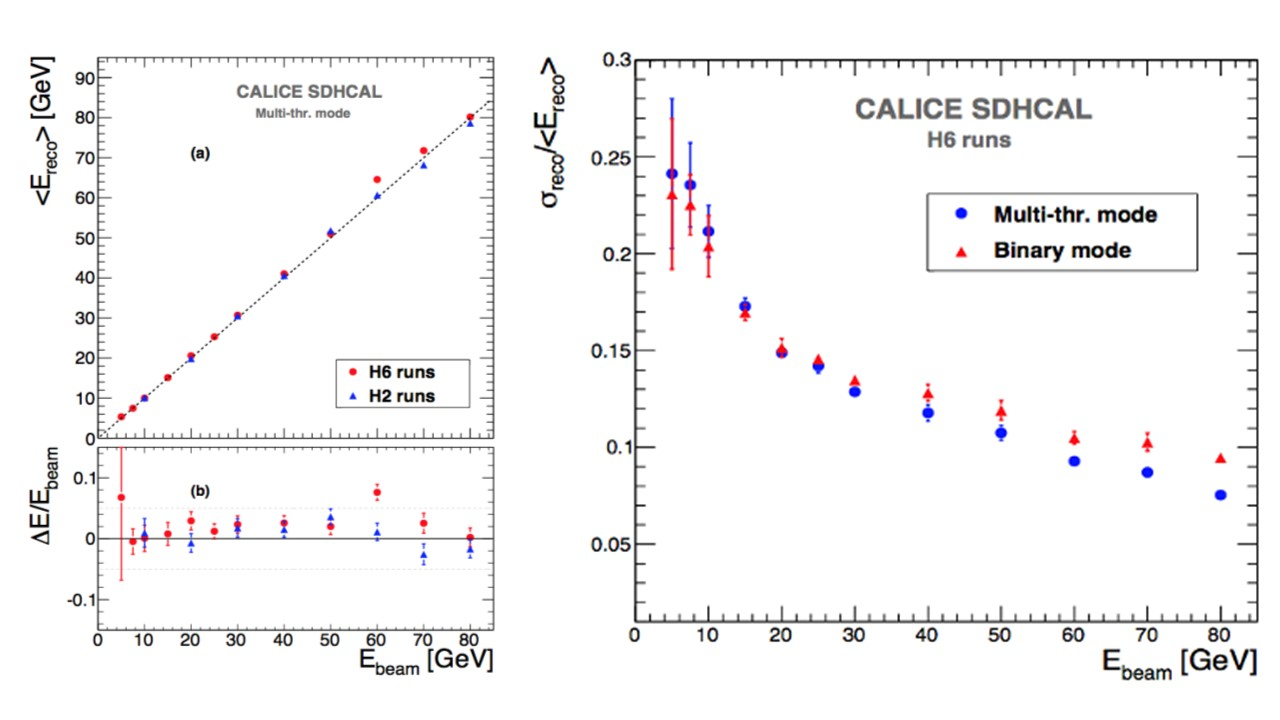
\includegraphics[width=1.0\hsize]{Detector/fig/SDHCAL_performance.jpg}
\caption{Performance of the SDHCAL technological prototype as measured in beam tests: linearity (left) and energy resolution for the digital and semi-digital readout options (right).}
\label{fig:det:SDHCAL_perf}
\end{figure}

In the recent years the SDHCAL teams have focused on adapting the technology to the full-size ILD requirements, in order to cover detection surfaces of up to 1 x 3 $m^2$ required by the ILD Hadronic Calorimeter in its "Videau" configuration (section 5.1.2). An improved RPC gas circulation system with better uniformity has been designed and validated with the construction of two large RPC's. Larger ASUs of 100 x 33 $cm^2$ have been designed with a new version of the HARDROC ASIC including 0-suppression (Figure~\ref{fig:det:SDHCAL_dev} left), and their interconnection improved to allow chaining of up to 9 ASUs. Efforts have also been invested in the manufacturing process of self-sustained hadron calorimeter structures with high precision mechanical tolerance as required by the RPC insertion. A method of "roller levelling" has been used to machine steel absorber plates with a high flatness. A high precision electro-welding has been used to built a first large size prototype of 4 calorimeter layers (Figure~\ref{fig:det:SDHCAL_dev} right) which has proven that gap size variations well below 1 mm can be reached on such large structures. 

For the longer term the option of multi-gap RPC's with a high timing resolution of $\approx$20 ps is prototyped based on the "PETIROC" ASIC~\cite{Fleury:2014hfa}. 

\begin{figure}[t!]
\centering
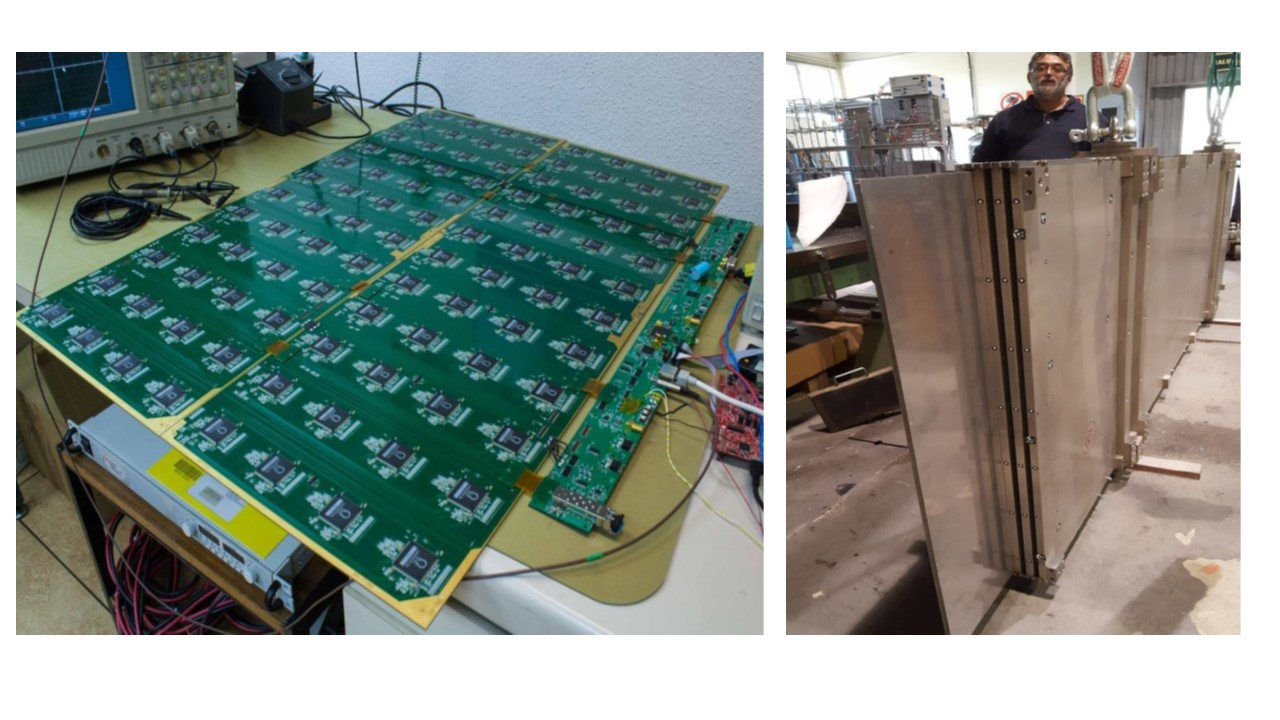
\includegraphics[width=1.0\hsize]{Detector/fig/SDHCAL_dev.jpg}
\caption{SDHCAL ongoing developments for the final ILD dimensions: two active sensor units of 100 x 33 $cm^2$ chained to each other and connected to the outside with a new compact DAQ interface (left), and self-sustained welded structure of 4 calorimeter plates of 1x3 $m^2$   with the required mechanical tolerances (right).}
\label{fig:det:SDHCAL_dev}
\end{figure}

\vspace{2cm}
\subsection{Very forward detectors}
\writer{Yan Benhammou, Sergej Schuwalow}{2}

In the past years the development of the ILD forward detectors has mostly been pursued by the FCAL R\&D Collaboration [ref]. Progress concerns mainly the LUMICAL calorimeter and, more recently, the BEAMCAL sensors.

Based on a specific ASIC [ref] developed after the DBD, calorimeter silicon sensitive layers have been built to assemble a first LUMICAL 4-layer tungsten calorimeter prototype and, two years later, a more compact 8-layer calorimeter prototype (Figure~\ref{fig:det:LUMICAL_perf} left). The two prototypes were beam-tested in 2014 and 2016, respectively. The test data [ref] confirm the expected significant improvement of the transverse compactness of the electromagnetic showers in the compact prototype compared to the earlier one (Figure~\ref{fig:det:LUMICAL_perf} right). 

A new ASIC "FLAME" [ref] based on 130 nm CMOS technology is currently under final validation. FLAME features the low power, in-situ digitisation and fast readout required by the final detector. A new $\approx$20- layers SiW calorimeter prototype based on FLAME, with specifications and configuration close to the final LUMICAL detector, is under construction and planned to be beam-tested in 2019. 

\begin{figure}[t!]
\centering
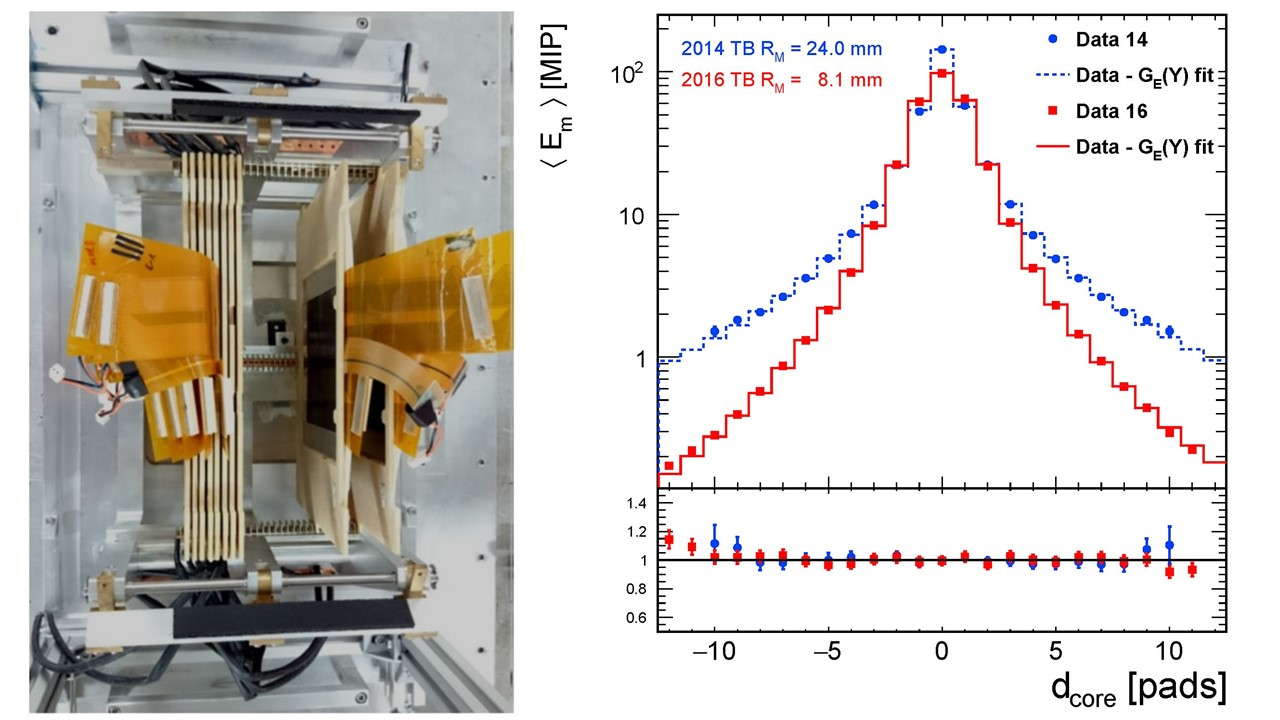
\includegraphics[width=1.0\hsize]{Detector/fig/LUMICAL_perf.jpg}
\caption{LUMICAL compact prototype tested in the DESY electron beam in 2016 (left) and corresponding improvement in shower compactness achieved versus the 2014 prototype (right).}
\label{fig:det:LUMICAL_perf}
\end{figure}

The LHCAL and BEAMCAL calorimeters can be based on similar technologies as the LUMICAL, with radiation hardness requirements increasing as function of the sensor proximity to the beam. For the BEAMCAL, new sensors such as sapphire are being considered. Irradiation campaigns are under way to characterize them (Figure~\ref{fig:det:LUMICAL_perf} right) and provide input for the final choice. 

\begin{figure}[t!]
\centering
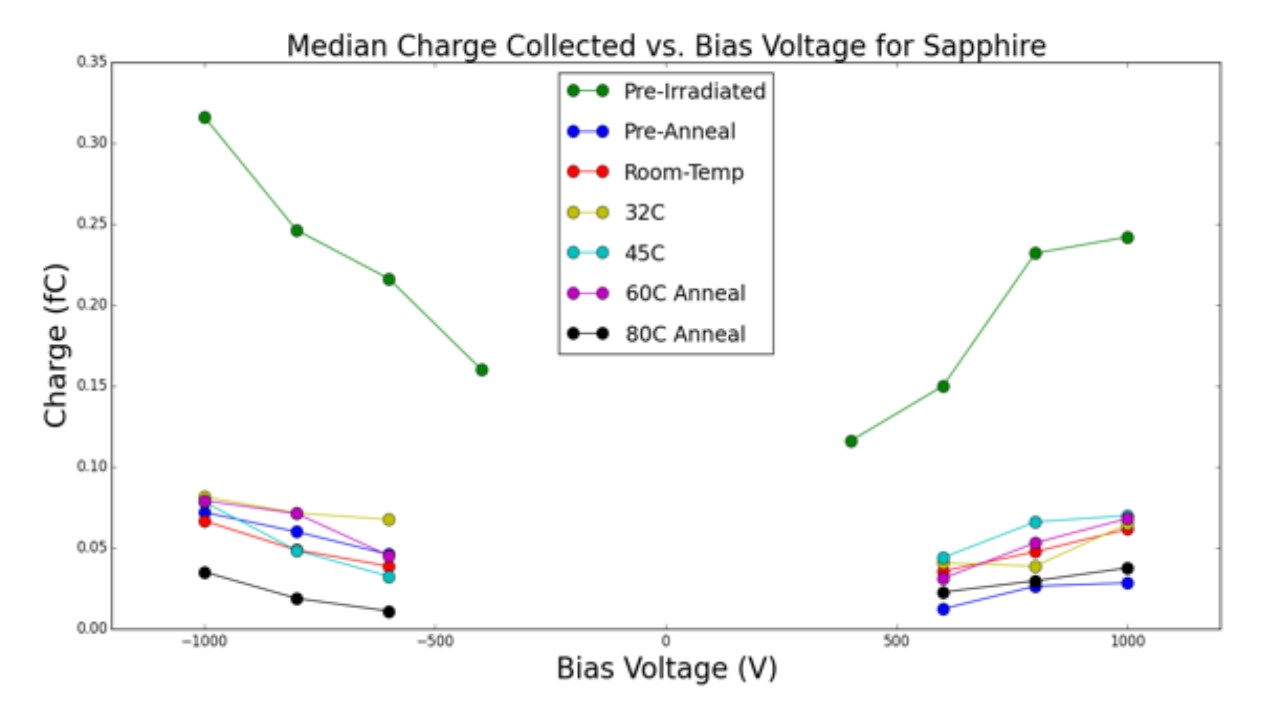
\includegraphics[width=0.8\hsize]{Detector/fig/BEAMCAL_rad.jpg}
\caption{results of irradiation tests performed at SLAC for sapphire sensors considered for the BEAMCAL.}
\label{fig:det:BEAMCAL_rad}
\end{figure}

\vspace{2.0cm}



\subsection{Iron instrumentation}
%\writer{Valery Saveliev}{1}

Dedicated studies have been conducted at FNAL in the past years to optimize the layout of scintillator bars adapted to muon detection. Prototypes have been built and tested with muon beams~\cite{Denisov:2015jjl}. They are all based on long scintillator bars with signal collected by WLS fibers and readout by SiPMs at both extremities. The transverse resolution of $\approx$1cm required for the muon momentum measurement is defined by the bar widths of a few cm. The longitudinal position is measured from the time difference of the signals of both extremities and depends on the WLS configuration. The two options under consideration described in section 5.1.2 (Figure~\ref{fig:det:yoke}) have been tested: longitudinal resolutions of 5 to 10 cm are measured and found roughly independent of the longitudinal position of the muon within the bar (Figure~\ref{fig:det:Iron_proto}). 

More studies are ongoing to develop low cost SiPMs also adapted to the measurement of the tails of high energy jets (tail catcher function). 

The RPC option for the iron yoke instrumentation was not specifically studied but would directly benefit from the RPC developments of the SDHCAL hadronic calorimetry option (section 5.2.4).   


\begin{figure}[t!]
\centering
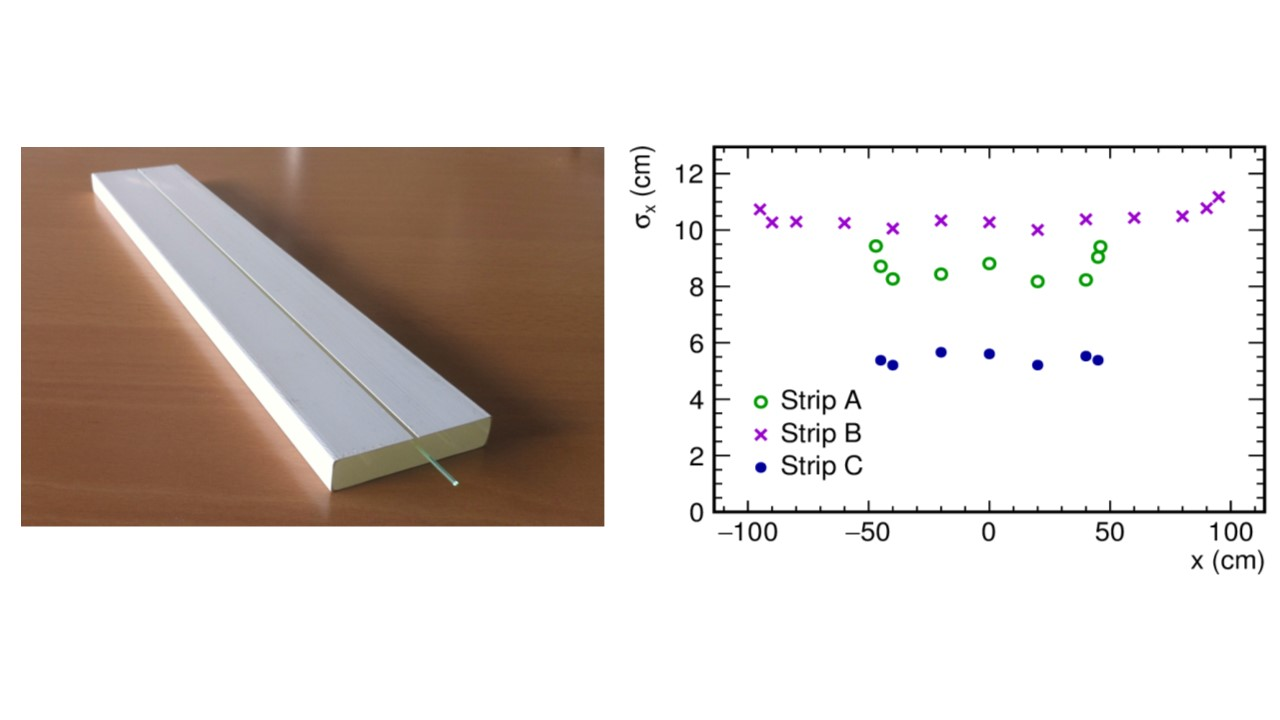
\includegraphics[width=1.0\hsize]{Detector/fig/Iron_proto.jpg}
\caption{Left: example of prototype scintillator bar built for the muon detector; right: longitudinal resolution on reconstructed muon as function of longitudinal coordinate: strip A and B as on left figure with lengths of 1 and 2 m respectively, strip C of 1m length with WLS fibers positioned on the small edge of the strip.}
\label{fig:det:Iron_proto}
\end{figure}

\vspace{2cm}
